\textbf{BUFR TABLES RELATIVE TO SECTION 3}

\textbf{BUFR/CREX Table B} \emph{-- Classification of elements}

F X Class Comments

0 00 BUFR/CREX table entries

0 01 Identification Identifies origin and type of data

0 02 Instrumentation Defines instrument types used

0 03 Instrumentation Defines instrument types used

0 04 Location (time) Defines time and time derivatives

0 05 Location (horizontal -- 1) Defines geographical position, including horizontal\\
derivatives, in association with Class 06 (first dimension of\\
horizontal space)

0 06 Location (horizontal -- 2) Defines geographical position, including horizontal\\
derivatives, in association with Class 05 (second\\
dimension of horizontal space)

0 07 Location (vertical) Defines height, altitude, pressure level, including vertical\\
derivatives of position

0 08 Significance qualifiers Defines special character of data

0 09 Reserved

0 10 Non-coordinate location (vertical) Height, altitude, pressure and derivatives observed or\\
measured, \emph{not} defined as a vertical location

0 11 Wind and turbulence Wind speed, direction, etc.

0 12 Temperature

0 13 Hydrographic and hydrological Humidity, rainfall, snowfall, etc.\\
elements

0 14 Radiation and radiance

0 15 Physical/chemical constituents

0 19 Synoptic features

0 20 Observed phenomena Defines present/past weather, special phenomena, etc.

0 21 Radar data

0 22 Oceanographic elements

0 23 Dispersal and transport

0 24 Radiological elements

0 25 Processing information

0 26 Non-coordinate location (time) Defines time and time derivatives that are not coordinates

0 27 Non-coordinate location Defines geographical positions, in conjunction with Class 28,\\
(horizontal -- 1) that are not coordinates

0 28 Non-coordinate location Defines geographical positions, in conjunction with Class 27,\\
(horizontal -- 2) that are not coordinates

0 29 Map data

0 30 Image

0 31* Data description operator Elements used in conjunction with data description\\
qualifiers operators

0 33 Quality information

0 35 Data monitoring information

0 40 Satellite data

0 41 \textbf{Oceanographic/biogeochemical parameters}

0 42 \textbf{Oceanographic elements}

\_\_\_\_\_\_\_\_\_\_\_\_

* This class does not exist in CREX.

\emph{(continued)}

\emph{\\
(BUFR/CREX Table B -- continued)}

Notes:

(1) Where a code table or flag table is appropriate, ``code table'' or ``flag table'', respectively is entered in the UNITS column.

(2) The code tables and flag tables associated with Table B are numbered to correspond with the F, X and Y part of the table reference.

(3) To encode values into BUFR, the data (with units as specified in the UNIT column) must be multiplied by 10 to the power SCALE. Then subtract the REFERENCE VALUE to give the coded value found in Section 4 of the BUFR message. For example, a measured latitude is --45.76 degrees. The coarse accuracy descriptor is 0 05 002 and the encoded value is --45.76 x 10\textsuperscript{2} -- (--9000) = 4424.

(4) Where UNITS are given as CCITT IA5, data shall be coded as character data left justified within the field width indicated using CCITT International Alphabet No. 5, and blank filled to the full field width indicated.

(5) Classes 48 to 63 are reserved for local use; all other classes are reserved for future development.

(6) Entries 192 to 255 within all classes are reserved for local use.

(7) The use of local descriptors, as defined in Notes 5 and 6, in messages intended for non-local or international exchange is strongly discouraged. They should be kept to the barest minimum possible and must also be by-passed by the use of descriptor 2 06 YYY.

(8) First-order statistics are included in Table B only when they are produced, as such, by the observing system.

(9) In all flag tables within the BUFR specification, bits are numbered from 1 to N from the most significant to least significant within a data of N bits, i.e. bit No.1 is the leftmost and bit No. N is the rightmost bit within the data width. The bit No. N (least significant bit) is set to 1 only if all the bits are set to 1 within the data width of the flag table to represent a missing value.

\_\_\_\_\_\_\_\_\_\_\_\_

\textbf{Class 00 \emph{--} BUFR/CREX* table entries}

\begin{longtable}[]{@{}lllllllll@{}}
\toprule
& & BUFR & CREX & & & & &\tabularnewline
\midrule
\endhead
TABLE & & & & & DATA & & & DATA\tabularnewline
REFERENCE & ELEMENT NAME & UNIT & SCALE & REFERENCE & WIDTH & UNIT & SCALE & WIDTH\tabularnewline
F* X Y & & & & VALUE & (Bits) & & & (Characters)\tabularnewline
0 00 001 & Table A: entry & CCITT IA5 & 0 & 0 & 24 & Character & 0 & 3\tabularnewline
\begin{minipage}[t]{0.08\columnwidth}\raggedright
0 00 002\strut
\end{minipage} & \begin{minipage}[t]{0.08\columnwidth}\raggedright
Table A: data category description,

line 1\strut
\end{minipage} & \begin{minipage}[t]{0.08\columnwidth}\raggedright
CCITT IA5\strut
\end{minipage} & \begin{minipage}[t]{0.08\columnwidth}\raggedright
0\strut
\end{minipage} & \begin{minipage}[t]{0.08\columnwidth}\raggedright
0\strut
\end{minipage} & \begin{minipage}[t]{0.08\columnwidth}\raggedright
256\strut
\end{minipage} & \begin{minipage}[t]{0.08\columnwidth}\raggedright
Character\strut
\end{minipage} & \begin{minipage}[t]{0.08\columnwidth}\raggedright
0\strut
\end{minipage} & \begin{minipage}[t]{0.08\columnwidth}\raggedright
32\strut
\end{minipage}\tabularnewline
\begin{minipage}[t]{0.08\columnwidth}\raggedright
0 00 003\strut
\end{minipage} & \begin{minipage}[t]{0.08\columnwidth}\raggedright
Table A: data category description,

line 2\strut
\end{minipage} & \begin{minipage}[t]{0.08\columnwidth}\raggedright
CCITT IA5\strut
\end{minipage} & \begin{minipage}[t]{0.08\columnwidth}\raggedright
0\strut
\end{minipage} & \begin{minipage}[t]{0.08\columnwidth}\raggedright
0\strut
\end{minipage} & \begin{minipage}[t]{0.08\columnwidth}\raggedright
256\strut
\end{minipage} & \begin{minipage}[t]{0.08\columnwidth}\raggedright
Character\strut
\end{minipage} & \begin{minipage}[t]{0.08\columnwidth}\raggedright
0\strut
\end{minipage} & \begin{minipage}[t]{0.08\columnwidth}\raggedright
32\strut
\end{minipage}\tabularnewline
0 00 004 & BUFR/CREX Master table (see Note 1) & CCITT IA5 & 0 & 0 & 16 & Character & 0 & 2\tabularnewline
0 00 005 & BUFR/CREX edition number & CCITT IA5 & 0 & 0 & 24 & Character & 0 & 3\tabularnewline
\begin{minipage}[t]{0.08\columnwidth}\raggedright
0 00 006\strut
\end{minipage} & \begin{minipage}[t]{0.08\columnwidth}\raggedright
BUFR Master table version number

(see Note 2)\strut
\end{minipage} & \begin{minipage}[t]{0.08\columnwidth}\raggedright
CCITT IA5\strut
\end{minipage} & \begin{minipage}[t]{0.08\columnwidth}\raggedright
0\strut
\end{minipage} & \begin{minipage}[t]{0.08\columnwidth}\raggedright
0\strut
\end{minipage} & \begin{minipage}[t]{0.08\columnwidth}\raggedright
16\strut
\end{minipage} & \begin{minipage}[t]{0.08\columnwidth}\raggedright
Character\strut
\end{minipage} & \begin{minipage}[t]{0.08\columnwidth}\raggedright
0\strut
\end{minipage} & \begin{minipage}[t]{0.08\columnwidth}\raggedright
2\strut
\end{minipage}\tabularnewline
0 00 007 & CREX Master table version number (see Note 3) & CCITT IA5 & 0 & 0 & 16 & Character & 0 & 2\tabularnewline
\begin{minipage}[t]{0.08\columnwidth}\raggedright
0 00 008\strut
\end{minipage} & \begin{minipage}[t]{0.08\columnwidth}\raggedright
BUFR Local table version number

(see Note 4)\strut
\end{minipage} & \begin{minipage}[t]{0.08\columnwidth}\raggedright
CCITT IA5\strut
\end{minipage} & \begin{minipage}[t]{0.08\columnwidth}\raggedright
0\strut
\end{minipage} & \begin{minipage}[t]{0.08\columnwidth}\raggedright
0\strut
\end{minipage} & \begin{minipage}[t]{0.08\columnwidth}\raggedright
16\strut
\end{minipage} & \begin{minipage}[t]{0.08\columnwidth}\raggedright
Character\strut
\end{minipage} & \begin{minipage}[t]{0.08\columnwidth}\raggedright
0\strut
\end{minipage} & \begin{minipage}[t]{0.08\columnwidth}\raggedright
2\strut
\end{minipage}\tabularnewline
0 00 010 & F descriptor to be added or defined & CCITT IA5 & 0 & 0 & 8 & Character & 0 & 1\tabularnewline
0 00 011 & X descriptor to be added or defined & CCITT IA5 & 0 & 0 & 16 & Character & 0 & 2\tabularnewline
0 00 012 & Y descriptor to be added or defined & CCITT IA5 & 0 & 0 & 24 & Character & 0 & 3\tabularnewline
0 00 013 & Element name, line 1 & CCITT IA5 & 0 & 0 & 256 & Character & 0 & 32\tabularnewline
0 00 014 & Element name, line 2 & CCITT IA5 & 0 & 0 & 256 & Character & 0 & 32\tabularnewline
0 00 015 & Units name & CCITT IA5 & 0 & 0 & 192 & Character & 0 & 24\tabularnewline
0 00 016 & Units scale sign & CCITT IA5 & 0 & 0 & 8 & Character & 0 & 1\tabularnewline
0 00 017 & Units scale & CCITT IA5 & 0 & 0 & 24 & Character & 0 & 3\tabularnewline
0 00 018 & Units reference sign & CCITT IA5 & 0 & 0 & 8 & Character & 0 & 1\tabularnewline
0 00 019 & Units reference value & CCITT IA5 & 0 & 0 & 80 & Character & 0 & 10\tabularnewline
0 00 020 & Element data width & CCITT IA5 & 0 & 0 & 24 & Character & 0 & 3\tabularnewline
0 00 024 & Code figure & CCITT IA5 & 0 & 0 & 64 & Character & 0 & 8\tabularnewline
0 00 025 & Code figure meaning & CCITT IA5 & 0 & 0 & 496 & Character & 0 & 62\tabularnewline
\bottomrule
\end{longtable}

\emph{(continued)}

\emph{\\
(Class 00 -- continued)}

\begin{longtable}[]{@{}lllllllll@{}}
\toprule
& & BUFR & CREX & & & & &\tabularnewline
\midrule
\endhead
TABLE & & & & & DATA & & & DATA\tabularnewline
REFERENCE & ELEMENT NAME & UNIT & SCALE & REFERENCE & WIDTH & UNIT & SCALE & WIDTH\tabularnewline
F* X Y & & & & VALUE & (Bits) & & & (Characters)\tabularnewline
0 00 026 & Bit number & CCITT IA5 & 0 & 0 & 48 & Character & 0 & 6\tabularnewline
0 00 027 & Bit number meaning & CCITT IA5 & 0 & 0 & 496 & Character & 0 & 62\tabularnewline
0 00 030 & Descriptor defining sequence & CCITT IA5 & 0 & 0 & 48 & Character & 0 & 6\tabularnewline
\bottomrule
\end{longtable}

* For CREX descriptors F = B, not 0.

Notes:

(1) Master tables are described in Note 2 to Section 1 of the BUFR regulations (part of the regulation entitled "Specifications of octet contents").

(2) BUFR master table version numbers are described in Common Code table C--0 and Note 2 to Section 1 of BUFR regulations.

(3) CREX master table version numbers are described in Common Code table C--0.

(4) For local table version number, see last part of Note 2 to Section 1 of BUFR regulations.

\textbf{Class 01 \emph{--}BUFR/CREX Identification}

\begin{longtable}[]{@{}lllllllll@{}}
\toprule
& & BUFR & CREX & & & & &\tabularnewline
\midrule
\endhead
TABLE & & & & & DATA & & & DATA\tabularnewline
REFERENCE & ELEMENT NAME & UNIT & SCALE & REFERENCE & WIDTH & UNIT & SCALE & WIDTH\tabularnewline
F X Y & & & & VALUE & (Bits) & & & (Characters)\tabularnewline
0 01 001 & WMO block number & Numeric & 0 & 0 & 7 & Numeric & 0 & 2\tabularnewline
0 01 002 & WMO station number & Numeric & 0 & 0 & 10 & Numeric & 0 & 3\tabularnewline
0 01 003 & WMO Region number/geographical area & Code table & 0 & 0 & 3 & Code table & 0 & 1\tabularnewline
0 01 004 & WMO Region sub-area (see Note 9) & Numeric & 0 & 0 & 3 & Numeric & 0 & 1\tabularnewline
0 01 005 & Buoy/platform identifier & Numeric & 0 & 0 & 17 & Numeric & 0 & 5\tabularnewline
0 01 006 & Aircraft flight number & CCITT IA5 & 0 & 0 & 64 & Character & 0 & 8\tabularnewline
0 01 007 & Satellite identifier & Code table & 0 & 0 & 10 & Code table & 0 & 4\tabularnewline
0 01 008 & Aircraft registration number or other identification & CCITT IA5 & 0 & 0 & 64 & Character & 0 & 8\tabularnewline
0 01 009 & Type of commercial aircraft & CCITT IA5 & 0 & 0 & 64 & Character & 0 & 8\tabularnewline
\begin{minipage}[t]{0.08\columnwidth}\raggedright
0 01 010\strut
\end{minipage} & \begin{minipage}[t]{0.08\columnwidth}\raggedright
Stationary buoy platform identifier;

e.g. C-MAN buoys\strut
\end{minipage} & \begin{minipage}[t]{0.08\columnwidth}\raggedright
CCITT IA5\strut
\end{minipage} & \begin{minipage}[t]{0.08\columnwidth}\raggedright
0\strut
\end{minipage} & \begin{minipage}[t]{0.08\columnwidth}\raggedright
0\strut
\end{minipage} & \begin{minipage}[t]{0.08\columnwidth}\raggedright
64\strut
\end{minipage} & \begin{minipage}[t]{0.08\columnwidth}\raggedright
Character\strut
\end{minipage} & \begin{minipage}[t]{0.08\columnwidth}\raggedright
0\strut
\end{minipage} & \begin{minipage}[t]{0.08\columnwidth}\raggedright
8\strut
\end{minipage}\tabularnewline
0 01 011 & Ship or mobile land station identifier & CCITT IA5 & 0 & 0 & 72 & Character & 0 & 9\tabularnewline
\begin{minipage}[t]{0.08\columnwidth}\raggedright
0 01 012\strut
\end{minipage} & \begin{minipage}[t]{0.08\columnwidth}\raggedright
Direction of motion of moving

observing platform*\strut
\end{minipage} & \begin{minipage}[t]{0.08\columnwidth}\raggedright
degree true\strut
\end{minipage} & \begin{minipage}[t]{0.08\columnwidth}\raggedright
0\strut
\end{minipage} & \begin{minipage}[t]{0.08\columnwidth}\raggedright
0\strut
\end{minipage} & \begin{minipage}[t]{0.08\columnwidth}\raggedright
9\strut
\end{minipage} & \begin{minipage}[t]{0.08\columnwidth}\raggedright
degree true\strut
\end{minipage} & \begin{minipage}[t]{0.08\columnwidth}\raggedright
0\strut
\end{minipage} & \begin{minipage}[t]{0.08\columnwidth}\raggedright
3\strut
\end{minipage}\tabularnewline
\begin{minipage}[t]{0.08\columnwidth}\raggedright
0 01 013\strut
\end{minipage} & \begin{minipage}[t]{0.08\columnwidth}\raggedright
Speed of motion of moving

observing platform*\strut
\end{minipage} & \begin{minipage}[t]{0.08\columnwidth}\raggedright
m s\textsuperscript{--1}\strut
\end{minipage} & \begin{minipage}[t]{0.08\columnwidth}\raggedright
0\strut
\end{minipage} & \begin{minipage}[t]{0.08\columnwidth}\raggedright
0\strut
\end{minipage} & \begin{minipage}[t]{0.08\columnwidth}\raggedright
10\strut
\end{minipage} & \begin{minipage}[t]{0.08\columnwidth}\raggedright
m s\textsuperscript{--1}\strut
\end{minipage} & \begin{minipage}[t]{0.08\columnwidth}\raggedright
0\strut
\end{minipage} & \begin{minipage}[t]{0.08\columnwidth}\raggedright
3\strut
\end{minipage}\tabularnewline
0 01 014 & Platform drift speed (high precision) & m s\textsuperscript{--1} & 2 & 0 & 10 & m s\textsuperscript{--1} & 2 & 4\tabularnewline
0 01 015 & Station or site name & CCITT IA5 & 0 & 0 & 160 & Character & 0 & 20\tabularnewline
0 01 018 & Short station or site name & CCITT IA5 & 0 & 0 & 40 & Character & 0 & 5\tabularnewline
0 01 019 & Long station or site name & CCITT IA5 & 0 & 0 & 256 & Character & 0 & 32\tabularnewline
0 01 020 & WMO Region sub-area & Numeric & 0 & 0 & 4 & Numeric & 0 & 2\tabularnewline
0 01 021 & Synoptic feature identifier & Numeric & 0 & 0 & 14 & Numeric & 0 & 4\tabularnewline
0 01 022 & Name of feature (see Note 11) & CCITT IA5 & 0 & 0 & 224 & Character & 0 & 28\tabularnewline
\bottomrule
\end{longtable}

* Descriptors 0 01 012 and 0 01 013 may relate to parameters of various meanings and the corresponding values may be integrated on different periods.

\emph{(continued)}

\emph{\\
(Class 01 -- continued)}

\begin{longtable}[]{@{}lllllllll@{}}
\toprule
& & BUFR & CREX & & & & &\tabularnewline
\midrule
\endhead
TABLE & & & & & DATA & & & DATA\tabularnewline
REFERENCE & ELEMENT NAME & UNIT & SCALE & REFERENCE & WIDTH & UNIT & SCALE & WIDTH\tabularnewline
F X Y & & & & VALUE & (Bits) & & & (Characters)\tabularnewline
0 01 023 & Observation sequence number & Numeric & 0 & 0 & 9 & Numeric & 0 & 3\tabularnewline
0 01 024 & Wind speed source & Code table & 0 & 0 & 5 & Code table & 0 & 2\tabularnewline
0 01 025 & Storm identifier (see Note 1) & CCITT IA5 & 0 & 0 & 24 & Character & 0 & 3\tabularnewline
0 01 026 & WMO storm name* & CCITT IA5 & 0 & 0 & 64 & Character & 0 & 8\tabularnewline
0 01 027 & WMO long storm name & CCITT IA5 & 0 & 0 & 80 & Character & 0 & 10\tabularnewline
0 01 028 & Aerosol optical depth (AOD) source & Code table & 0 & 0 & 5 & Code table & 0 & 2\tabularnewline
0 01 029 & SSI source & Code table & 0 & 0 & 5 & Code table & 0 & 2\tabularnewline
\begin{minipage}[t]{0.08\columnwidth}\raggedright
0 01 030\strut
\end{minipage} & \begin{minipage}[t]{0.08\columnwidth}\raggedright
Numerical model identifier

(see Note 13)\strut
\end{minipage} & \begin{minipage}[t]{0.08\columnwidth}\raggedright
CCITT IA5\strut
\end{minipage} & \begin{minipage}[t]{0.08\columnwidth}\raggedright
0\strut
\end{minipage} & \begin{minipage}[t]{0.08\columnwidth}\raggedright
0\strut
\end{minipage} & \begin{minipage}[t]{0.08\columnwidth}\raggedright
128\strut
\end{minipage} & \begin{minipage}[t]{0.08\columnwidth}\raggedright
Character\strut
\end{minipage} & \begin{minipage}[t]{0.08\columnwidth}\raggedright
0\strut
\end{minipage} & \begin{minipage}[t]{0.08\columnwidth}\raggedright
16\strut
\end{minipage}\tabularnewline
\begin{minipage}[t]{0.08\columnwidth}\raggedright
0 01 031\strut
\end{minipage} & \begin{minipage}[t]{0.08\columnwidth}\raggedright
Identification of originating/

generating centre (see Note 10)\strut
\end{minipage} & \begin{minipage}[t]{0.08\columnwidth}\raggedright
Code table\strut
\end{minipage} & \begin{minipage}[t]{0.08\columnwidth}\raggedright
0\strut
\end{minipage} & \begin{minipage}[t]{0.08\columnwidth}\raggedright
0\strut
\end{minipage} & \begin{minipage}[t]{0.08\columnwidth}\raggedright
16\strut
\end{minipage} & \begin{minipage}[t]{0.08\columnwidth}\raggedright
Code table\strut
\end{minipage} & \begin{minipage}[t]{0.08\columnwidth}\raggedright
0\strut
\end{minipage} & \begin{minipage}[t]{0.08\columnwidth}\raggedright
5\strut
\end{minipage}\tabularnewline
0 01 032 & Generating application & \vtop{\hbox{\strut Code table defined by originating/ generating centre (see Notes 3, 4}\hbox{\strut and 5)}} & 0 & 0 & 8 & Code table & 0 & 3\tabularnewline
\begin{minipage}[t]{0.08\columnwidth}\raggedright
0 01 033\strut
\end{minipage} & \begin{minipage}[t]{0.08\columnwidth}\raggedright
Identification of originating/

generating centre\strut
\end{minipage} & \begin{minipage}[t]{0.08\columnwidth}\raggedright
Common Code table C--1\strut
\end{minipage} & \begin{minipage}[t]{0.08\columnwidth}\raggedright
0\strut
\end{minipage} & \begin{minipage}[t]{0.08\columnwidth}\raggedright
0\strut
\end{minipage} & \begin{minipage}[t]{0.08\columnwidth}\raggedright
8\strut
\end{minipage} & \begin{minipage}[t]{0.08\columnwidth}\raggedright
Common Code table C--1\strut
\end{minipage} & \begin{minipage}[t]{0.08\columnwidth}\raggedright
0\strut
\end{minipage} & \begin{minipage}[t]{0.08\columnwidth}\raggedright
3\strut
\end{minipage}\tabularnewline
\begin{minipage}[t]{0.08\columnwidth}\raggedright
0 01 034\strut
\end{minipage} & \begin{minipage}[t]{0.08\columnwidth}\raggedright
Identification of originating/

generating sub-centre\strut
\end{minipage} & \begin{minipage}[t]{0.08\columnwidth}\raggedright
Common Code table C--12\strut
\end{minipage} & \begin{minipage}[t]{0.08\columnwidth}\raggedright
0\strut
\end{minipage} & \begin{minipage}[t]{0.08\columnwidth}\raggedright
0\strut
\end{minipage} & \begin{minipage}[t]{0.08\columnwidth}\raggedright
8\strut
\end{minipage} & \begin{minipage}[t]{0.08\columnwidth}\raggedright
Common Code table C--12\strut
\end{minipage} & \begin{minipage}[t]{0.08\columnwidth}\raggedright
0\strut
\end{minipage} & \begin{minipage}[t]{0.08\columnwidth}\raggedright
3\strut
\end{minipage}\tabularnewline
0 01 035 & Originating centre & Common Code table C--11 & 0 & 0 & 16 & Common Code table C--11 & 0 & 5\tabularnewline
0 01 036 & Agency in charge of operating the observing platform & Code table & 0 & 0 & 20 & Code table & 0 & 7\tabularnewline
\bottomrule
\end{longtable}

* Descriptor 0 01 027 should be used instead of 0 01 026 to encode this element.

\emph{(continued)}

\emph{\\
(Class 01 -- continued)}

\begin{longtable}[]{@{}lllllllll@{}}
\toprule
& & BUFR & CREX & & & & &\tabularnewline
\midrule
\endhead
TABLE & & & & & DATA & & & DATA\tabularnewline
REFERENCE & ELEMENT NAME & UNIT & SCALE & REFERENCE & WIDTH & UNIT & SCALE & WIDTH\tabularnewline
F X Y & & & & VALUE & (Bits) & & & (Characters)\tabularnewline
0 01 037 & SIGMET sequence identifier & CCITT IA5 & 0 & 0 & 24 & Character & 0 & 3\tabularnewline
0 01 038 & Source of sea-ice fraction & Code table & 0 & 0 & 5 & Code table & 0 & 2\tabularnewline
0 01 039 & Graphical Area Forecast (GFA) sequence identifier & CCITT IA5 & 0 & 0 & 40 & Character & 0 & 5\tabularnewline
0 01 040 & Processing centre ID code & CCITT IA5 & 0 & 0 & 48 & Character & 0 & 6\tabularnewline
\begin{minipage}[t]{0.08\columnwidth}\raggedright
0 01 041\strut
\end{minipage} & \begin{minipage}[t]{0.08\columnwidth}\raggedright
Absolute platform velocity -- first component

(see Note 6)\strut
\end{minipage} & \begin{minipage}[t]{0.08\columnwidth}\raggedright
m s\textsuperscript{--1}\strut
\end{minipage} & \begin{minipage}[t]{0.08\columnwidth}\raggedright
5\strut
\end{minipage} & \begin{minipage}[t]{0.08\columnwidth}\raggedright
--1073741824\strut
\end{minipage} & \begin{minipage}[t]{0.08\columnwidth}\raggedright
31\strut
\end{minipage} & \begin{minipage}[t]{0.08\columnwidth}\raggedright
m s\textsuperscript{--1}\strut
\end{minipage} & \begin{minipage}[t]{0.08\columnwidth}\raggedright
5\strut
\end{minipage} & \begin{minipage}[t]{0.08\columnwidth}\raggedright
10\strut
\end{minipage}\tabularnewline
\begin{minipage}[t]{0.08\columnwidth}\raggedright
0 01 042\strut
\end{minipage} & \begin{minipage}[t]{0.08\columnwidth}\raggedright
Absolute platform velocity -- second component

(see Note 6)\strut
\end{minipage} & \begin{minipage}[t]{0.08\columnwidth}\raggedright
m s\textsuperscript{--1}\strut
\end{minipage} & \begin{minipage}[t]{0.08\columnwidth}\raggedright
5\strut
\end{minipage} & \begin{minipage}[t]{0.08\columnwidth}\raggedright
--1073741824\strut
\end{minipage} & \begin{minipage}[t]{0.08\columnwidth}\raggedright
31\strut
\end{minipage} & \begin{minipage}[t]{0.08\columnwidth}\raggedright
m s\textsuperscript{--1}\strut
\end{minipage} & \begin{minipage}[t]{0.08\columnwidth}\raggedright
5\strut
\end{minipage} & \begin{minipage}[t]{0.08\columnwidth}\raggedright
10\strut
\end{minipage}\tabularnewline
\begin{minipage}[t]{0.08\columnwidth}\raggedright
0 01 043\strut
\end{minipage} & \begin{minipage}[t]{0.08\columnwidth}\raggedright
Absolute platform velocity -- third component

(see Note 6)\strut
\end{minipage} & \begin{minipage}[t]{0.08\columnwidth}\raggedright
m s\textsuperscript{--1}\strut
\end{minipage} & \begin{minipage}[t]{0.08\columnwidth}\raggedright
5\strut
\end{minipage} & \begin{minipage}[t]{0.08\columnwidth}\raggedright
--1073741824\strut
\end{minipage} & \begin{minipage}[t]{0.08\columnwidth}\raggedright
31\strut
\end{minipage} & \begin{minipage}[t]{0.08\columnwidth}\raggedright
m s\textsuperscript{--1}\strut
\end{minipage} & \begin{minipage}[t]{0.08\columnwidth}\raggedright
5\strut
\end{minipage} & \begin{minipage}[t]{0.08\columnwidth}\raggedright
10\strut
\end{minipage}\tabularnewline
0 01 044 & Standard generating application & Code table & 0 & 0 & 8 & Code table & 0 & 3\tabularnewline
0 01 050 & Platform transmitter ID number & Numeric & 0 & 0 & 17 & Numeric & 0 & 6\tabularnewline
0 01 051 & Platform transmitter ID number & CCITT IA5 & 0 & 0 & 96 & Character & 0 & 12\tabularnewline
0 01 052 & Platform transmitter ID & Code table & 0 & 0 & 3 & Code table & 0 & 1\tabularnewline
0 01 053 & Tsunameter report sequence number triggered by a tsunami event & Numeric & 0 & 0 & 7 & Numeric & 0 & 2\tabularnewline
0 01 060 & Aircraft reporting point (Beacon identifier) & CCITT IA5 & 0 & 0 & 64 & Character & 0 & 8\tabularnewline
0 01 062 & Short ICAO location indicator & CCITT IA5 & 0 & 0 & 32 & Character & 0 & 4\tabularnewline
0 01 063 & ICAO location indicator & CCITT IA5 & 0 & 0 & 64 & Character & 0 & 8\tabularnewline
0 01 064 & Runway designator & CCITT IA5 & 0 & 0 & 32 & Character & 0 & 4\tabularnewline
0 01 065 & ICAO region identifier & CCITT IA5 & 0 & 0 & 256 & Character & 0 & 32\tabularnewline
0 01 075 & Tide station identification & CCITT IA5 & 0 & 0 & 40 & Character & 0 & 5\tabularnewline
0 01 079 & Unique identifier for the profile & CCITT IA5 & 0 & 0 & 64 & Character & 0 & 8\tabularnewline
0 01 080 & Ship line number according to SOOP & CCITT IA5 & 0 & 0 & 32 & Character & 0 & 4\tabularnewline
0 01 081 & Radiosonde serial number & CCITT IA5 & 0 & 0 & 160 & Character & 0 & 20\tabularnewline
0 01 082 & Radiosonde ascension number (see Note 12) & Numeric & 0 & 0 & 14 & Numeric & 0 & 4\tabularnewline
\bottomrule
\end{longtable}

\emph{(continued)}

\emph{\\
(Class 01 -- continued)}

\begin{longtable}[]{@{}lllllllll@{}}
\toprule
& & BUFR & CREX & & & & &\tabularnewline
\midrule
\endhead
TABLE & & & & & DATA & & & DATA\tabularnewline
REFERENCE & ELEMENT NAME & UNIT & SCALE & REFERENCE & WIDTH & UNIT & SCALE & WIDTH\tabularnewline
F X Y & & & & VALUE & (Bits) & & & (Characters)\tabularnewline
0 01 083 & Radiosonde release number (see Note 12) & Numeric & 0 & 0 & 3 & Numeric & 0 & 1\tabularnewline
0 01 085 & Observing platform manufacturer's model & CCITT IA5 & 0 & 0 & 160 & Character & 0 & 20\tabularnewline
0 01 086 & Observing platform manufacturer's serial number & CCITT IA5 & 0 & 0 & 256 & Character & 0 & 32\tabularnewline
0 01 087 & WMO marine observing platform extended identifier & Numeric & 0 & 0 & 23 & Numeric & 0 & 7\tabularnewline
0 01 090 & Technique for making up initial perturbations & Code table & 0 & 0 & 8 & Code table & 0 & 3\tabularnewline
0 01 091 & Ensemble member number & Numeric & 0 & 0 & 10 & Numeric & 0 & 4\tabularnewline
0 01 092 & Type of ensemble forecast & Code table & 0 & 0 & 8 & Code table & 0 & 3\tabularnewline
0 01 093 & Balloon lot number & CCITT IA5 & 0 & 0 & 96 & Character & 0 & 12\tabularnewline
0 01 094 & WBAN number & Numeric & 0 & 0 & 17 & Numeric & 0 & 5\tabularnewline
0 01 095 & Observer identification & CCITT IA5 & 0 & 0 & 32 & Character & 0 & 4\tabularnewline
0 01 096 & Station acquisition & CCITT IA5 & 0 & 0 & 160 & Character & 0 & 20\tabularnewline
0 01 099 & Unique product definition & CCITT IA5 & 0 & 0 & 248 & Character & 0 & 31\tabularnewline
0 01 101 & State identifier & Code table & 0 & 0 & 10 & Code table & 0 & 3\tabularnewline
0 01 102 & National station number & Numeric & 0 & 0 & 30 & Numeric & 0 & 9\tabularnewline
0 01 103 & IMO Number. Unique Lloyd's register & Numeric & 0 & 0 & 24 & Numeric & 0 & 7\tabularnewline
0 01 104 & State/federal state identifier & CCITT IA5 & 0 & 0 & 32 & Character & 0 & 4\tabularnewline
0 01 105 & Highway designator & CCITT IA5 & 0 & 0 & 40 & Character & 0 & 5\tabularnewline
0 01 106 & Location along highway as indicated by position markers & m & --2 & 0 & 14 & m & --2 & 5\tabularnewline
0 01 110 & Aircraft tail number & CCITT IA5 & 0 & 0 & 48 & Character & 0 & 6\tabularnewline
0 01 111 & Origination airport & CCITT IA5 & 0 & 0 & 24 & Character & 0 & 3\tabularnewline
\bottomrule
\end{longtable}

\emph{(continued)}

\emph{\\
(Class 01 -- continued)}

\begin{longtable}[]{@{}lllllllll@{}}
\toprule
& & BUFR & CREX & & & & &\tabularnewline
\midrule
\endhead
TABLE & & & & & DATA & & & DATA\tabularnewline
REFERENCE & ELEMENT NAME & UNIT & SCALE & REFERENCE & WIDTH & UNIT & SCALE & WIDTH\tabularnewline
F X Y & & & & VALUE & (Bits) & & & (Characters)\tabularnewline
0 01 112 & Destination airport & CCITT IA5 & 0 & 0 & 24 & Character & 0 & 3\tabularnewline
0 01 113 & Template version number defined by originating centre & Numeric & 1 & 0 & 9 & Numeric & 1 & 3\tabularnewline
0 01 114 & Encrypted ship or mobile land station identifier (base64 encoding) & CCITT IA5 & 0 & 0 & 352 & Character & 0 & 44\tabularnewline
0 01 115 & Identifier of the cruise or mission under which the data were collected & CCITT IA5 & 0 & 0 & 160 & Character & 0 & 20\tabularnewline
0 01 124 & Grid point identifier & Numeric & 0 & 0 & 24 & Numeric & 0 & 8\tabularnewline
0 01 125 & WIGOS identifier series & Numeric & 0 & 0 & 4 & Numeric & 0 & 2\tabularnewline
0 01 126 & WIGOS issuer of identifier & Numeric & 0 & 0 & 16 & Numeric & 0 & 5\tabularnewline
0 01 127 & WIGOS issue number & Numeric & 0 & 0 & 16 & Numeric & 0 & 5\tabularnewline
0 01 128 & WIGOS local identifier (character) & CCITT IA5 & 0 & 0 & 128 & Character & 0 & 16\tabularnewline
0 01 144 & Snapshot identifier & Numeric & 0 & 0 & 31 & Numeric & 0 & 10\tabularnewline
0 01 150 & Coordinate reference system & Code table & \textbf{0} & \textbf{0} & \textbf{16} & Code table & \textbf{0} & \textbf{5}\tabularnewline
0 01 151 & Fixed mean sea-level reference datum & Code table & \textbf{0} & \textbf{0} & \textbf{12} & Code table & \textbf{0} & \textbf{4}\tabularnewline
0 01 152 & Semi-major axis of rotation ellipsoid & m & \textbf{2} & \textbf{0} & \textbf{31} & \textbf{m} & \textbf{2} & \textbf{11}\tabularnewline
0 01 153 & Semi-minor axis of rotation ellipsoid & m & \textbf{2} & \textbf{0} & \textbf{31} & \textbf{m} & \textbf{2} & \textbf{11}\tabularnewline
\bottomrule
\end{longtable}

Notes:

(1) The storm identifier (descriptor 0 01 025) has the following meaning: the first two characters shall be a numeric sequence number assigned by the originator of the message; the third character is a letter indicating the ocean basin where the storm is located, as follows:

W NW Pacific Ocean

E NE Pacific Ocean to 140°W

C NE Pacific Ocean 140°W -- 180°W

L N Atlantic Ocean, including Caribbean and Gulf of Mexico

A N Arabian Sea

B Bay of Bengal

\emph{(continued)}

\emph{\\
(Class 01 -- continued)}

S S Indian Ocean

P S Pacific Ocean

F RSMC Nadi's zone in South Pacific

U Australia

O South China Sea

T East China Sea

There is no requirement that differing observers coordinate sequence numbers even though they both may be reporting the same storm.

(2) WMO long storm name (descriptor 0 01 027): the storm name "Nameless" shall be used in those cases where an identifiable tropical disturbance has not reached tropical storm strength and has not been assigned an official name.

(3) Where a centre other than the originating centre generates quality information, replacement or substitute values, and/or statistical information, the centre may be indicated by using 0 01 033.

(4) A generating centre may wish to indicate a reference to the application that generated quality information, etc.; it may use descriptor 0 01 032 for this purpose. However, the corresponding code tables will vary from centre to centre.

(5) Code table 0 01 032 is to be generated by each centre.

(6) The components of absolute platform velocity (0 01 041, 0 01 042, 0 01 043) are defined as follows:

-- First component: From the Earth's centre to 0 degree longitude at the Equator: velocity of the platform along this line relative to the Earth's centre.

-- Second component: From the Earth's centre to 90 degrees East longitude at the Equator: velocity of the platform along this line relative to the Earth's\\
centre.

-- Third component: From the Earth's centre to the north pole: velocity of the platform along this line relative to the Earth's centre.

(7) The values for descriptors 0 01 041, 0 01 042 and 0 01 043 have been chosen to be suitable for polar orbiting satellites in approximately Sun-synchronous orbits. Geostationary orbits would require greater data widths for distance and slightly less for speed.

(8) Left handed x, y and z axes have been chosen for descriptors 0 01 041, 0 01 042 and 0 01 043.

(9) Descriptor 0 01 020 should be used instead of 0 01 004 for encoding this element.

(10) Descriptor 0 01 033 shall be used instead of descriptor 0 01 031 for encoding originating/generating centre. Code table 0 01 034 is to be established by the associated originating/generating centre identified by descriptor 0 01 033 and provided to the Secretariat for publication.

(11) For 0 01 022, the character string representing the ``Name of feature'' should be of the form: ``Type of phenomenon'' -- ``Location or geographical name'' e.g. ``volcano -- Popocatepetl'', ``oil fire -- Kuwait'').

(12) Descriptor 0 01 082 is to be used for reporting the sequential number of the current radiosonde reporting period (e.g. synoptic cycle) within a given year or other similar locally defined length of time. Descriptor 0 01 083 is to be used in the case of multiple sequential radiosonde releases during a single reporting period (e.g. synoptic cycle), in order to indicate which particular release generated the corresponding data values.

(13) The value of this feature could be a string of characters, which contain the name of the model and other useful elements such as the model mesh.

(14) Stationary position of ship shall be reported by 0 01 012 set to 0 and 0 01 013 set to 0. Course of ship unknown (D\textsubscript{s} = 9) shall be reported by 0 01 012 set to 509.

\textbf{Class 02 -- BUFR/CREX Instrumentation}

\begin{longtable}[]{@{}lllllllll@{}}
\toprule
& & BUFR & CREX & & & & &\tabularnewline
\midrule
\endhead
TABLE & & & & & DATA & & & DATA\tabularnewline
REFERENCE & ELEMENT NAME & UNIT & SCALE & REFERENCE & WIDTH & UNIT & SCALE & WIDTH\tabularnewline
F X Y & & & & VALUE & (Bits) & & & (Characters)\tabularnewline
0 02 001 & Type of station & Code table & 0 & 0 & 2 & Code table & 0 & 1\tabularnewline
0 02 002 & Type of instrumentation for wind measurement & Flag table & 0 & 0 & 4 & Flag table & 0 & 2\tabularnewline
0 02 003 & Type of measuring equipment used & Code table & 0 & 0 & 4 & Code table & 0 & 2\tabularnewline
\begin{minipage}[t]{0.08\columnwidth}\raggedright
0 02 004\strut
\end{minipage} & \begin{minipage}[t]{0.08\columnwidth}\raggedright
Type of instrumentation for

evaporation measurement or type of crop for which evapotranspiration

is reported\strut
\end{minipage} & \begin{minipage}[t]{0.08\columnwidth}\raggedright
Code table\strut
\end{minipage} & \begin{minipage}[t]{0.08\columnwidth}\raggedright
0\strut
\end{minipage} & \begin{minipage}[t]{0.08\columnwidth}\raggedright
0\strut
\end{minipage} & \begin{minipage}[t]{0.08\columnwidth}\raggedright
4\strut
\end{minipage} & \begin{minipage}[t]{0.08\columnwidth}\raggedright
Code table\strut
\end{minipage} & \begin{minipage}[t]{0.08\columnwidth}\raggedright
0\strut
\end{minipage} & \begin{minipage}[t]{0.08\columnwidth}\raggedright
2\strut
\end{minipage}\tabularnewline
0 02 005 & Precision of temperature observation & K & 2 & 0 & 7 & K & 2 & 3\tabularnewline
0 02 007 & Type of sensor for water level measuring instrument & Code table & 0 & 0 & 6 & Code table & 0 & 2\tabularnewline
0 02 008 & Type of offshore platform & Code table & 0 & 0 & 4 & Code table & 0 & 2\tabularnewline
0 02 011 & Radiosonde type & Code table & 0 & 0 & 8 & Code table & 0 & 3\tabularnewline
0 02 012 & Radiosonde computational method & Code table & 0 & 0 & 4 & Code table & 0 & 2\tabularnewline
0 02 013 & Solar and infrared radiation correction & Code table & 0 & 0 & 4 & Code table & 0 & 2\tabularnewline
\begin{minipage}[t]{0.08\columnwidth}\raggedright
0 02 014\strut
\end{minipage} & \begin{minipage}[t]{0.08\columnwidth}\raggedright
Tracking technique/status of

system used\strut
\end{minipage} & \begin{minipage}[t]{0.08\columnwidth}\raggedright
Code table\strut
\end{minipage} & \begin{minipage}[t]{0.08\columnwidth}\raggedright
0\strut
\end{minipage} & \begin{minipage}[t]{0.08\columnwidth}\raggedright
0\strut
\end{minipage} & \begin{minipage}[t]{0.08\columnwidth}\raggedright
7\strut
\end{minipage} & \begin{minipage}[t]{0.08\columnwidth}\raggedright
Code table\strut
\end{minipage} & \begin{minipage}[t]{0.08\columnwidth}\raggedright
0\strut
\end{minipage} & \begin{minipage}[t]{0.08\columnwidth}\raggedright
3\strut
\end{minipage}\tabularnewline
0 02 015 & Radiosonde completeness & Code table & 0 & 0 & 4 & Code table & 0 & 2\tabularnewline
0 02 016 & Radiosonde configuration & Flag table & 0 & 0 & 5 & Flag table & 0 & 2\tabularnewline
0 02 017 & Correction algorithms for humidity measurements & Code table & 0 & 0 & 5 & Code table & 0 & 2\tabularnewline
0 02 019 & Satellite instruments & Code table & 0 & 0 & 11 & Code table & 0 & 4\tabularnewline
0 02 020 & Satellite classification & Code table & 0 & 0 & 9 & Code table & 0 & 3\tabularnewline
\begin{minipage}[t]{0.08\columnwidth}\raggedright
0 02 021\strut
\end{minipage} & \begin{minipage}[t]{0.08\columnwidth}\raggedright
Satellite instrument data used

in processing*\strut
\end{minipage} & \begin{minipage}[t]{0.08\columnwidth}\raggedright
Flag table\strut
\end{minipage} & \begin{minipage}[t]{0.08\columnwidth}\raggedright
0\strut
\end{minipage} & \begin{minipage}[t]{0.08\columnwidth}\raggedright
0\strut
\end{minipage} & \begin{minipage}[t]{0.08\columnwidth}\raggedright
9\strut
\end{minipage} & \begin{minipage}[t]{0.08\columnwidth}\raggedright
Flag table\strut
\end{minipage} & \begin{minipage}[t]{0.08\columnwidth}\raggedright
0\strut
\end{minipage} & \begin{minipage}[t]{0.08\columnwidth}\raggedright
3\strut
\end{minipage}\tabularnewline
0 02 022 & Satellite data-processing technique used & Flag table & 0 & 0 & 8 & Flag table & 0 & 3\tabularnewline
\bottomrule
\end{longtable}

* Descriptor 0 02 152 should be used instead of 0 02 021 for encoding this element.

\emph{(continued)}

\emph{\\
(Class 02 -- continued)}

\begin{longtable}[]{@{}lllllllll@{}}
\toprule
& & BUFR & CREX & & & & &\tabularnewline
\midrule
\endhead
TABLE & & & & & DATA & & & DATA\tabularnewline
REFERENCE & ELEMENT NAME & UNIT & SCALE & REFERENCE & WIDTH & UNIT & SCALE & WIDTH\tabularnewline
F X Y & & & & VALUE & (Bits) & & & (Characters)\tabularnewline
0 02 023 & Satellite-derived wind computation method & Code table & 0 & 0 & 4 & Code table & 0 & 2\tabularnewline
0 02 024 & Integrated mean humidity computational method & Code table & 0 & 0 & 4 & Code table & 0 & 2\tabularnewline
0 02 025 & Satellite channel(s) used in computation & Flag table & 0 & 0 & 25 & Flag table & 0 & 9\tabularnewline
0 02 026 & Cross-track resolution & m & 2 & 0 & 12 & m & 2 & 4\tabularnewline
0 02 027 & Along-track resolution & m & 2 & 0 & 12 & m & 2 & 4\tabularnewline
0 02 028 & Segment size at nadir in x-direction & m & 0 & 0 & 18 & m & 0 & 6\tabularnewline
0 02 029 & Segment size at nadir in y-direction & m & 0 & 0 & 18 & m & 0 & 6\tabularnewline
0 02 030 & Method of current measurement & Code table & 0 & 0 & 3 & Code table & 0 & 1\tabularnewline
0 02 031 & Duration and time of current measurement & Code table & 0 & 0 & 5 & Code table & 0 & 2\tabularnewline
0 02 032 & Indicator for digitization & Code table & 0 & 0 & 2 & Code table & 0 & 1\tabularnewline
\begin{minipage}[t]{0.08\columnwidth}\raggedright
0 02 033\strut
\end{minipage} & \begin{minipage}[t]{0.08\columnwidth}\raggedright
Method of salinity/depth

measurement\strut
\end{minipage} & \begin{minipage}[t]{0.08\columnwidth}\raggedright
Code table\strut
\end{minipage} & \begin{minipage}[t]{0.08\columnwidth}\raggedright
0\strut
\end{minipage} & \begin{minipage}[t]{0.08\columnwidth}\raggedright
0\strut
\end{minipage} & \begin{minipage}[t]{0.08\columnwidth}\raggedright
3\strut
\end{minipage} & \begin{minipage}[t]{0.08\columnwidth}\raggedright
Code table\strut
\end{minipage} & \begin{minipage}[t]{0.08\columnwidth}\raggedright
0\strut
\end{minipage} & \begin{minipage}[t]{0.08\columnwidth}\raggedright
1\strut
\end{minipage}\tabularnewline
0 02 034 & Drogue type & Code table & 0 & 0 & 5 & Code table & 0 & 2\tabularnewline
0 02 035 & Cable length & m & 0 & 0 & 9 & m & 0 & 3\tabularnewline
0 02 036 & Buoy type & Code table & 0 & 0 & 2 & Code table & 0 & 1\tabularnewline
0 02 037 & Method of tidal observation & Code table & 0 & 0 & 3 & Code table & 0 & 1\tabularnewline
\begin{minipage}[t]{0.08\columnwidth}\raggedright
0 02 038\strut
\end{minipage} & \begin{minipage}[t]{0.08\columnwidth}\raggedright
Method of water temperature

and/or salinity measurement\strut
\end{minipage} & \begin{minipage}[t]{0.08\columnwidth}\raggedright
Code table\strut
\end{minipage} & \begin{minipage}[t]{0.08\columnwidth}\raggedright
0\strut
\end{minipage} & \begin{minipage}[t]{0.08\columnwidth}\raggedright
0\strut
\end{minipage} & \begin{minipage}[t]{0.08\columnwidth}\raggedright
4\strut
\end{minipage} & \begin{minipage}[t]{0.08\columnwidth}\raggedright
Code table\strut
\end{minipage} & \begin{minipage}[t]{0.08\columnwidth}\raggedright
0\strut
\end{minipage} & \begin{minipage}[t]{0.08\columnwidth}\raggedright
2\strut
\end{minipage}\tabularnewline
0 02 039 & Method of wet-bulb temperature measurement & Code table & 0 & 0 & 3 & Code table & 0 & 1\tabularnewline
\begin{minipage}[t]{0.08\columnwidth}\raggedright
0 02 040\strut
\end{minipage} & \begin{minipage}[t]{0.08\columnwidth}\raggedright
Method of removing velocity and

motion of platform from current\strut
\end{minipage} & \begin{minipage}[t]{0.08\columnwidth}\raggedright
Code table\strut
\end{minipage} & \begin{minipage}[t]{0.08\columnwidth}\raggedright
0\strut
\end{minipage} & \begin{minipage}[t]{0.08\columnwidth}\raggedright
0\strut
\end{minipage} & \begin{minipage}[t]{0.08\columnwidth}\raggedright
4\strut
\end{minipage} & \begin{minipage}[t]{0.08\columnwidth}\raggedright
Code table\strut
\end{minipage} & \begin{minipage}[t]{0.08\columnwidth}\raggedright
0\strut
\end{minipage} & \begin{minipage}[t]{0.08\columnwidth}\raggedright
2\strut
\end{minipage}\tabularnewline
0 02 041 & \vtop{\hbox{\strut Method for estimating reports related}\hbox{\strut to synoptic features}} & Code table & 0 & 0 & 6 & Code table & 0 & 2\tabularnewline
\bottomrule
\end{longtable}

\emph{(continued)}

\emph{\\
(Class 02 -- continued)}

\begin{longtable}[]{@{}lllllllll@{}}
\toprule
& & BUFR & CREX & & & & &\tabularnewline
\midrule
\endhead
TABLE & & & & & DATA & & & DATA\tabularnewline
REFERENCE & ELEMENT NAME & UNIT & SCALE & REFERENCE & WIDTH & UNIT & SCALE & WIDTH\tabularnewline
F X Y & & & & VALUE & (Bits) & & & (Characters)\tabularnewline
0 02 042 & Indicator for sea-surface current speed & Code table & 0 & 0 & 2 & Code table & 0 & 1\tabularnewline
0 02 044 & Indicator for method of calculating spectral wave data & Code table & 0 & 0 & 4 & Code table & 0 & 2\tabularnewline
0 02 045 & Indicator for type of platform & Code table & 0 & 0 & 4 & Code table & 0 & 2\tabularnewline
0 02 046 & Wave measurement instrumentation & Code table & 0 & 0 & 4 & Code table & 0 & 2\tabularnewline
0 02 047 & Deep-ocean tsunameter type & Code table & 0 & 0 & 7 & Code table & 0 & 2\tabularnewline
0 02 048 & Satellite sensor indicator & Code table & 0 & 0 & 4 & Code table & 0 & 2\tabularnewline
0 02 049 & Geostationary satellite data-processing technique used & Flag table & 0 & 0 & 8 & Flag table & 0 & 3\tabularnewline
0 02 050 & Geostationary sounder satellite channels used & Flag table & 0 & 0 & 20 & Flag table & 0 & 7\tabularnewline
0 02 051 & Indicator to specify observing method for extreme temperatures & Code table & 0 & 0 & 4 & Code table & 0 & 2\tabularnewline
0 02 052 & Geostationary imager satellite channels used & Flag table & 0 & 0 & 6 & Flag table & 0 & 2\tabularnewline
0 02 053 & GOES-I/M brightness temperature characteristics & Code table & 0 & 0 & 4 & Code table & 0 & 2\tabularnewline
0 02 054 & GOES-I/M soundings parameter characteristics & Code table & 0 & 0 & 4 & Code table & 0 & 2\tabularnewline
0 02 055 & Geostationary soundings statistical parameters & Code table & 0 & 0 & 4 & Code table & 0 & 2\tabularnewline
0 02 056 & Geostationary soundings accuracy statistics & Code table & 0 & 0 & 4 & Code table & 0 & 2\tabularnewline
0 02 057 & \vtop{\hbox{\strut Origin of first-guess information for GOES-I/M}\hbox{\strut soundings}} & Code table & 0 & 0 & 4 & Code table & 0 & 2\tabularnewline
0 02 058 & Valid times of first-guess information for GOES-I/M soundings & Code table & 0 & 0 & 4 & Code table & 0 & 2\tabularnewline
0 02 059 & Origin of analysis information for GOES-I/M soundings & Code table & 0 & 0 & 4 & Code table & 0 & 2\tabularnewline
0 02 060 & Origin of surface information for GOES-I/M soundings & Code table & 0 & 0 & 4 & Code table & 0 & 2\tabularnewline
0 02 061 & Aircraft navigational system & Code table & 0 & 0 & 3 & Code table & 0 & 1\tabularnewline
0 02 062 & Type of aircraft data relay system & Code table & 0 & 0 & 4 & Code table & 0 & 2\tabularnewline
\bottomrule
\end{longtable}

\emph{(continued)}

\emph{\\
(Class 02 -- continued)}

\begin{longtable}[]{@{}lllllllll@{}}
\toprule
& & BUFR & CREX & & & & &\tabularnewline
\midrule
\endhead
TABLE & & & & & DATA & & & DATA\tabularnewline
REFERENCE & ELEMENT NAME & UNIT & SCALE & REFERENCE & WIDTH & UNIT & SCALE & WIDTH\tabularnewline
F X Y & & & & VALUE & (Bits) & & & (Characters)\tabularnewline
0 02 063 & Aircraft roll angle & ° & 2 & --18000 & 16 & ° & 2 & 5\tabularnewline
0 02 064 & Aircraft roll angle quality & Code table & 0 & 0 & 2 & Code table & 0 & 1\tabularnewline
0 02 065 & ACARS ground-receiving station & CCITT IA5 & 0 & 0 & 40 & Character & 0 & 5\tabularnewline
0 02 066 & Radiosonde ground receiving system & Code table & 0 & 0 & 6 & Code table & 0 & 2\tabularnewline
0 02 067 & Radiosonde operating frequency & Hz & --5 & 0 & 15 & Hz & --5 & 5\tabularnewline
0 02 070 & Original specification of latitude/longitude & Code table & 0 & 0 & 4 & Code table & 0 & 2\tabularnewline
0 02 071 & Spectrographic wavelength & m & 13 & 0 & 30 & m & 13 & 10\tabularnewline
0 02 072 & Spectrographic width & m & 13 & 0 & 30 & m & 13 & 10\tabularnewline
0 02 080 & Balloon manufacturer & Code table & 0 & 0 & 6 & Code table & 0 & 2\tabularnewline
0 02 081 & Type of balloon & Code table & 0 & 0 & 5 & Code table & 0 & 2\tabularnewline
0 02 082 & Weight of balloon & kg & 3 & 0 & 12 & kg & 3 & 4\tabularnewline
0 02 083 & Type of balloon shelter & Code table & 0 & 0 & 4 & Code table & 0 & 2\tabularnewline
0 02 084 & Type of gas used in balloon & Code table & 0 & 0 & 4 & Code table & 0 & 2\tabularnewline
0 02 085 & Amount of gas used in balloon & kg & 3 & 0 & 13 & kg & 3 & 4\tabularnewline
0 02 086 & Balloon flight train length & m & 1 & 0 & 10 & m & 1 & 4\tabularnewline
0 02 087 & Parachute surface area & m\textsuperscript{2} & 4 & 0 & 15 & m\textsuperscript{2} & 4 & 5\tabularnewline
0 02 088 & Volume of gas used in balloon & m\textsuperscript{3} & 3 & 0 & 13 & m\textsuperscript{3} & 3 & 4\tabularnewline
0 02 091 & Entry sensor 4/20 mA & A & 4 & 0 & 10 & A & 4 & 3\tabularnewline
0 02 095 & Type of pressure sensor & Code table & 0 & 0 & 5 & Code table & 0 & 2\tabularnewline
0 02 096 & Type of temperature sensor & Code table & 0 & 0 & 5 & Code table & 0 & 2\tabularnewline
0 02 097 & Type of humidity sensor & Code table & 0 & 0 & 5 & Code table & 0 & 2\tabularnewline
0 02 099 & Polarization & Code table & 0 & 0 & 3 & Code table & 0 & 1\tabularnewline
\bottomrule
\end{longtable}

\emph{(continued)}

\emph{\\
(Class 02 -- continued)}

\begin{longtable}[]{@{}lllllllll@{}}
\toprule
& & BUFR & CREX & & & & &\tabularnewline
\midrule
\endhead
TABLE & & & & & DATA & & & DATA\tabularnewline
REFERENCE & ELEMENT NAME & UNIT & SCALE & REFERENCE & WIDTH & UNIT & SCALE & WIDTH\tabularnewline
F X Y & & & & VALUE & (Bits) & & & (Characters)\tabularnewline
0 02 100 & Radar constant* & dB & 1 & 0 & 12 & dB & 1 & 4\tabularnewline
0 02 101 & Type of antenna & Code table & 0 & 0 & 4 & Code table & 0 & 2\tabularnewline
0 02 102 & Antenna height above tower base & m & 0 & 0 & 8 & m & 0 & 3\tabularnewline
0 02 103 & Radome & Flag table & 0 & 0 & 2 & Flag table & 0 & 1\tabularnewline
0 02 104 & Antenna polarization & Code table & 0 & 0 & 4 & Code table & 0 & 2\tabularnewline
0 02 105 & Maximum antenna gain & dB & 0 & 0 & 6 & dB & 0 & 2\tabularnewline
0 02 106 & 3-dB beamwidth & ° & 1 & 0 & 6 & ° & 1 & 2\tabularnewline
0 02 107 & Sidelobe suppression & dB & 0 & 0 & 6 & dB & 0 & 2\tabularnewline
0 02 108 & Crosspol discrimination (on axis) & dB & 0 & 0 & 6 & dB & 0 & 2\tabularnewline
0 02 109 & Antenna speed (azimuth) & degree/s & 2 & 0 & 12 & degree/s & 2 & 4\tabularnewline
0 02 110 & Antenna speed (elevation) & degree/s & 2 & 0 & 12 & degree/s & 2 & 4\tabularnewline
0 02 111 & Radar incidence angle & ° & 1 & 0 & 10 & ° & 1 & 4\tabularnewline
0 02 112 & Radar look angle & ° & 1 & 0 & 12 & ° & 1 & 4\tabularnewline
0 02 113 & Number of azimuth looks & Numeric & 0 & 0 & 4 & Numeric & 0 & 2\tabularnewline
0 02 114 & Antenna effective surface area & m\textsuperscript{2} & 0 & 0 & 15 & m\textsuperscript{2} & 0 & 5\tabularnewline
0 02 115 & Type of surface observing equipment & Code table & 0 & 0 & 5 & Code table & 0 & 2\tabularnewline
\begin{minipage}[t]{0.08\columnwidth}\raggedright
0 02 116\strut
\end{minipage} & \begin{minipage}[t]{0.08\columnwidth}\raggedright
Percentage of 320 MHz band

processed\strut
\end{minipage} & \begin{minipage}[t]{0.08\columnwidth}\raggedright
\%\strut
\end{minipage} & \begin{minipage}[t]{0.08\columnwidth}\raggedright
0\strut
\end{minipage} & \begin{minipage}[t]{0.08\columnwidth}\raggedright
0\strut
\end{minipage} & \begin{minipage}[t]{0.08\columnwidth}\raggedright
7\strut
\end{minipage} & \begin{minipage}[t]{0.08\columnwidth}\raggedright
\%\strut
\end{minipage} & \begin{minipage}[t]{0.08\columnwidth}\raggedright
0\strut
\end{minipage} & \begin{minipage}[t]{0.08\columnwidth}\raggedright
3\strut
\end{minipage}\tabularnewline
\begin{minipage}[t]{0.08\columnwidth}\raggedright
0 02 117\strut
\end{minipage} & \begin{minipage}[t]{0.08\columnwidth}\raggedright
Percentage of 80 MHz band

processed\strut
\end{minipage} & \begin{minipage}[t]{0.08\columnwidth}\raggedright
\%\strut
\end{minipage} & \begin{minipage}[t]{0.08\columnwidth}\raggedright
0\strut
\end{minipage} & \begin{minipage}[t]{0.08\columnwidth}\raggedright
0\strut
\end{minipage} & \begin{minipage}[t]{0.08\columnwidth}\raggedright
7\strut
\end{minipage} & \begin{minipage}[t]{0.08\columnwidth}\raggedright
\%\strut
\end{minipage} & \begin{minipage}[t]{0.08\columnwidth}\raggedright
0\strut
\end{minipage} & \begin{minipage}[t]{0.08\columnwidth}\raggedright
3\strut
\end{minipage}\tabularnewline
\begin{minipage}[t]{0.08\columnwidth}\raggedright
0 02 118\strut
\end{minipage} & \begin{minipage}[t]{0.08\columnwidth}\raggedright
Percentage of 20 MHz band

processed\strut
\end{minipage} & \begin{minipage}[t]{0.08\columnwidth}\raggedright
\%\strut
\end{minipage} & \begin{minipage}[t]{0.08\columnwidth}\raggedright
0\strut
\end{minipage} & \begin{minipage}[t]{0.08\columnwidth}\raggedright
0\strut
\end{minipage} & \begin{minipage}[t]{0.08\columnwidth}\raggedright
7\strut
\end{minipage} & \begin{minipage}[t]{0.08\columnwidth}\raggedright
\%\strut
\end{minipage} & \begin{minipage}[t]{0.08\columnwidth}\raggedright
0\strut
\end{minipage} & \begin{minipage}[t]{0.08\columnwidth}\raggedright
3\strut
\end{minipage}\tabularnewline
0 02 119 & RA-2 instrument operations & Code table & 0 & 0 & 3 & Code table & 0 & 1\tabularnewline
\bottomrule
\end{longtable}

* This constant is defined as follows: Z = P + radar constant\\
where Z = the reflectivity of target in beam direction (dBZ);\\
P = the input receiver power above 1 mW (dBm).\\
This constant is used to normalize the signal to the equivalent 100 km range.

\emph{(continued)}

\emph{\\
(Class 02 -- continued)}

\begin{longtable}[]{@{}lllllllll@{}}
\toprule
& & BUFR & CREX & & & & &\tabularnewline
\midrule
\endhead
TABLE & & & & & DATA & & & DATA\tabularnewline
REFERENCE & ELEMENT NAME & UNIT & SCALE & REFERENCE & WIDTH & UNIT & SCALE & WIDTH\tabularnewline
F X Y & & & & VALUE & (Bits) & & & (Characters)\tabularnewline
0 02 120 & Ocean wave frequency & Hz & 3 & 0 & 10 & Hz & 3 & 4\tabularnewline
0 02 121 & Mean frequency & Hz & --8 & 0 & 7 & Hz & --8 & 3\tabularnewline
0 02 122 & Frequency agility range & Hz & --6 & --128 & 8 & Hz & --6 & 3\tabularnewline
0 02 123 & Peak power & W & --4 & 0 & 7 & W & --4 & 3\tabularnewline
0 02 124 & Average power & W & --1 & 0 & 7 & W & --1 & 3\tabularnewline
0 02 125 & Pulse repetition frequency & Hz & --1 & 0 & 8 & Hz & --1 & 3\tabularnewline
0 02 126 & Pulse width & s & 7 & 0 & 6 & s & 7 & 2\tabularnewline
0 02 127 & Receiver intermediate frequency & Hz & --6 & 0 & 7 & Hz & --6 & 3\tabularnewline
0 02 128 & Intermediate frequency bandwidth & Hz & --5 & 0 & 6 & Hz & --5 & 2\tabularnewline
0 02 129 & Minimum detectable signal & dB & 0 & --150 & 5 & dB & 0 & 3\tabularnewline
0 02 130 & Dynamic range & dB & 0 & 0 & 7 & dB & 0 & 3\tabularnewline
0 02 131 & Sensitivity time control (STC) & Flag table & 0 & 0 & 2 & Flag table & 0 & 1\tabularnewline
0 02 132 & Azimuth pointing accuracy & ° & 2 & 0 & 6 & ° & 2 & 2\tabularnewline
0 02 133 & Elevation pointing accuracy & ° & 2 & 0 & 6 & ° & 2 & 2\tabularnewline
0 02 134 & Antenna beam azimuth & ° & 2 & 0 & 16 & ° & 2 & 5\tabularnewline
0 02 135 & Antenna elevation & ° & 2 & --9000 & 15 & ° & 2 & 5\tabularnewline
\begin{minipage}[t]{0.08\columnwidth}\raggedright
0 02 136\strut
\end{minipage} & \begin{minipage}[t]{0.08\columnwidth}\raggedright
Range processed by range

attenuation correction\strut
\end{minipage} & \begin{minipage}[t]{0.08\columnwidth}\raggedright
m\strut
\end{minipage} & \begin{minipage}[t]{0.08\columnwidth}\raggedright
--3\strut
\end{minipage} & \begin{minipage}[t]{0.08\columnwidth}\raggedright
0\strut
\end{minipage} & \begin{minipage}[t]{0.08\columnwidth}\raggedright
16\strut
\end{minipage} & \begin{minipage}[t]{0.08\columnwidth}\raggedright
m\strut
\end{minipage} & \begin{minipage}[t]{0.08\columnwidth}\raggedright
--3\strut
\end{minipage} & \begin{minipage}[t]{0.08\columnwidth}\raggedright
5\strut
\end{minipage}\tabularnewline
0 02 137 & Radar dual PRF ratio & Code table & 0 & 0 & 4 & Code table & 0 & 2\tabularnewline
0 02 138 & Antenna rotation direction & Code table & 0 & 0 & 2 & Code table & 0 & 1\tabularnewline
0 02 139 & SIRAL instrument configuration & Code table & 0 & 0 & 2 & Code table & 0 & 1\tabularnewline
0 02 140 & \vtop{\hbox{\strut Satellite radar beam azimuth angle}\hbox{\strut (see Note 4)}} & ° & 0 & 0 & 9 & ° & 0 & 3\tabularnewline
0 02 141 & Measurement type & CCITT IA5 & 0 & 0 & 24 & Character & 0 & 3\tabularnewline
0 02 142 & \vtop{\hbox{\strut Ozone instrument serial number/}\hbox{\strut identification (see Note 5)}} & CCITT IA5 & 0 & 0 & 32 & Character & 0 & 4\tabularnewline
\bottomrule
\end{longtable}

\emph{(continued)}

\emph{\\
(Class 02 -- continued)}

\begin{longtable}[]{@{}lllllllll@{}}
\toprule
& & BUFR & CREX & & & & &\tabularnewline
\midrule
\endhead
TABLE & & & & & DATA & & & DATA\tabularnewline
REFERENCE & ELEMENT NAME & UNIT & SCALE & REFERENCE & WIDTH & UNIT & SCALE & WIDTH\tabularnewline
F X Y & & & & VALUE & (Bits) & & & (Characters)\tabularnewline
0 02 143 & Ozone instrument type & Code table & 0 & 0 & 7 & Code table & 0 & 3\tabularnewline
0 02 144 & Light source type for Brewer spectrophotometer & Code table & 0 & 0 & 4 & Code table & 0 & 2\tabularnewline
0 02 145 & Wavelength setting for Dobson instruments & Code table & 0 & 0 & 4 & Code table & 0 & 2\tabularnewline
0 02 146 & Source conditions for Dobson instruments & Code table & 0 & 0 & 4 & Code table & 0 & 2\tabularnewline
0 02 147 & Method of transmission to collection centre & Code table & 0 & 0 & 6 & Code table & 0 & 2\tabularnewline
0 02 148 & Data collection and/or location system & Code table & 0 & 0 & 5 & Code table & 0 & 2\tabularnewline
0 02 149 & Type of data buoy & Code table & 0 & 0 & 6 & Code table & 0 & 2\tabularnewline
0 02 150 & TOVS/ATOVS/AVHRR instrumentation channel number & Code table & 0 & 0 & 6 & Code table & 0 & 2\tabularnewline
0 02 151 & Radiometer identifier & Code table & 0 & 0 & 11 & Code table & 0 & 4\tabularnewline
0 02 152 & Satellite instrument used in data processing (see Note 6) & Flag table & 0 & 0 & 31 & Flag table & 0 & 10\tabularnewline
0 02 153 & Satellite channel centre frequency & Hz & --8 & 0 & 26 & Hz & --8 & 8\tabularnewline
0 02 154 & Satellite channel band width & Hz & --8 & 0 & 26 & Hz & --8 & 8\tabularnewline
0 02 155 & Satellite channel wavelength & m & 9 & 0 & 16 & m & 9 & 5\tabularnewline
0 02 156 & Percentage of valid KU ocean retracker measurements & \% & 0 & 0 & 7 & \% & 0 & 3\tabularnewline
0 02 157 & Percentage of valid S ocean retracker measurements & \% & 0 & 0 & 7 & \% & 0 & 3\tabularnewline
0 02 158 & RA-2 instrument & Flag table & 0 & 0 & 9 & Flag table & 0 & 3\tabularnewline
0 02 159 & MWR instrument & Flag table & 0 & 0 & 8 & Flag table & 0 & 3\tabularnewline
0 02 160 & Wavelength of the radar & Code table & 0 & 0 & 4 & Code table & 0 & 2\tabularnewline
0 02 161 & Wind processing method & Flag table & 0 & 0 & 16 & Flag table & 0 & 6\tabularnewline
0 02 162 & Extended height assignment method & Code table & 0 & 0 & 6 & Code table & 0 & 2\tabularnewline
0 02 163 & Height assignment method & Code table & 0 & 0 & 4 & Code table & 0 & 2\tabularnewline
0 02 164 & Tracer correlation method & Code table & 0 & 0 & 3 & Code table & 0 & 1\tabularnewline
0 02 165 & Radiance type flags & Flag table & 0 & 0 & 15 & Flag table & 0 & 5\tabularnewline
0 02 166 & Radiance type & Code table & 0 & 0 & 4 & Code table & 0 & 2\tabularnewline
\bottomrule
\end{longtable}

\emph{(continued)}

\emph{\\
(Class 02 -- continued)}

\begin{longtable}[]{@{}lllllllll@{}}
\toprule
& & BUFR & CREX & & & & &\tabularnewline
\midrule
\endhead
TABLE & & & & & DATA & & & DATA\tabularnewline
REFERENCE & ELEMENT NAME & UNIT & SCALE & REFERENCE & WIDTH & UNIT & SCALE & WIDTH\tabularnewline
F X Y & & & & VALUE & (Bits) & & & (Characters)\tabularnewline
0 02 167 & Radiance computational method & Code table & 0 & 0 & 4 & Code table & 0 & 2\tabularnewline
0 02 168 & Hydrostatic pressure of lower end of cable (thermistor string) & Pa & --3 & 0 & 16 & kPa & 0 & 5\tabularnewline
0 02 169 & Anemometer type & Code table & 0 & 0 & 4 & Code table & 0 & 2\tabularnewline
0 02 170 & Aircraft humidity sensors & Code table & 0 & 0 & 6 & Code table & 0 & 2\tabularnewline
0 02 171 & Instrument serial number for water temperature profile measurement & CCITT IA5 & 0 & 0 & 64 & Character & 0 & 8\tabularnewline
0 02 172 & Product type for retrieved atmospheric gases & Code table & 0 & 0 & 8 & Code table & 0 & 3\tabularnewline
0 02 173 & Square of the off-nadir angle (see Note~7) & degree\textsuperscript{2} & 4 & 0 & 10 & degree\textsuperscript{2} & 4 & 4\tabularnewline
0 02 174 & Mean across track pixel number & Numeric & 0 & 0 & 9 & Numeric & 0 & 3\tabularnewline
0 02 175 & Method of precipitation measurement & Code table & 0 & 0 & 4 & Code table & 0 & 2\tabularnewline
0 02 176 & Method of state of ground measurement & Code table & 0 & 0 & 4 & Code table & 0 & 2\tabularnewline
0 02 177 & Method of snow depth measurement & Code table & 0 & 0 & 4 & Code table & 0 & 2\tabularnewline
0 02 178 & Method of liquid content measurement of precipitation & Code table & 0 & 0 & 4 & Code table & 0 & 2\tabularnewline
0 02 179 & Type of sky condition algorithm & Code table & 0 & 0 & 4 & Code table & 0 & 2\tabularnewline
0 02 180 & Main present weather detecting system & Code table & 0 & 0 & 4 & Code table & 0 & 2\tabularnewline
0 02 181 & Supplementary present weather sensor & Flag table & 0 & 0 & 21 & Flag table & 0 & 7\tabularnewline
0 02 182 & Visibility measurement system & Code table & 0 & 0 & 4 & Code table & 0 & 2\tabularnewline
0 02 183 & Cloud detection system & Code table & 0 & 0 & 4 & Code table & 0 & 2\tabularnewline
0 02 184 & Type of lightning detection sensor & Code table & 0 & 0 & 4 & Code table & 0 & 2\tabularnewline
0 02 185 & Method of evaporation measurement & Code table & 0 & 0 & 4 & Code table & 0 & 2\tabularnewline
0 02 186 & Capability to detect precipitation phenomena & Flag table & 0 & 0 & 30 & Flag table & 0 & 10\tabularnewline
\bottomrule
\end{longtable}

\emph{(continued)}

\emph{\\
(Class 02 -- continued)}

\begin{longtable}[]{@{}lllllllll@{}}
\toprule
& & BUFR & CREX & & & & &\tabularnewline
\midrule
\endhead
TABLE & & & & & DATA & & & DATA\tabularnewline
REFERENCE & ELEMENT NAME & UNIT & SCALE & REFERENCE & WIDTH & UNIT & SCALE & WIDTH\tabularnewline
F X Y & & & & VALUE & (Bits) & & & (Characters)\tabularnewline
0 02 187 & Capability to detect other weather phenomena & Flag table & 0 & 0 & 18 & Flag table & 0 & 6\tabularnewline
0 02 188 & Capability to detect obscuration & Flag table & 0 & 0 & 21 & Flag table & 0 & 7\tabularnewline
0 02 189 & Capability to discriminate lightning strikes & Flag table & 0 & 0 & 12 & Flag table & 0 & 4\tabularnewline
\begin{minipage}[t]{0.08\columnwidth}\raggedright
0 02 190\strut
\end{minipage} & \begin{minipage}[t]{0.08\columnwidth}\raggedright
Lagrangian drifter submergence

(\% time submerged)\strut
\end{minipage} & \begin{minipage}[t]{0.08\columnwidth}\raggedright
\%\strut
\end{minipage} & \begin{minipage}[t]{0.08\columnwidth}\raggedright
0\strut
\end{minipage} & \begin{minipage}[t]{0.08\columnwidth}\raggedright
0\strut
\end{minipage} & \begin{minipage}[t]{0.08\columnwidth}\raggedright
7\strut
\end{minipage} & \begin{minipage}[t]{0.08\columnwidth}\raggedright
\%\strut
\end{minipage} & \begin{minipage}[t]{0.08\columnwidth}\raggedright
0\strut
\end{minipage} & \begin{minipage}[t]{0.08\columnwidth}\raggedright
3\strut
\end{minipage}\tabularnewline
0 02 191 & Geopotential height calculation & Code table & 0 & 0 & 4 & Code table & 0 & 2\tabularnewline
\bottomrule
\end{longtable}

Notes:

(1) This class shall contain elements to describe the instrumentation used to obtain the meteorological elements reported.

(2) This class may also contain elements relating to observational procedures.

(3) Some indication of expected accuracy may be implied in conjunction with certain elements in this class.

(4) Note that descriptor 0 02 140 is the azimuth angle measured anticlockwise from satellite heading vector.

(5) In descriptor 0 02 142: Ozone instrument serial number/identification is four characters long. For Japanese Dobson instruments, omit the leading digit(s).

(6) Descriptor 0 02 019 should be used instead of descriptor 0 02 152 for single satellite instrument identification.

(7) Square of off-nadir angle computed from Ku waveform-derived parameters, Unit 10\textsuperscript{--4} deg\textsuperscript{2}, Common minimum value 0, Common maximum value 900.

\textbf{Class 03 -- BUFR/CREX Instrumentation}

\begin{longtable}[]{@{}lllllllll@{}}
\toprule
& & BUFR & CREX & & & & &\tabularnewline
\midrule
\endhead
TABLE & & & & & DATA & & & DATA\tabularnewline
REFERENCE & ELEMENT NAME & UNIT & SCALE & REFERENCE & WIDTH & UNIT & SCALE & WIDTH\tabularnewline
F X Y & & & & VALUE & (Bits) & & & (Characters)\tabularnewline
0 03 001 & Surface station type & Code table & 0 & 0 & 5 & Code table & 0 & 2\tabularnewline
0 03 003 & Thermometer/hygrometer housing & Code table & 0 & 0 & 4 & Code table & 0 & 2\tabularnewline
0 03 004 & Type of screen/shelter/radiation shield & Code table & 0 & 0 & 4 & Code table & 0 & 2\tabularnewline
0 03 005 & Horizontal width of screen or shield (x) & m & 3 & 0 & 16 & m & 3 & 5\tabularnewline
0 03 006 & Horizontal depth of screen or shield (y) & m & 3 & 0 & 16 & m & 3 & 5\tabularnewline
0 03 007 & Vertical height of screen or shield (z) & m & 3 & 0 & 16 & m & 3 & 5\tabularnewline
0 03 008 & Artificially ventilated screen or shield & Code table & 0 & 0 & 3 & Code table & 0 & 1\tabularnewline
0 03 009 & Amount of forced ventilation at time of reading & m s\textsuperscript{--1} & 1 & 0 & 9 & m s\textsuperscript{--1} & 1 & 3\tabularnewline
0 03 010 & \textbf{Method of sea/water current measurement} & Code table & 0 & 0 & 4 & Code table & 0 & 2\tabularnewline
0 03 011 & \textbf{Method of depth calculation} & Code table & 0 & 0 & 2 & Code table & 0 & 1\tabularnewline
0 03 012 & \textbf{Instrument type/sensor for dissolved oxygen measurement} & Code table & 0 & 0 & 4 & Code table & 0 & 2\tabularnewline
0 03 016 & Position of road sensors & Code table & 0 & 0 & 4 & Code table & 0 & 2\tabularnewline
0 03 017 & \textbf{Extended type of station} & Flag table & 0 & 0 & 6 & Flag table & 0 & 2\tabularnewline
0 03 018 & Type of road & Code table & 0 & 0 & 5 & Code table & 0 & 2\tabularnewline
0 03 019 & \textbf{Type of construction} & Code table & 0 & 0 & 4 & Code table & 0 & 2\tabularnewline
0 03 020 & Material for thermometer/hygrometer housing & Code table & 0 & 0 & 3 & Code table & 0 & 1\tabularnewline
0 03 021 & Hygrometer heating & Code table & 0 & 0 & 2 & Code table & 0 & 1\tabularnewline
0 03 022 & Instrument owner & Code table & 0 & 0 & 3 & Code table & 0 & 1\tabularnewline
0 03 023 & Configuration of louvers for thermometer/hygrometer screen & Code table & 0 & 0 & 3 & Code table & 0 & 1\tabularnewline
0 03 024 & Psychrometric coefficient & K\textsuperscript{--1} & 6 & 0 & 10 & K\textsuperscript{--1} & 6 & 3\tabularnewline
\bottomrule
\end{longtable}

\emph{(continued)}

\emph{\\
(Class 03 -- continued)}

\begin{longtable}[]{@{}lllllllll@{}}
\toprule
& & BUFR & CREX & & & & &\tabularnewline
\midrule
\endhead
TABLE & & & & & DATA & & & DATA\tabularnewline
REFERENCE & ELEMENT NAME & UNIT & SCALE & REFERENCE & WIDTH & UNIT & SCALE & WIDTH\tabularnewline
F X Y & & & & VALUE & (Bits) & & & (Characters)\tabularnewline
0 03 025 & Cross-track estimation area size & m & 0 & 5000 & 16 & m & 0 & 5\tabularnewline
0 03 026 & Along-track estimation area size & m & 0 & 5000 & 16 & m & 0 & 5\tabularnewline
0 03 027 & Type of flight rig & Code table & 0 & 0 & 4 & Code table & 0 & 2\tabularnewline
0 03 028 & Method of snow water equivalent measurement & Code table & 0 & 0 & 6 & Code table & 0 & 2\tabularnewline
\bottomrule
\end{longtable}

\textbf{Class 04 -- BUFR/CREX Location (time)}

\begin{longtable}[]{@{}lllllllll@{}}
\toprule
& & BUFR & CREX & & & & &\tabularnewline
\midrule
\endhead
TABLE & & & & & DATA & & & DATA\tabularnewline
REFERENCE & ELEMENT NAME & UNIT & SCALE & REFERENCE & WIDTH & UNIT & SCALE & WIDTH\tabularnewline
F X Y & & & & VALUE & (Bits) & & & (Characters)\tabularnewline
0 04 001 & Year & a & 0 & 0 & 12 & a & 0 & 4\tabularnewline
0 04 002 & Month & mon & 0 & 0 & 4 & mon & 0 & 2\tabularnewline
0 04 003 & Day & d & 0 & 0 & 6 & d & 0 & 2\tabularnewline
0 04 004 & Hour & h & 0 & 0 & 5 & h & 0 & 2\tabularnewline
0 04 005 & Minute & min & 0 & 0 & 6 & min & 0 & 2\tabularnewline
0 04 006 & Second & s & 0 & 0 & 6 & s & 0 & 2\tabularnewline
\begin{minipage}[t]{0.08\columnwidth}\raggedright
0 04 007\strut
\end{minipage} & \begin{minipage}[t]{0.08\columnwidth}\raggedright
Seconds within a minute

(microsecond accuracy)\strut
\end{minipage} & \begin{minipage}[t]{0.08\columnwidth}\raggedright
s\strut
\end{minipage} & \begin{minipage}[t]{0.08\columnwidth}\raggedright
6\strut
\end{minipage} & \begin{minipage}[t]{0.08\columnwidth}\raggedright
0\strut
\end{minipage} & \begin{minipage}[t]{0.08\columnwidth}\raggedright
26\strut
\end{minipage} & \begin{minipage}[t]{0.08\columnwidth}\raggedright
s\strut
\end{minipage} & \begin{minipage}[t]{0.08\columnwidth}\raggedright
6\strut
\end{minipage} & \begin{minipage}[t]{0.08\columnwidth}\raggedright
8\strut
\end{minipage}\tabularnewline
0 04 011 & Time increment & a & 0 & --1024 & 11 & a & 0 & 4\tabularnewline
0 04 012 & Time increment & mon & 0 & --1024 & 11 & mon & 0 & 4\tabularnewline
0 04 013 & Time increment & d & 0 & --1024 & 11 & d & 0 & 4\tabularnewline
0 04 014 & Time increment & h & 0 & --1024 & 11 & h & 0 & 4\tabularnewline
0 04 015 & Time increment & min & 0 & --2048 & 12 & min & 0 & 4\tabularnewline
0 04 016 & Time increment & s & 0 & --4096 & 13 & s & 0 & 4\tabularnewline
\begin{minipage}[t]{0.08\columnwidth}\raggedright
0 04 017\strut
\end{minipage} & \begin{minipage}[t]{0.08\columnwidth}\raggedright
Reference time period for

accumulated or extreme data\strut
\end{minipage} & \begin{minipage}[t]{0.08\columnwidth}\raggedright
min\strut
\end{minipage} & \begin{minipage}[t]{0.08\columnwidth}\raggedright
0\strut
\end{minipage} & \begin{minipage}[t]{0.08\columnwidth}\raggedright
--1440\strut
\end{minipage} & \begin{minipage}[t]{0.08\columnwidth}\raggedright
12\strut
\end{minipage} & \begin{minipage}[t]{0.08\columnwidth}\raggedright
min\strut
\end{minipage} & \begin{minipage}[t]{0.08\columnwidth}\raggedright
0\strut
\end{minipage} & \begin{minipage}[t]{0.08\columnwidth}\raggedright
4\strut
\end{minipage}\tabularnewline
0 04 021 & Time period or displacement & a & 0 & --1024 & 11 & a & 0 & 4\tabularnewline
0 04 022 & Time period or displacement & mon & 0 & --1024 & 11 & mon & 0 & 4\tabularnewline
0 04 023 & Time period or displacement & d & 0 & --1024 & 11 & d & 0 & 4\tabularnewline
0 04 024 & Time period or displacement & h & 0 & --2048 & 12 & h & 0 & 4\tabularnewline
0 04 025 & Time period or displacement & min & 0 & --2048 & 12 & min & 0 & 4\tabularnewline
0 04 026 & Time period or displacement & s & 0 & --4096 & 13 & s & 0 & 4\tabularnewline
\begin{minipage}[t]{0.08\columnwidth}\raggedright
0 04 031\strut
\end{minipage} & \begin{minipage}[t]{0.08\columnwidth}\raggedright
Duration of time relating to

following value\strut
\end{minipage} & \begin{minipage}[t]{0.08\columnwidth}\raggedright
h\strut
\end{minipage} & \begin{minipage}[t]{0.08\columnwidth}\raggedright
0\strut
\end{minipage} & \begin{minipage}[t]{0.08\columnwidth}\raggedright
0\strut
\end{minipage} & \begin{minipage}[t]{0.08\columnwidth}\raggedright
8\strut
\end{minipage} & \begin{minipage}[t]{0.08\columnwidth}\raggedright
h\strut
\end{minipage} & \begin{minipage}[t]{0.08\columnwidth}\raggedright
0\strut
\end{minipage} & \begin{minipage}[t]{0.08\columnwidth}\raggedright
3\strut
\end{minipage}\tabularnewline
0 04 032 & Duration of time relating to following value & min & 0 & 0 & 6 & min & 0 & 2\tabularnewline
\bottomrule
\end{longtable}

\emph{(continued)}

\emph{\\
(Class 04 -- continued)}

\begin{longtable}[]{@{}lllllllll@{}}
\toprule
& & BUFR & CREX & & & & &\tabularnewline
\midrule
\endhead
TABLE & & & & & DATA & & & DATA\tabularnewline
REFERENCE & ELEMENT NAME & UNIT & SCALE & REFERENCE & WIDTH & UNIT & SCALE & WIDTH\tabularnewline
F X Y & & & & VALUE & (Bits) & & & (Characters)\tabularnewline
0 04 041 & Time difference, UTC -- LMT (see Note 6) & min & 0 & --1440 & 12 & min & 0 & 4\tabularnewline
0 04 043 & Day of the year & d & 0 & 0 & 9 & d & 0 & 3\tabularnewline
0 04 051 & Principal time of daily reading of maximum temperature & h & 0 & 0 & 5 & h & 0 & 2\tabularnewline
0 04 052 & Principal time of daily reading of minimum temperature & h & 0 & 0 & 5 & h & 0 & 2\tabularnewline
0 04 053 & Number of days with precipitation equal to or more than 1 mm & Numeric & 0 & 0 & 6 & Numeric & 0 & 2\tabularnewline
0 04 059 & Times of observation used to compute the reported mean values & Flag table & 0 & 0 & 6 & Flag table & 0 & 2\tabularnewline
0 04 065 & Short time increment & min & 0 & --128 & 8 & min & 0 & 2\tabularnewline
0 04 066 & Short time increment & s & 0 & --128 & 8 & s & 0 & 2\tabularnewline
0 04 073 & Short time period or displacement & d & 0 & --128 & 8 & d & 0 & 2\tabularnewline
0 04 074 & Short time period or displacement & h & 0 & --128 & 8 & h & 0 & 2\tabularnewline
0 04 075 & Short time period or displacement & min & 0 & --128 & 8 & min & 0 & 2\tabularnewline
0 04 080 & Averaging period for following value & Code table & 0 & 0 & 4 & Code table & 0 & 2\tabularnewline
0 04 086 & Long time period or displacement & s & 0 & --8192 & 15 & s & 0 & 5\tabularnewline
\bottomrule
\end{longtable}

Notes:

(1) The significance of time periods or displacements may be indicated using the time significance code corresponding to table reference 0 08 021.

(2) Where more than one time period or displacement is required to define complex time structures, they shall be defined in immediate succession, and the following ordering shall apply: ensemble period (if required), followed by forecast period (if required), followed by period for averaging or accumulation (if required).

(3) Time periods or displacements and time increments require an initial time location to be defined prior to their use, followed where appropriate by a time significance definition.

(4) The time location, when used with forecast values, shall indicate the time of the initial state for the forecast, or the beginning of the forecast period; when used with ensemble means of forecast values, the time location shall indicate the initial state or the beginning of the first forecast over which ensemble means are derived.

(5) Negative time periods or displacements shall be used to indicate time periods or displacements preceding the currently defined time.

(6) Descriptor 0 04 041 has been replaced by the combination of 0 08 025 and 0 26 003 and should not be used for encoding this element.

(7) All times are Universal Time Coordinated (UTC) unless otherwise noted.

\textbf{Class 05 -- BUFR/CREX Location (horizontal -- 1)}

\begin{longtable}[]{@{}lllllllll@{}}
\toprule
& & BUFR & CREX & & & & &\tabularnewline
\midrule
\endhead
TABLE & & & & & DATA & & & DATA\tabularnewline
REFERENCE & ELEMENT NAME & UNIT & SCALE & REFERENCE & WIDTH & UNIT & SCALE & WIDTH\tabularnewline
F X Y & & & & VALUE & (Bits) & & & (Characters)\tabularnewline
0 05 001 & Latitude (high accuracy) & ° & 5 & --9000000 & 25 & ° & 5 & 7\tabularnewline
0 05 002 & Latitude (coarse accuracy) & ° & 2 & --9000 & 15 & ° & 2 & 4\tabularnewline
0 05 011 & Latitude increment (high accuracy) & ° & 5 & --9000000 & 25 & ° & 5 & 7\tabularnewline
0 05 012 & Latitude increment (coarse accuracy) & ° & 2 & --9000 & 15 & ° & 2 & 4\tabularnewline
0 05 015 & Latitude displacement (high accuracy) & ° & 5 & --9000000 & 25 & ° & 5 & 7\tabularnewline
0 05 016 & Latitude displacement (coarse accuracy) & ° & 2 & --9000 & 15 & ° & 2 & 4\tabularnewline
0 05 021 & Bearing or azimuth & degree true & 2 & 0 & 16 & degree true & 2 & 5\tabularnewline
0 05 022 & Solar azimuth & degree true & 2 & 0 & 16 & degree true & 2 & 5\tabularnewline
0 05 023 & Sun to satellite azimuth difference & ° & 1 & --1800 & 12 & ° & 1 & 4\tabularnewline
0 05 030 & Direction (spectral) & ° & 0 & 0 & 12 & ° & 0 & 4\tabularnewline
0 05 031 & Row number & Numeric & 0 & 0 & 12 & Numeric & 0 & 4\tabularnewline
0 05 032 & Y offset (see Note 6) & m & 2 & --1073741824 & 31 & m & 2 & 11\tabularnewline
0 05 033 & Pixel size on horizontal -- 1 & m & --1 & 0 & 16 & m & --1 & 5\tabularnewline
0 05 034 & Along track row number & Numeric & 0 & 0 & 11 & Numeric & 0 & 4\tabularnewline
0 05 035 & Maximum size of x-dimension & Numeric & 0 & 0 & 12 & Numeric & 0 & 4\tabularnewline
0 05 036 & Ship transect number according to SOOP & Numeric & 0 & 0 & 7 & Numeric & 0 & 2\tabularnewline
0 05 040 & Orbit number & Numeric & 0 & 0 & 24 & Numeric & 0 & 8\tabularnewline
0 05 041 & Scan line number & Numeric & 0 & 0 & 8 & Numeric & 0 & 3\tabularnewline
0 05 042 & Channel number & Numeric & 0 & 0 & 6 & Numeric & 0 & 2\tabularnewline
0 05 043 & Field of view number & Numeric & 0 & 0 & 8 & Numeric & 0 & 3\tabularnewline
0 05 044 & Satellite cycle number & Numeric & 0 & 0 & 11 & Numeric & 0 & 4\tabularnewline
0 05 045 & Field of regard number & Numeric & 0 & 0 & 8 & Numeric & 0 & 3\tabularnewline
0 05 052 & Channel number increment & Numeric & 0 & 0 & 5 & Numeric & 0 & 2\tabularnewline
0 05 053 & Field of view number increment & Numeric & 0 & 0 & 5 & Numeric & 0 & 2\tabularnewline
0 05 060 & Y angular position from centre of gravity & ° & 6 & --8000000 & 24 & ° & 6 & 8\tabularnewline
0 05 061 & Z angular position from centre of gravity & ° & 6 & --8000000 & 24 & ° & 6 & 8\tabularnewline
\bottomrule
\end{longtable}

\emph{(continued)}

\emph{\\
(Class 05 -- continued)}

\begin{longtable}[]{@{}lllllllll@{}}
\toprule
& & BUFR & CREX & & & & &\tabularnewline
\midrule
\endhead
TABLE & & & & & DATA & & & DATA\tabularnewline
REFERENCE & ELEMENT NAME & UNIT & SCALE & REFERENCE & WIDTH & UNIT & SCALE & WIDTH\tabularnewline
F X Y & & & & VALUE & (Bits) & & & (Characters)\tabularnewline
0 05 063 & Spacecraft roll & ° & 2 & 0 & 16 & ° & 2 & 5\tabularnewline
0 05 064 & Spacecraft pitch & ° & 2 & 0 & 16 & ° & 2 & 5\tabularnewline
0 05 066 & Spacecraft yaw & ° & 2 & 0 & 16 & ° & 2 & 5\tabularnewline
0 05 067 & Number of scan lines & Numeric & 0 & 0 & 8 & Numeric & 0 & 3\tabularnewline
0 05 068 & Profile number & Numeric & 0 & 0 & 16 & Numeric & 0 & 5\tabularnewline
0 05 069 & Receiver channel & Code table & 0 & 0 & 2 & Code table & 0 & 1\tabularnewline
0 05 070 & Observation identifier & Numeric & 0 & 0 & 30 & Numeric & 0 & 10\tabularnewline
0 05 071 & Stripmap identifier & Numeric & 0 & 0 & 16 & Numeric & 0 & 5\tabularnewline
0 05 072 & Number of spectra in range direction & Numeric & 0 & 0 & 8 & Numeric & 0 & 3\tabularnewline
0 05 073 & Number of spectra in azimuthal direction & Numeric & 0 & 0 & 8 & Numeric & 0 & 3\tabularnewline
0 05 074 & Index in range direction & Numeric & 0 & 0 & 8 & Numeric & 0 & 3\tabularnewline
0 05 075 & Index in azimuthal direction & Numeric & 0 & 0 & 8 & Numeric & 0 & 3\tabularnewline
\bottomrule
\end{longtable}

Notes:

(1) Values of latitude and latitude increments are limited to the range --90 degrees to +90 degrees.

(2) South latitude shall be assigned negative values.

(3) North to south increments shall be assigned negative values.

(4) Bearing or azimuth shall only be used with respect to a stated location, and shall not redefine that location.

(5) The pixel size on horizontal -- 1 is given at location where map scale factor is unity.

\emph{(continued)}

\emph{\\
(Class 05 -- continued)}

(6) Y offset is the distance between the projection origin and the upper left corner of the upper left pixel in a map, as shown in the following diagram:

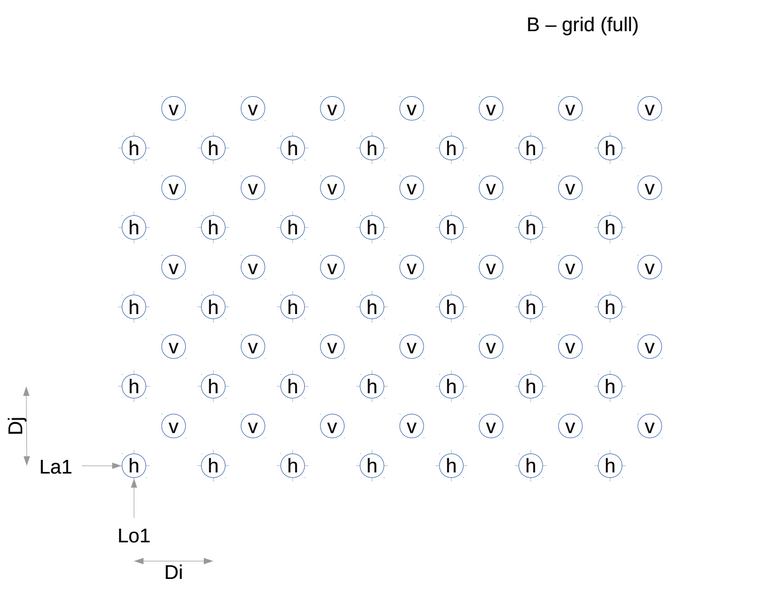
\includegraphics[width=4.22917in,height=2.13889in]{../tex/extracted-media/media/image1.emf}

\textbf{Class 06 -- BUFR/CREX Location (horizontal -- 2)}

\begin{longtable}[]{@{}lllllllll@{}}
\toprule
& & BUFR & CREX & & & & &\tabularnewline
\midrule
\endhead
TABLE & & & & & DATA & & & DATA\tabularnewline
REFERENCE & ELEMENT NAME & UNIT & SCALE & REFERENCE & WIDTH & UNIT & SCALE & WIDTH\tabularnewline
F X Y & & & & VALUE & (Bits) & & & (Characters)\tabularnewline
0 06 001 & Longitude (high accuracy) & ° & 5 & --18000000 & 26 & ° & 5 & 8\tabularnewline
0 06 002 & Longitude (coarse accuracy) & ° & 2 & --18000 & 16 & ° & 2 & 5\tabularnewline
0 06 011 & Longitude increment (high accuracy) & ° & 5 & --18000000 & 26 & ° & 5 & 8\tabularnewline
0 06 012 & Longitude increment (coarse accuracy) & ° & 2 & --18000 & 16 & ° & 2 & 5\tabularnewline
0 06 015 & Longitude displacement (high accuracy) & ° & 5 & --18000000 & 26 & ° & 5 & 8\tabularnewline
0 06 016 & Longitude displacement (coarse accuracy) & ° & 2 & --18000 & 16 & ° & 2 & 5\tabularnewline
0 06 021 & Distance & m & --1 & 0 & 13 & m & --1 & 4\tabularnewline
0 06 029 & Wave number & m\textsuperscript{--1} & 1 & 0 & 22 & m\textsuperscript{--1} & 1 & 7\tabularnewline
0 06 030 & Wave number (spectral) & rad m\textsuperscript{--1} & 5 & 0 & 13 & rad m\textsuperscript{--1} & 5 & 4\tabularnewline
0 06 031 & Column number & Numeric & 0 & 0 & 12 & Numeric & 0 & 4\tabularnewline
0 06 032 & X offset (see Note 6) & m & 2 & --1073741824 & 31 & m & 2 & 11\tabularnewline
0 06 033 & Pixel size on horizontal -- 2 & m & --1 & 0 & 16 & m & --1 & 5\tabularnewline
0 06 034 & Cross-track cell number & Numeric & 0 & 0 & 7 & Numeric & 0 & 3\tabularnewline
0 06 035 & Maximum size of y-dimension & Numeric & 0 & 0 & 12 & Numeric & 0 & 4\tabularnewline
0 06 040 & Radius of confidence & m & 0 & 0 & 13 & m & 0 & 4\tabularnewline
\bottomrule
\end{longtable}

Notes:

(1) Values of longitude are limited to the range --180 degrees to +180 degrees.

(2) West longitude shall be assigned negative values.

(3) East to west increments shall be assigned negative values.

(4) Distance shall only be used with respect to a stated location and a bearing, azimuth or elevation; it shall not redefine that location.

(5) The pixel size on horizontal -- 2 is given at location where map scale factor is unity.

\emph{(continued)}

\emph{\\
(Class 06 -- continued)}

(6) X offset is the distance between the projection origin and the upper left corner of the upper left pixel in a map, as shown in the following diagram:

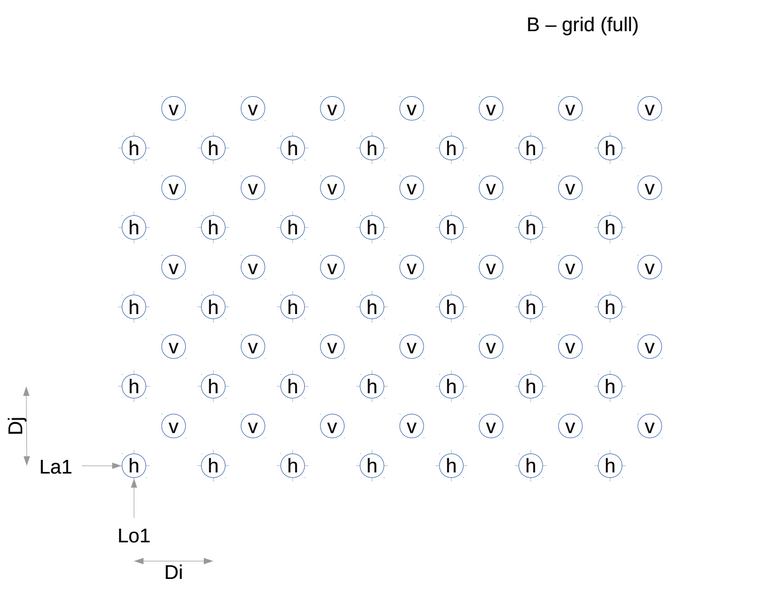
\includegraphics[width=4.37903in,height=2.0625in]{../tex/extracted-media/media/image1.emf}

\textbf{Class 07 -- BUFR/CREX Location (vertical)}

\begin{longtable}[]{@{}lllllllll@{}}
\toprule
& & BUFR & CREX & & & & &\tabularnewline
\midrule
\endhead
TABLE & & & & & DATA & & & DATA\tabularnewline
REFERENCE & ELEMENT NAME & UNIT & SCALE & REFERENCE & WIDTH & UNIT & SCALE & WIDTH\tabularnewline
F X Y & & & & VALUE & (Bits) & & & (Characters)\tabularnewline
0 07 001 & Height of station (see Note 1) & m & 0 & --400 & 15 & m & 0 & 5\tabularnewline
0 07 002 & Height or altitude & m & --1 & --40 & 16 & m & --1 & 5\tabularnewline
0 07 003 & Geopotential & m\textsuperscript{2} s\textsuperscript{--2} & --1 & --400 & 17 & m\textsuperscript{2} s\textsuperscript{--2} & --1 & 6\tabularnewline
0 07 004 & Pressure & Pa & --1 & 0 & 14 & Pa & --1 & 5\tabularnewline
0 07 005 & Height increment & m & 0 & --400 & 12 & m & 0 & 4\tabularnewline
0 07 006 & Height above station & m & 0 & 0 & 15 & m & 0 & 5\tabularnewline
0 07 007 & Height & m & 0 & --1000 & 17 & m & 0 & 6\tabularnewline
0 07 008 & Geopotential & m\textsuperscript{2} s\textsuperscript{--2} & 0 & --10000 & 20 & m\textsuperscript{2} s\textsuperscript{--2} & 0 & 7\tabularnewline
0 07 009 & Geopotential height & gpm & 0 & --1000 & 17 & gpm & 0 & 5\tabularnewline
0 07 010 & Flight level & m & 0 & --1024 & 16 & ft & --1 & 5\tabularnewline
0 07 012 & Grid point altitude & m & 2 & --50000 & 20 & m & 2 & 7\tabularnewline
0 07 021 & Elevation (see Note 2) & ° & 2 & --9000 & 15 & ° & 2 & 5\tabularnewline
0 07 022 & Solar elevation & ° & 2 & --9000 & 15 & ° & 2 & 5\tabularnewline
0 07 024 & Satellite zenith angle & ° & 2 & --9000 & 15 & ° & 2 & 5\tabularnewline
0 07 025 & Solar zenith angle & ° & 2 & --9000 & 15 & ° & 2 & 5\tabularnewline
0 07 026 & Satellite zenith angle & ° & 4 & --900000 & 21 & ° & 4 & 7\tabularnewline
0 07 030 & \vtop{\hbox{\strut Height of station ground above}\hbox{\strut mean sea level (see Note 3)}} & m & 1 & --4000 & 17 & m & 1 & 5\tabularnewline
0 07 031 & \vtop{\hbox{\strut Height of barometer above mean}\hbox{\strut sea level (see Note 4)}} & m & 1 & --4000 & 17 & m & 1 & 5\tabularnewline
\begin{minipage}[t]{0.08\columnwidth}\raggedright
0 07 032\strut
\end{minipage} & \begin{minipage}[t]{0.08\columnwidth}\raggedright
Height of sensor above local ground

(or deck of marine platform)

(see Note 5)\strut
\end{minipage} & \begin{minipage}[t]{0.08\columnwidth}\raggedright
m\strut
\end{minipage} & \begin{minipage}[t]{0.08\columnwidth}\raggedright
2\strut
\end{minipage} & \begin{minipage}[t]{0.08\columnwidth}\raggedright
0\strut
\end{minipage} & \begin{minipage}[t]{0.08\columnwidth}\raggedright
16\strut
\end{minipage} & \begin{minipage}[t]{0.08\columnwidth}\raggedright
m\strut
\end{minipage} & \begin{minipage}[t]{0.08\columnwidth}\raggedright
2\strut
\end{minipage} & \begin{minipage}[t]{0.08\columnwidth}\raggedright
5\strut
\end{minipage}\tabularnewline
0 07 033 & Height of sensor above water surface (see Note 6) & m & 1 & 0 & 12 & m & 1 & 4\tabularnewline
0 07 035 & Maximum size of z-dimension & Numeric & 0 & 0 & 12 & Numeric & 0 & 4\tabularnewline
\bottomrule
\end{longtable}

\emph{(continued)}

\emph{\\
(Class 07 -- continued)}

\begin{longtable}[]{@{}lllllllll@{}}
\toprule
& & BUFR & CREX & & & & &\tabularnewline
\midrule
\endhead
TABLE & & & & & DATA & & & DATA\tabularnewline
REFERENCE & ELEMENT NAME & UNIT & SCALE & REFERENCE & WIDTH & UNIT & SCALE & WIDTH\tabularnewline
F X Y & & & & VALUE & (Bits) & & & (Characters)\tabularnewline
0 07 036 & Level index of z & Numeric & 0 & 0 & 12 & Numeric & 0 & 4\tabularnewline
0 07 040 & Impact parameter (see Note 7) & m & 1 & 62000000 & 22 & m & 1 & 8\tabularnewline
0 07 061 & Depth below land surface & m & 2 & 0 & 14 & m & 2 & 5\tabularnewline
0 07 062 & Depth below sea/water surface & m & 1 & 0 & 17 & m & 1 & 6\tabularnewline
0 07 063 & Depth below sea/water surface (cm) & m & 2 & 0 & 20 & m & 2 & 7\tabularnewline
\begin{minipage}[t]{0.08\columnwidth}\raggedright
0 07 064\strut
\end{minipage} & \begin{minipage}[t]{0.08\columnwidth}\raggedright
Representative height of sensor

above station (see Note 8)\strut
\end{minipage} & \begin{minipage}[t]{0.08\columnwidth}\raggedright
m\strut
\end{minipage} & \begin{minipage}[t]{0.08\columnwidth}\raggedright
0\strut
\end{minipage} & \begin{minipage}[t]{0.08\columnwidth}\raggedright
0\strut
\end{minipage} & \begin{minipage}[t]{0.08\columnwidth}\raggedright
4\strut
\end{minipage} & \begin{minipage}[t]{0.08\columnwidth}\raggedright
m\strut
\end{minipage} & \begin{minipage}[t]{0.08\columnwidth}\raggedright
0\strut
\end{minipage} & \begin{minipage}[t]{0.08\columnwidth}\raggedright
2\strut
\end{minipage}\tabularnewline
0 07 065 & Water pressure & Pa & --3 & 0 & 17 & Pa & --3 & 6\tabularnewline
0 07 070 & Drogue depth & m & 0 & 0 & 10 & m & 0 & 4\tabularnewline
0 07 071 & Height (high resolution) & m & 3 & --10000000 & 26 & m & 3 & 8\tabularnewline
\bottomrule
\end{longtable}

Notes:

(1) Regarding data from ground-based stations, this descriptor should be used for archived data only. Descriptors 0 07 030 and 0 07 031 should be used and preferred to represent ground elevation and elevation of barometer, respectively, as defined in \emph{Weather Reporting} (WMO-No. 9), Volume A -- Observing Stations. Regarding marine stations, this descriptor refers to the height above mean sea level of the deck of marine platform where the instruments stand.

(2) Elevation shall only be used with respect to a stated location and a bearing, azimuth or distance; it shall not redefine that location.

(3) Height of station ground above mean sea level is defined as the height above mean sea level of the ground on which the raingauge stands or, if there is no raingauge, the ground beneath the thermometer screen. If there is neither raingauge nor screen, it is the average level of terrain in the vicinity of the station (Reference: \emph{Guide to Meteorological Instruments and Methods of Observation} (WMO-No. 8), 1996).

(4) Height of barometer above mean sea level, referring to the location of barometer of a station, does not redefine the descriptor 0 07 030.

(5) Height of sensor above local ground (or deck of marine platform) is the actual height of sensor above ground (or deck of marine platform) at the point where the sensor is located. This descriptor does not redefine the descriptors 0 07 030 or 0 07 033. Previously defined value of 0 07 032 may be cancelled by setting 0~07~032 to a "missing value".

(6) Height of sensor above water surface is the height of sensor above water surface of sea or lake. This descriptor does not redefine descriptors 0 07 030 or 0~07~032. Previously defined value 0 07 033 may be cancelled by setting 0 07 033 to a "missing value".

(7) For an atmospheric limb sounder, the ``impact parameter'' is the distance between the ray asymptote and the centre of curvature of the Earth's surface at the tangent point.

(8) Representative height of sensor above station is the standard height of a sensor required by WMO documentation. The value of the following meteorological element should be adjusted using a formula. For example, standard height recommended in WMO documentation for surface wind sensors is 10 metres. If the sensor is placed at a different height, the wind speed may be adjusted using a formula.

\textbf{Class 08 -- BUFR/CREX Significance qualifiers}

\begin{longtable}[]{@{}lllllllll@{}}
\toprule
& & BUFR & CREX & & & & &\tabularnewline
\midrule
\endhead
TABLE & & & & & DATA & & & DATA\tabularnewline
REFERENCE & ELEMENT NAME & UNIT & SCALE & REFERENCE & WIDTH & UNIT & SCALE & WIDTH\tabularnewline
F X Y & & & & VALUE & (Bits) & & & (Characters)\tabularnewline
0 08 001 & Vertical sounding significance & Flag table & 0 & 0 & 7 & Flag table & 0 & 3\tabularnewline
0 08 002 & Vertical significance (surface observations) & Code table & 0 & 0 & 6 & Code table & 0 & 2\tabularnewline
0 08 003 & Vertical significance (satellite observations) & Code table & 0 & 0 & 6 & Code table & 0 & 2\tabularnewline
0 08 004 & Phase of aircraft flight & Code table & 0 & 0 & 3 & Code table & 0 & 1\tabularnewline
0 08 005 & Meteorological attribute significance & Code table & 0 & 0 & 4 & Code table & 0 & 2\tabularnewline
0 08 006 & Ozone vertical sounding significance & Flag table & 0 & 0 & 9 & Flag table & 0 & 3\tabularnewline
0 08 007 & Dimensional significance & Code table & 0 & 0 & 4 & Code table & 0 & 2\tabularnewline
0 08 008 & \vtop{\hbox{\strut Radiation vertical sounding}\hbox{\strut significance}} & Flag table & 0 & 0 & 9 & Flag table & 0 & 3\tabularnewline
0 08 009 & Detailed phase of flight & Code table & 0 & 0 & 4 & Code table & 0 & 2\tabularnewline
0 08 010 & Surface qualifier (temperature data) & Code table & 0 & 0 & 5 & Code table & 0 & 2\tabularnewline
0 08 011 & Meteorological feature & Code table & 0 & 0 & 6 & Code table & 0 & 2\tabularnewline
0 08 012 & Land/sea qualifier & Code table & 0 & 0 & 2 & Code table & 0 & 1\tabularnewline
0 08 013 & Day/night qualifier & Code table & 0 & 0 & 2 & Code table & 0 & 1\tabularnewline
0 08 014 & Qualifier for runway visual range & Code table & 0 & 0 & 4 & Code table & 0 & 2\tabularnewline
0 08 015 & Significant qualifier for sensor & Code table & 0 & 0 & 3 & Code table & 0 & 1\tabularnewline
0 08 016 & \vtop{\hbox{\strut Change qualifier of a trend-type}\hbox{\strut forecast or an aerodrome forecast}} & Code table & 0 & 0 & 3 & Code table & 0 & 1\tabularnewline
0 08 017 & \vtop{\hbox{\strut Qualifier of the time when the}\hbox{\strut forecast change is expected}} & Code table & 0 & 0 & 2 & Code table & 0 & 1\tabularnewline
0 08 018 & SEAWINDS land/ice surface type & Flag table & 0 & 0 & 17 & Flag table & 0 & 6\tabularnewline
0 08 019 & Qualifier for following centre identifier & Code table & 0 & 0 & 4 & Code table & 0 & 2\tabularnewline
0 08 020 & \vtop{\hbox{\strut Total number of missing entities}\hbox{\strut (with respect to accumulation or average)}} & Numeric & 0 & 0 & 16 & Numeric & 0 & 5\tabularnewline
\bottomrule
\end{longtable}

\emph{(continued)}

\emph{\\
(Class 08 -- continued)}

\begin{longtable}[]{@{}lllllllll@{}}
\toprule
& & BUFR & CREX & & & & &\tabularnewline
\midrule
\endhead
TABLE & & & & & DATA & & & DATA\tabularnewline
REFERENCE & ELEMENT NAME & UNIT & SCALE & REFERENCE & WIDTH & UNIT & SCALE & WIDTH\tabularnewline
F X Y & & & & VALUE & (Bits) & & & (Characters)\tabularnewline
0 08 021 & Time significance & Code table & 0 & 0 & 5 & Code table & 0 & 2\tabularnewline
0 08 022 & Total number (with respect to accumulation or average) & Numeric & 0 & 0 & 16 & Numeric & 0 & 5\tabularnewline
0 08 023 & First-order statistics & Code table & 0 & 0 & 6 & Code table & 0 & 2\tabularnewline
0 08 024 & Difference statistics & Code table & 0 & 0 & 6 & Code table & 0 & 2\tabularnewline
0 08 025 & Time difference qualifier (see Note 5) & Code table & 0 & 0 & 4 & Code table & 0 & 2\tabularnewline
0 08 026 & Matrix significance & Code table & 0 & 0 & 6 & Code table & 0 & 2\tabularnewline
0 08 029 & Surface type & Code table & 0 & 0 & 8 & Code table & 0 & 3\tabularnewline
\begin{minipage}[t]{0.08\columnwidth}\raggedright
0 08 030\strut
\end{minipage} & \begin{minipage}[t]{0.08\columnwidth}\raggedright
\emph{Manual on Codes} (Volume I.1,

Section C) Code table from which

data are derived\strut
\end{minipage} & \begin{minipage}[t]{0.08\columnwidth}\raggedright
Numeric\strut
\end{minipage} & \begin{minipage}[t]{0.08\columnwidth}\raggedright
0\strut
\end{minipage} & \begin{minipage}[t]{0.08\columnwidth}\raggedright
0\strut
\end{minipage} & \begin{minipage}[t]{0.08\columnwidth}\raggedright
13\strut
\end{minipage} & \begin{minipage}[t]{0.08\columnwidth}\raggedright
Numeric\strut
\end{minipage} & \begin{minipage}[t]{0.08\columnwidth}\raggedright
0\strut
\end{minipage} & \begin{minipage}[t]{0.08\columnwidth}\raggedright
4\strut
\end{minipage}\tabularnewline
0 08 031 & Data category -- CREX table A & Numeric & 0 & 0 & 8 & Numeric & 0 & 3\tabularnewline
0 08 032 & Status of operation & Code table & 0 & 0 & 4 & Code table & 0 & 2\tabularnewline
0 08 033 & Method of derivation of percentage confidence (see Note 6) & Code table & 0 & 0 & 7 & Code table & 0 & 3\tabularnewline
0 08 034 & Temperature/salinity measurement qualifier & Code table & 0 & 0 & 4 & Code table & 0 & 2\tabularnewline
0 08 035 & Type of monitoring exercise & Code table & 0 & 0 & 3 & Code table & 0 & 1\tabularnewline
0 08 036 & Type of centre or station performing monitoring & Code table & 0 & 0 & 3 & Code table & 0 & 1\tabularnewline
0 08 037 & Baseline check significance & Code table & 0 & 0 & 5 & Code table & 0 & 2\tabularnewline
0 08 038 & Instrument data significance & Code table & 0 & 0 & 8 & Code table & 0 & 3\tabularnewline
0 08 039 & Time significance (Aviation forecast) & Code table & 0 & 0 & 6 & Code table & 0 & 2\tabularnewline
0 08 040 & Flight level significance & Code table & 0 & 0 & 6 & Code table & 0 & 2\tabularnewline
0 08 041 & Data significance & Code table & 0 & 0 & 5 & Code table & 0 & 2\tabularnewline
\bottomrule
\end{longtable}

\emph{(continued)}

\emph{\\
(Class 08 -- continued)}

\begin{longtable}[]{@{}lllllllll@{}}
\toprule
& & BUFR & CREX & & & & &\tabularnewline
\midrule
\endhead
TABLE & & & & & DATA & & & DATA\tabularnewline
REFERENCE & ELEMENT NAME & UNIT & SCALE & REFERENCE & WIDTH & UNIT & SCALE & WIDTH\tabularnewline
F X Y & & & & VALUE & (Bits) & & & (Characters)\tabularnewline
0 08 042 & Extended vertical sounding significance & Flag table & 0 & 0 & 18 & Flag table & 0 & 6\tabularnewline
0 08 043 & Atmospheric chemical or physical constituent type & Code table & 0 & 0 & 8 & Code table & 0 & 3\tabularnewline
0 08 044 & CAS registry number & CCITT IA5 & 0 & 0 & 88 & Character & 0 & 11\tabularnewline
0 08 046 & Atmospheric chemical or physical constituent type & Common Code table C--14 & 0 & 0 & 16 & Common Code table C--14 & 0 & 5\tabularnewline
0 08 049 & Number of observations & Numeric & 0 & 0 & 8 & Numeric & 0 & 3\tabularnewline
0 08 050 & \vtop{\hbox{\strut Qualifier for number of missing}\hbox{\strut values in calculation of statistic}} & Code table & 0 & 0 & 4 & Code table & 0 & 2\tabularnewline
0 08 051 & \vtop{\hbox{\strut Qualifier for number of missing}\hbox{\strut values in calculation of statistic}} & Code table & 0 & 0 & 3 & Code table & 0 & 1\tabularnewline
0 08 052 & \vtop{\hbox{\strut Condition for which number of days}\hbox{\strut of occurrence follows}} & Code table & 0 & 0 & 5 & Code table & 0 & 2\tabularnewline
0 08 053 & Day of occurrence qualifier & Code table & 0 & 0 & 2 & Code table & 0 & 1\tabularnewline
0 08 054 & Qualifier for wind speed or wind gusts & Code table & 0 & 0 & 3 & Code table & 0 & 1\tabularnewline
0 08 060 & Sample scanning mode significance & Code table & 0 & 0 & 4 & Code table & 0 & 2\tabularnewline
0 08 065 & Sun-glint indicator & Code table & 0 & 0 & 2 & Code table & 0 & 1\tabularnewline
0 08 066 & Semi-transparency indicator & Code table & 0 & 0 & 2 & Code table & 0 & 1\tabularnewline
0 08 070 & Vertical sounding product qualifier & Code table & 0 & 0 & 4 & Code table & 0 & 2\tabularnewline
0 08 072 & Pixel(s) type & Code table & 0 & 0 & 3 & Code table & 0 & 1\tabularnewline
0 08 074 & Altimeter echo type & Code table & 0 & 0 & 2 & Code table & 0 & 1\tabularnewline
0 08 075 & Ascending/descending orbit qualifier & Code table & 0 & 0 & 2 & Code table & 0 & 1\tabularnewline
0 08 076 & Type of band & Code table & 0 & 0 & 6 & Code table & 0 & 2\tabularnewline
0 08 077 & Radiometer sensed surface type & Code table & 0 & 0 & 7 & Code table & 0 & 3\tabularnewline
0 08 079 & Product status & Code table & 0 & 0 & 4 & Code table & 0 & 2\tabularnewline
0 08 080 & Qualifier for GTSPP quality flag & Code table & 0 & 0 & 6 & Code table & 0 & 2\tabularnewline
\bottomrule
\end{longtable}

\emph{(continued)}

\emph{\\
(Class 08 -- continued)}

\begin{longtable}[]{@{}lllllllll@{}}
\toprule
& & BUFR & CREX & & & & &\tabularnewline
\midrule
\endhead
TABLE & & & & & DATA & & & DATA\tabularnewline
REFERENCE & ELEMENT NAME & UNIT & SCALE & REFERENCE & WIDTH & UNIT & SCALE & WIDTH\tabularnewline
F X Y & & & & VALUE & (Bits) & & & (Characters)\tabularnewline
0 08 081 & Type of equipment & Code table & 0 & 0 & 6 & Code table & 0 & 2\tabularnewline
0 08 082 & \vtop{\hbox{\strut Modification of sensor height}\hbox{\strut to another value}} & Code table & 0 & 0 & 3 & Code table & 0 & 1\tabularnewline
0 08 083 & Nominal value indicator & Flag table & 0 & 0 & 15 & Flag table & 0 & 5\tabularnewline
0 08 085 & Beam identifier & Code table & 0 & 0 & 3 & Code table & 0 & 1\tabularnewline
0 08 086 & Vertical significance for NWP & Flag table & 0 & 0 & 12 & Flag table & 0 & 4\tabularnewline
0 08 087 & Corner position of observation & Code table & 0 & 0 & 3 & Code table & 0 & 1\tabularnewline
0 08 088 & Map significance & Code table & \textbf{0} & \textbf{0} & \textbf{6} & \textbf{Code table} & \textbf{0} & \textbf{2}\tabularnewline
0 08 090 & \vtop{\hbox{\strut Decimal scale of following}\hbox{\strut significands}} & Numeric & 0 & --127 & 8 & Numeric & 0 & 3\tabularnewline
0 08 091 & Coordinates significance & Code table & 0 & 0 & 8 & Code table & 0 & 3\tabularnewline
0 08 092 & Measurement uncertainty expression & Code table & 0 & 0 & 5 & Code table & 0 & 2\tabularnewline
0 08 093 & Measurement uncertainty significance & Code table & 0 & 0 & 5 & Code table & 0 & 2\tabularnewline
\bottomrule
\end{longtable}

Notes:

(1) Where values are accumulated or averaged (for example over a time period), the total number of values from which the accumulated or averaged values are obtained may be represented using reference 0 08 022.

(2) A previously defined significance may be cancelled by transmitting a ``missing'' from the appropriate code or flag table.

(3) First-order statistics have values with a similar range and the same dimensions as the corresponding reported values (e.g., maxima, minima, means).

(4) Difference statistics are difference values; they have dimensions similar to the corresponding reported values with respect to units, but assume a range centred on zero (e.g. the difference between reported and analysed values, the difference between reported and forecast values).

(5) Descriptor 0 08 025 is to be used with 0 26 003 (time difference).

(6) Descriptor 0 08 033 is to be used by preceding the element 0 33 007 as part of quality control information in order to specify the method used to calculate the percentage confidence.

\emph{(continued)}

\emph{\\
(Class 08 -- continued)}

(7) When descriptor 0~08~043 is used to specify particulate matter (PM) under a given size threshold, descriptor 0~08~045 may also be used to further specify a subset of the PM population on the basis of ion composition.

(8) Descriptor 0 08 090 is to be used to establish the decimal scale of one or more subsequent numerical element descriptors requiring a large dynamic range of values. The numerical element descriptor(s) will contain the scaled value of the measurement(s) with the required number of significant digits. The actual value will be obtained, at the application level, by multiplying the scaled value by the given decimal scale: (scaled value x 10\textsuperscript{decimal scale}).

\textbf{Class 10 -- BUFR/CREX Non-coordinate location (vertical)}

\begin{longtable}[]{@{}lllllllll@{}}
\toprule
& & BUFR & CREX & & & & &\tabularnewline
\midrule
\endhead
TABLE & & & & & DATA & & & DATA\tabularnewline
REFERENCE & ELEMENT NAME & UNIT & SCALE & REFERENCE & WIDTH & UNIT & SCALE & WIDTH\tabularnewline
F X Y & & & & VALUE & (Bits) & & & (Characters)\tabularnewline
0 10 001 & Height of land surface & m & 0 & --400 & 15 & m & 0 & 5\tabularnewline
0 10 002 & Height & m & --1 & --40 & 16 & m & --1 & 5\tabularnewline
0 10 003 & Geopotential & m\textsuperscript{2} s\textsuperscript{--2} & --1 & --400 & 17 & m\textsuperscript{2} s\textsuperscript{--2} & --1 & 6\tabularnewline
0 10 004 & Pressure & Pa & --1 & 0 & 14 & Pa & --1 & 5\tabularnewline
0 10 007 & Height & m & 0 & --1000 & 17 & m & 0 & 6\tabularnewline
0 10 008 & Geopotential & m\textsuperscript{2} s\textsuperscript{--2} & 0 & --10000 & 20 & m\textsuperscript{2} s\textsuperscript{--2} & 0 & 7\tabularnewline
0 10 009 & Geopotential height & gpm & 0 & --1000 & 17 & gpm & 0 & 5\tabularnewline
\begin{minipage}[t]{0.08\columnwidth}\raggedright
0 10 010\strut
\end{minipage} & \begin{minipage}[t]{0.08\columnwidth}\raggedright
Minimum pressure reduced to

mean sea level\strut
\end{minipage} & \begin{minipage}[t]{0.08\columnwidth}\raggedright
Pa\strut
\end{minipage} & \begin{minipage}[t]{0.08\columnwidth}\raggedright
--1\strut
\end{minipage} & \begin{minipage}[t]{0.08\columnwidth}\raggedright
0\strut
\end{minipage} & \begin{minipage}[t]{0.08\columnwidth}\raggedright
14\strut
\end{minipage} & \begin{minipage}[t]{0.08\columnwidth}\raggedright
Pa\strut
\end{minipage} & \begin{minipage}[t]{0.08\columnwidth}\raggedright
--1\strut
\end{minipage} & \begin{minipage}[t]{0.08\columnwidth}\raggedright
5\strut
\end{minipage}\tabularnewline
\begin{minipage}[t]{0.08\columnwidth}\raggedright
0 10 011\strut
\end{minipage} & \begin{minipage}[t]{0.08\columnwidth}\raggedright
Maximum pressure reduced to

mean sea level\strut
\end{minipage} & \begin{minipage}[t]{0.08\columnwidth}\raggedright
Pa\strut
\end{minipage} & \begin{minipage}[t]{0.08\columnwidth}\raggedright
--1\strut
\end{minipage} & \begin{minipage}[t]{0.08\columnwidth}\raggedright
0\strut
\end{minipage} & \begin{minipage}[t]{0.08\columnwidth}\raggedright
14\strut
\end{minipage} & \begin{minipage}[t]{0.08\columnwidth}\raggedright
Pa\strut
\end{minipage} & \begin{minipage}[t]{0.08\columnwidth}\raggedright
--1\strut
\end{minipage} & \begin{minipage}[t]{0.08\columnwidth}\raggedright
5\strut
\end{minipage}\tabularnewline
\begin{minipage}[t]{0.08\columnwidth}\raggedright
0 10 031\strut
\end{minipage} & \begin{minipage}[t]{0.08\columnwidth}\raggedright
In direction of the North Pole,

distance from the Earth's centre

(see Notes 2 and 3)\strut
\end{minipage} & \begin{minipage}[t]{0.08\columnwidth}\raggedright
m\strut
\end{minipage} & \begin{minipage}[t]{0.08\columnwidth}\raggedright
2\strut
\end{minipage} & \begin{minipage}[t]{0.08\columnwidth}\raggedright
--1073741824\strut
\end{minipage} & \begin{minipage}[t]{0.08\columnwidth}\raggedright
31\strut
\end{minipage} & \begin{minipage}[t]{0.08\columnwidth}\raggedright
m\strut
\end{minipage} & \begin{minipage}[t]{0.08\columnwidth}\raggedright
2\strut
\end{minipage} & \begin{minipage}[t]{0.08\columnwidth}\raggedright
10\strut
\end{minipage}\tabularnewline
0 10 032 & Satellite distance to Earth's centre & m & 1 & 0 & 27 & m & 2 & 9\tabularnewline
0 10 033 & Altitude (platform to ellipsoid) & m & 1 & 0 & 27 & m & 2 & 9\tabularnewline
0 10 034 & Earth's radius & m & 1 & 0 & 27 & m & 2 & 9\tabularnewline
0 10 035 & Earth's local radius of curvature & m & 1 & 62000000 & 22 & m & 1 & 8\tabularnewline
0 10 036 & Geoid undulation (see Note 4) & m & 2 & --15000 & 15 & m & 2 & 6\tabularnewline
0 10 038 & Maximum height of deck cargo above summer load line & m & 0 & 0 & 6 & m & 0 & 2\tabularnewline
0 10 039 & Departure of reference level (summer maximum load line) from actual sea level & m & 0 & --32 & 6 & m & 0 & 3\tabularnewline
0 10 040 & Number of retrieved layers & Numeric & 0 & 0 & 10 & Numeric & 0 & 4\tabularnewline
0 10 050 & Standard deviation altitude & m & 2 & 0 & 16 & m & 2 & 5\tabularnewline
0 10 051 & Pressure reduced to mean sea level & Pa & --1 & 0 & 14 & Pa & --1 & 5\tabularnewline
\bottomrule
\end{longtable}

\emph{(continued)}

\emph{\\
(Class 10 -- continued)}

\begin{longtable}[]{@{}lllllllll@{}}
\toprule
& & BUFR & CREX & & & & &\tabularnewline
\midrule
\endhead
TABLE & & & & & DATA & & & DATA\tabularnewline
REFERENCE & ELEMENT NAME & UNIT & SCALE & REFERENCE & WIDTH & UNIT & SCALE & WIDTH\tabularnewline
F X Y & & & & VALUE & (Bits) & & & (Characters)\tabularnewline
0 10 052 & Altimeter setting (QNH) & Pa & --1 & 0 & 14 & Pa & --1 & 5\tabularnewline
0 10 053 & Global navigation satellite system altitude & m & 0 & --1000 & 17 & m & 0 & 5\tabularnewline
0 10 060 & Pressure change & Pa & --1 & --1024 & 11 & Pa & --1 & 4\tabularnewline
0 10 061 & 3-hour pressure change & Pa & --1 & --500 & 10 & Pa & --1 & 4\tabularnewline
0 10 062 & 24-hour pressure change & Pa & --1 & --1000 & 11 & Pa & --1 & 4\tabularnewline
0 10 063 & Characteristic of pressure tendency & Code table & 0 & 0 & 4 & Code table & 0 & 2\tabularnewline
0 10 064 & SIGMET cruising level & Code table & 0 & 0 & 3 & Code table & 0 & 1\tabularnewline
0 10 070 & Indicated aircraft altitude & m & 0 & --400 & 16 & m & 0 & 5\tabularnewline
0 10 071 & Vertical resolution & m & 0 & 0 & 14 & m & 0 & 5\tabularnewline
0 10 079 & Off-nadir angle of the satellite from platform data & ° & 4 & 0 & 16 & ° & 4 & 5\tabularnewline
0 10 080 & Viewing zenith angle & ° & 2 & --9000 & 15 & ° & 2 & 5\tabularnewline
0 10 081 & Altitude of COG above reference ellipsoid & m & 3 & 0 & 31 & m & 3 & 10\tabularnewline
0 10 082 & Instantaneous altitude rate & m s\textsuperscript{--1} & 3 & --65536 & 17 & m s\textsuperscript{--1} & 3 & 6\tabularnewline
0 10 083 & \vtop{\hbox{\strut Squared off-nadir angle of the}\hbox{\strut satellite from platform data}} & degree\textsuperscript{2} & 2 & 0 & 16 & degree\textsuperscript{2} & 2 & 5\tabularnewline
0 10 084 & \vtop{\hbox{\strut Squared off-nadir angle of the}\hbox{\strut satellite from waveform data}} & degree\textsuperscript{2} & 2 & 0 & 16 & degree\textsuperscript{2} & 2 & 5\tabularnewline
0 10 085 & Mean sea-surface height & m & 3 & --131072 & 18 & m & 3 & 6\tabularnewline
0 10 086 & Geoid's height & m & 3 & --131072 & 18 & m & 3 & 6\tabularnewline
0 10 087 & Ocean depth/land elevation & m & 1 & --131072 & 18 & m & 1 & 6\tabularnewline
0 10 088 & \vtop{\hbox{\strut Total geocentric ocean tide}\hbox{\strut height (solution 1)}} & m & 3 & --32768 & 16 & m & 3 & 5\tabularnewline
\bottomrule
\end{longtable}

\emph{(continued)}

\emph{\\
(Class 10 -- continued)}

\begin{longtable}[]{@{}lllllllll@{}}
\toprule
& & BUFR & CREX & & & & &\tabularnewline
\midrule
\endhead
TABLE & & & & & DATA & & & DATA\tabularnewline
REFERENCE & ELEMENT NAME & UNIT & SCALE & REFERENCE & WIDTH & UNIT & SCALE & WIDTH\tabularnewline
F X Y & & & & VALUE & (Bits) & & & (Characters)\tabularnewline
0 10 089 & \vtop{\hbox{\strut Total geocentric ocean tide}\hbox{\strut height (solution 2)}} & m & 3 & --32768 & 16 & m & 3 & 5\tabularnewline
0 10 090 & Long period tide height & m & 3 & --32768 & 16 & m & 3 & 5\tabularnewline
0 10 091 & Tidal loading height & m & 3 & --32768 & 16 & m & 3 & 5\tabularnewline
0 10 092 & Solid Earth tide height & m & 3 & --32768 & 16 & m & 3 & 5\tabularnewline
0 10 093 & Geocentric pole tide height & m & 3 & --32768 & 16 & m & 3 & 5\tabularnewline
0 10 095 & Height of atmosphere used & m & 0 & 0 & 16 & m & 0 & 5\tabularnewline
0 10 096 & Mean dynamic topography & m & 3 & --131072 & 18 & m & 3 & 6\tabularnewline
0 10 097 & \vtop{\hbox{\strut Mean sea-surface height from}\hbox{\strut altimeter only}} & m & 3 & --131072 & 18 & m & 3 & 6\tabularnewline
0 10 098 & \vtop{\hbox{\strut Loading tide height geocentric}\hbox{\strut ocean tide solution 1}} & m & 4 & --2000 & 12 & m & 4 & 4\tabularnewline
0 10 099 & \vtop{\hbox{\strut Loading tide height geocentric}\hbox{\strut ocean tide solution 2}} & m & 4 & --2000 & 12 & m & 4 & 4\tabularnewline
0 10 100 & \vtop{\hbox{\strut Non-equilibrium long period}\hbox{\strut tide height}} & m & 4 & --2000 & 12 & m & 4 & 4\tabularnewline
0 10 101 & \vtop{\hbox{\strut Squared off-nadir angle of the}\hbox{\strut satellite from waveform data}} & degree\textsuperscript{2} & 2 & --32768 & 16 & degree\textsuperscript{2} & 2 & 5\tabularnewline
0 10 102 & Sea-surface height anomaly & m & 3 & --32768 & 16 & m & 3 & 5\tabularnewline
0 10 103 & Mean dynamic topography accuracy & m & 3 & --131072 & 18 & m & 3 & 6\tabularnewline
\bottomrule
\end{longtable}

Notes:

(1) Vertical elements and pressure shall be used to define values of these elements independent of the element or variable denoting the vertical coordinate.

(2) The value for descriptor 0 10 031 has been chosen to be suitable for polar orbiting satellites in approximately Sun-synchronous orbits. Geostationary orbits would require greater data widths for distance and slightly less for speed.

(3) Left handed x, y and z axes have been chosen for descriptor 0 10 031.

(4) The ``geoid undulation'' is the difference between the reference ellipsoid (WGS-84) and the geoid height (EGM96) at the geographic location of the observation, both referenced to the centre of mass of the Earth.

\textbf{Class 11 -- BUFR/CREX Wind and turbulence}

\begin{longtable}[]{@{}lllllllll@{}}
\toprule
& & BUFR & CREX & & & & &\tabularnewline
\midrule
\endhead
TABLE & & & & & DATA & & & DATA\tabularnewline
REFERENCE & ELEMENT NAME & UNIT & SCALE & REFERENCE & WIDTH & UNIT & SCALE & WIDTH\tabularnewline
F X Y & & & & VALUE & (Bits) & & & (Characters)\tabularnewline
0 11 001 & Wind direction & degree true & 0 & 0 & 9 & degree true & 0 & 3\tabularnewline
0 11 002 & Wind speed & m s\textsuperscript{--1} & 1 & 0 & 12 & m s\textsuperscript{--1} & 1 & 4\tabularnewline
0 11 003 & u-component & m s\textsuperscript{--1} & 1 & --4096 & 13 & m s\textsuperscript{--1} & 1 & 4\tabularnewline
0 11 004 & v-component & m s\textsuperscript{--1} & 1 & --4096 & 13 & m s\textsuperscript{--1} & 1 & 4\tabularnewline
0 11 005 & w-component & Pa s\textsuperscript{--1} & 1 & --512 & 10 & Pa s\textsuperscript{--1} & 1 & 4\tabularnewline
0 11 006 & w-component & m s\textsuperscript{--1} & 2 & --4096 & 13 & m s\textsuperscript{--1} & 2 & 4\tabularnewline
0 11 007 & Relative wind direction (in degrees off bow) & ° & 0 & 0 & 9 & ° & 0 & 3\tabularnewline
0 11 008 & Relative wind speed & m s\textsuperscript{--1} & 1 & 0 & 12 & m s\textsuperscript{--1} & 1 & 4\tabularnewline
0 11 010 & Wind direction associated with wind speed which follows & degree true & 0 & 0 & 9 & degree true & 0 & 3\tabularnewline
0 11 011 & Wind direction at 10 m & degree true & 0 & 0 & 9 & degree true & 0 & 3\tabularnewline
0 11 012 & Wind speed at 10 m & m s\textsuperscript{--1} & 1 & 0 & 12 & m s\textsuperscript{--1} & 1 & 4\tabularnewline
0 11 013 & Wind direction at 5 m & degree true & 0 & 0 & 9 & degree true & 0 & 3\tabularnewline
0 11 014 & Wind speed at 5 m & m s\textsuperscript{--1} & 1 & 0 & 12 & m s\textsuperscript{--1} & 1 & 4\tabularnewline
0 11 016 & Extreme counterclockwise wind direction of a variable wind & degree true & 0 & 0 & 9 & degree true & 0 & 3\tabularnewline
0 11 017 & \vtop{\hbox{\strut Extreme clockwise wind direction of}\hbox{\strut a variable wind}} & degree true & 0 & 0 & 9 & degree true & 0 & 3\tabularnewline
0 11 019 & Steadiness of wind (see Note 6) & \% & 0 & 0 & 7 & \% & 0 & 3\tabularnewline
0 11 021 & Relative vorticity & s\textsuperscript{--1} & 9 & --65536 & 17 & s\textsuperscript{--1} & 9 & 6\tabularnewline
0 11 022 & Divergence & s\textsuperscript{--1} & 9 & --65536 & 17 & s\textsuperscript{--1} & 9 & 6\tabularnewline
0 11 023 & Velocity potential & m\textsuperscript{2} s\textsuperscript{--1} & --2 & --65536 & 17 & m\textsuperscript{2} s\textsuperscript{--1} & --2 & 6\tabularnewline
0 11 030 & Extended degree of turbulence & Code table & 0 & 0 & 6 & Code table & 0 & 2\tabularnewline
0 11 031 & Degree of turbulence & Code table & 0 & 0 & 4 & Code table & 0 & 2\tabularnewline
\bottomrule
\end{longtable}

\emph{(continued)}

\emph{\\
(Class 11 -- continued)}

\begin{longtable}[]{@{}lllllllll@{}}
\toprule
& & BUFR & CREX & & & & &\tabularnewline
\midrule
\endhead
TABLE & & & & & DATA & & & DATA\tabularnewline
REFERENCE & ELEMENT NAME & UNIT & SCALE & REFERENCE & WIDTH & UNIT & SCALE & WIDTH\tabularnewline
F X Y & & & & VALUE & (Bits) & & & (Characters)\tabularnewline
0 11 032 & Height of base of turbulence & m & --1 & --40 & 16 & m & --1 & 5\tabularnewline
0 11 033 & Height of top of turbulence & m & --1 & --40 & 16 & m & --1 & 5\tabularnewline
0 11 034 & Vertical gust velocity & m s\textsuperscript{--1} & 1 & --1024 & 11 & m s\textsuperscript{--1} & 1 & 4\tabularnewline
0 11 035 & Vertical gust acceleration & m s\textsuperscript{--2} & 2 & --8192 & 14 & m s\textsuperscript{--2} & 2 & 5\tabularnewline
0 11 036 & \vtop{\hbox{\strut Maximum derived equivalent}\hbox{\strut vertical gust speed}} & m s\textsuperscript{--1} & 1 & 0 & 10 & m s\textsuperscript{--1} & 1 & 4\tabularnewline
0 11 037 & Turbulence index & Code table & 0 & 0 & 6 & Code table & 0 & 2\tabularnewline
0 11 038 & Time of occurrence of peak eddy dissipation rate & Code table & 0 & 0 & 5 & Code table & 0 & 2\tabularnewline
0 11 039 & \vtop{\hbox{\strut Extended time of occurrence of}\hbox{\strut peak eddy dissipation rate}} & Code table & 0 & 0 & 6 & Code table & 0 & 2\tabularnewline
0 11 040 & Maximum wind speed (mean wind) & m s\textsuperscript{--1} & 1 & 0 & 12 & m s\textsuperscript{--1} & 1 & 4\tabularnewline
0 11 041 & Maximum wind gust speed & m s\textsuperscript{--1} & 1 & 0 & 12 & m s\textsuperscript{--1} & 1 & 4\tabularnewline
0 11 042 & \vtop{\hbox{\strut Maximum wind speed (10-minute}\hbox{\strut mean wind)}} & m s\textsuperscript{--1} & 1 & 0 & 12 & m s\textsuperscript{--1} & 1 & 4\tabularnewline
0 11 043 & Maximum wind gust direction & degree true & 0 & 0 & 9 & degree true & 0 & 3\tabularnewline
0 11 044 & \vtop{\hbox{\strut Mean wind direction for surface --}\hbox{\strut 1 500 m (5 000 feet)}} & degree true & 0 & 0 & 9 & degree true & 0 & 3\tabularnewline
0 11 045 & \vtop{\hbox{\strut Mean wind speed for surface --}\hbox{\strut 1 500 m (5 000 feet)}} & m s\textsuperscript{--1} & 1 & 0 & 12 & m s\textsuperscript{--1} & 1 & 4\tabularnewline
0 11 046 & Maximum instantaneous wind speed & m s\textsuperscript{--1} & 1 & 0 & 12 & m s\textsuperscript{--1} & 1 & 4\tabularnewline
0 11 047 & Maximum instantaneous wind speed over 10 minutes & m s\textsuperscript{--1} & 1 & 0 & 12 & m s\textsuperscript{--1} & 1 & 4\tabularnewline
0 11 049 & Standard deviation of wind direction & degree true & 0 & 0 & 9 & degree true & 0 & 3\tabularnewline
0 11 050 & \vtop{\hbox{\strut Standard deviation of horizontal}\hbox{\strut wind speed}} & m s\textsuperscript{--1} & 1 & 0 & 12 & m s\textsuperscript{--1} & 1 & 4\tabularnewline
\bottomrule
\end{longtable}

\emph{(continued)}

\emph{\\
(Class 11 -- continued)}

\begin{longtable}[]{@{}lllllllll@{}}
\toprule
& & BUFR & CREX & & & & &\tabularnewline
\midrule
\endhead
TABLE & & & & & DATA & & & DATA\tabularnewline
REFERENCE & ELEMENT NAME & UNIT & SCALE & REFERENCE & WIDTH & UNIT & SCALE & WIDTH\tabularnewline
F X Y & & & & VALUE & (Bits) & & & (Characters)\tabularnewline
0 11 051 & \vtop{\hbox{\strut Standard deviation of vertical}\hbox{\strut wind speed}} & m s\textsuperscript{--1} & 1 & 0 & 8 & m s\textsuperscript{--1} & 1 & 3\tabularnewline
0 11 052 & Formal uncertainty in wind speed & m s\textsuperscript{--1} & 2 & 0 & 13 & m s\textsuperscript{--1} & 2 & 5\tabularnewline
0 11 053 & Formal uncertainty in wind direction & degree true & 2 & 0 & 15 & degree true & 2 & 5\tabularnewline
0 11 054 & Mean wind direction for 1 500 -- 3 000 m & degree true & 0 & 0 & 9 & degree true & 0 & 3\tabularnewline
0 11 055 & Mean wind speed for 1 500 -- 3 000 m & m s\textsuperscript{--1} & 1 & 0 & 12 & m s\textsuperscript{--1} & 1 & 4\tabularnewline
0 11 061 & \vtop{\hbox{\strut Absolute wind shear in 1 km layer}\hbox{\strut below}} & m s\textsuperscript{--1} & 1 & 0 & 12 & m s\textsuperscript{--1} & 1 & 4\tabularnewline
0 11 062 & \vtop{\hbox{\strut Absolute wind shear in 1 km layer}\hbox{\strut above}} & m s\textsuperscript{--1} & 1 & 0 & 12 & m s\textsuperscript{--1} & 1 & 4\tabularnewline
0 11 070 & \vtop{\hbox{\strut Designator of the runway affected}\hbox{\strut by wind shear (including ALL)}} & CCITT IA5 & 0 & 0 & 32 & Character & 0 & 4\tabularnewline
0 11 071 & Turbulent vertical momentum flux & m\textsuperscript{2} s\textsuperscript{--2} & 3 & --128 & 14 & m\textsuperscript{2} s\textsuperscript{--2} & 3 & 5\tabularnewline
0 11 072 & Turbulent vertical buoyancy flux & K m s\textsuperscript{--1} & 3 & --128 & 11 & K m s\textsuperscript{--1} & 3 & 4\tabularnewline
0 11 073 & Turbulent kinetic energy & m\textsuperscript{2} s\textsuperscript{--2} & 2 & --1024 & 13 & m\textsuperscript{2} s\textsuperscript{--2} & 2 & 4\tabularnewline
0 11 074 & Dissipation energy & m\textsuperscript{2} s\textsuperscript{--2} & 2 & --1024 & 10 & m\textsuperscript{2} s\textsuperscript{--2} & 2 & 4\tabularnewline
0 11 075 & \vtop{\hbox{\strut Mean turbulence intensity}\hbox{\strut (eddy dissipation rate)}} & m\textsuperscript{2/3} s\textsuperscript{--1} & 2 & 0 & 8 & m\textsuperscript{2/3} s\textsuperscript{--1} & 2 & 3\tabularnewline
0 11 076 & \vtop{\hbox{\strut Peak turbulence intensity}\hbox{\strut (eddy dissipation rate)}} & m\textsuperscript{2/3} s\textsuperscript{--1} & 2 & 0 & 8 & m\textsuperscript{2/3} s\textsuperscript{--1} & 2 & 3\tabularnewline
0 11 077 & \vtop{\hbox{\strut Reporting interval or averaging time}\hbox{\strut for eddy dissipation rate}} & s & 0 & 0 & 12 & s & 0 & 4\tabularnewline
0 11 081 & Model wind direction at 10 m & degree true & 2 & 0 & 16 & degree true & 2 & 5\tabularnewline
0 11 082 & Model wind speed at 10 m & m s\textsuperscript{--1} & 2 & 0 & 14 & m s\textsuperscript{--1} & 2 & 4\tabularnewline
0 11 083 & Wind speed & km h\textsuperscript{--1} & 0 & 0 & 9 & km h\textsuperscript{--1} & 0 & 3\tabularnewline
0 11 084 & Wind speed & kt & 0 & 0 & 8 & kt & 0 & 3\tabularnewline
\bottomrule
\end{longtable}

\emph{(continued)}

\emph{\\
(Class 11 -- continued)}

\begin{longtable}[]{@{}lllllllll@{}}
\toprule
& & BUFR & CREX & & & & &\tabularnewline
\midrule
\endhead
TABLE & & & & & DATA & & & DATA\tabularnewline
REFERENCE & ELEMENT NAME & UNIT & SCALE & REFERENCE & WIDTH & UNIT & SCALE & WIDTH\tabularnewline
F X Y & & & & VALUE & (Bits) & & & (Characters)\tabularnewline
0 11 085 & Maximum wind gust speed & km h\textsuperscript{--1} & 0 & 0 & 9 & km h\textsuperscript{--1} & 0 & 3\tabularnewline
0 11 086 & Maximum wind gust speed & kt & 0 & 0 & 8 & kt & 0 & 3\tabularnewline
0 11 095 & u-component of the model wind vector & m s\textsuperscript{--1} & 1 & --4096 & 13 & m s\textsuperscript{--1} & 1 & 4\tabularnewline
0 11 096 & v-component of the model wind vector & m s\textsuperscript{--1} & 1 & --4096 & 13 & m s\textsuperscript{--1} & 1 & 4\tabularnewline
0 11 097 & Wind speed from altimeter & m s\textsuperscript{--1} & 2 & 0 & 12 & m s\textsuperscript{--1} & 2 & 4\tabularnewline
0 11 098 & Wind speed from radiometer & m s\textsuperscript{--1} & 2 & 0 & 12 & m s\textsuperscript{--1} & 2 & 4\tabularnewline
0 11 100 & Aircraft true airspeed & m s\textsuperscript{--1} & 1 & 0 & 12 & m s\textsuperscript{--1} & 1 & 4\tabularnewline
0 11 101 & Aircraft ground speed u-component & m s\textsuperscript{--1} & 1 & --4096 & 13 & m s\textsuperscript{--1} & 1 & 4\tabularnewline
0 11 102 & Aircraft ground speed v-component & m s\textsuperscript{--1} & 1 & --4096 & 13 & m s\textsuperscript{--1} & 1 & 4\tabularnewline
0 11 103 & Aircraft ground speed w-component & m s\textsuperscript{--1} & 1 & --512 & 10 & m s\textsuperscript{--1} & 1 & 3\tabularnewline
0 11 104 & True heading of aircraft, ship or other mobile platform & degree true & 0 & 0 & 9 & degree true & 0 & 3\tabularnewline
0 11 105 & EDR algorithm version & Numeric & 0 & 0 & 6 & Numeric & 0 & 2\tabularnewline
0 11 106 & Running minimum confidence & Numeric & 1 & 0 & 4 & Numeric & 1 & 2\tabularnewline
0 11 107 & Maximum number bad inputs & Numeric & 0 & 0 & 5 & Numeric & 0 & 2\tabularnewline
0 11 108 & Peak location & Numeric & 1 & 0 & 4 & Numeric & 1 & 2\tabularnewline
0 11 109 & Number of good EDR & Numeric & 0 & 0 & 4 & Numeric & 0 & 2\tabularnewline
0 11 110 & Uncertainty in u-component & m s\textsuperscript{--1} & 1 & --4096 & 13 & m s\textsuperscript{--1} & 1 & 4\tabularnewline
0 11 111 & Uncertainty in v-component & m s\textsuperscript{--1} & 1 & --4096 & 13 & m s\textsuperscript{--1} & 1 & 4\tabularnewline
0 11 112 & Uncertainty in w-component & m s\textsuperscript{--1} & 2 & --4096 & 13 & m s\textsuperscript{--1} & 2 & 4\tabularnewline
0 11 113 & Tracking correlation of vector & Numeric & 3 & --1000 & 12 & Numeric & 3 & 4\tabularnewline
\bottomrule
\end{longtable}

* EDR = Eddy dissipation rate

Notes:

(1) West to east u-components shall be assigned positive values.

\emph{(continued)}

\emph{\\
(Class 11 -- continued)}

(2) South to north v-components shall be assigned positive values.

(3) Upward w-components shall be assigned positive values where units are m s\textsuperscript{--1}.

(4) Downward w-components shall be assigned positive values where units are Pa s\textsuperscript{--1}.

(5) Wind reporting standards:

\emph{Speed} \emph{Direction}

No observation Missing Missing

Calm 0 0

Normal observation \textgreater{} 0 1°--360°

Speed only \textgreater{} 0 Missing

Direction only Missing 1°--360°

``Light and variable'' \textgreater{} 0 0

(6) The steadiness factor (descriptor 0 11 019) is the ratio of speed of the monthly mean vector wind to the speed of the monthly mean scalar wind expressed as a percentage. It is reported to the nearest one per cent.

(7) Surface wind direction measured at a station within 1° of the North Pole or within 1° of the South Pole shall be reported in such a way that the azimuth ring shall be aligned with its zero coinciding with the Greenwich 0° meridian.

\textbf{Class 12 -- BUFR/CREX Temperature}

\begin{longtable}[]{@{}lllllllll@{}}
\toprule
& & BUFR & CREX & & & & &\tabularnewline
\midrule
\endhead
TABLE & & & & & DATA & & & DATA\tabularnewline
REFERENCE & ELEMENT NAME & UNIT & SCALE & REFERENCE & WIDTH & UNIT & SCALE & WIDTH\tabularnewline
F X Y & & & & VALUE & (Bits) & & & (Characters)\tabularnewline
0 12 001 & Temperature/air temperature & K & 1 & 0 & 12 & °C & 1 & 3\tabularnewline
0 12 002 & Wet-bulb temperature & K & 1 & 0 & 12 & °C & 1 & 3\tabularnewline
0 12 003 & Dewpoint temperature & K & 1 & 0 & 12 & °C & 1 & 3\tabularnewline
0 12 004 & Air temperature at 2 m & K & 1 & 0 & 12 & °C & 1 & 3\tabularnewline
0 12 005 & Wet-bulb temperature at 2 m & K & 1 & 0 & 12 & °C & 1 & 3\tabularnewline
0 12 006 & Dewpoint temperature at 2 m & K & 1 & 0 & 12 & °C & 1 & 3\tabularnewline
0 12 007 & Virtual temperature & K & 1 & 0 & 12 & °C & 1 & 3\tabularnewline
0 12 008 & Uncertainty in virtual temperature & K & 1 & 0 & 12 & °C & 1 & 4\tabularnewline
0 12 011 & Maximum temperature, at height and over period specified & K & 1 & 0 & 12 & °C & 1 & 3\tabularnewline
0 12 012 & Minimum temperature, at height and over period specified & K & 1 & 0 & 12 & °C & 1 & 3\tabularnewline
0 12 013 & Ground minimum temperature, past 12 hours & K & 1 & 0 & 12 & °C & 1 & 3\tabularnewline
0 12 014 & Maximum temperature at 2 m, past 12 hours & K & 1 & 0 & 12 & °C & 1 & 3\tabularnewline
0 12 015 & Minimum temperature at 2 m, past 12 hours & K & 1 & 0 & 12 & °C & 1 & 3\tabularnewline
0 12 016 & Maximum temperature at 2 m, past 24 hours & K & 1 & 0 & 12 & °C & 1 & 3\tabularnewline
0 12 017 & Minimum temperature at 2 m, past 24 hours & K & 1 & 0 & 12 & °C & 1 & 3\tabularnewline
0 12 021 & Maximum temperature at 2 m & K & 2 & 0 & 16 & °C & 2 & 4\tabularnewline
0 12 022 & Minimum temperature at 2 m & K & 2 & 0 & 16 & °C & 2 & 4\tabularnewline
0 12 023 & Temperature & °C & 0 & --99 & 8 & °C & 0 & 2\tabularnewline
0 12 024 & Dewpoint temperature & °C & 0 & --99 & 8 & °C & 0 & 2\tabularnewline
0 12 030 & Soil temperature & K & 1 & 0 & 12 & °C & 1 & 3\tabularnewline
0 12 049 & Temperature change over specified period & K & 0 & --30 & 6 & °C & 0 & 2\tabularnewline
0 12 051 & Standard deviation temperature & K & 1 & 0 & 10 & °C & 1 & 3\tabularnewline
0 12 052 & Highest daily mean temperature & K & 1 & 0 & 12 & °C & 1 & 3\tabularnewline
\bottomrule
\end{longtable}

\emph{(continued)}

\emph{\\
(Class 12 -- continued)}

\begin{longtable}[]{@{}lllllllll@{}}
\toprule
& & BUFR & CREX & & & & &\tabularnewline
\midrule
\endhead
TABLE & & & & & DATA & & & DATA\tabularnewline
REFERENCE & ELEMENT NAME & UNIT & SCALE & REFERENCE & WIDTH & UNIT & SCALE & WIDTH\tabularnewline
F X Y & & & & VALUE & (Bits) & & & (Characters)\tabularnewline
0 12 053 & Lowest daily mean temperature & K & 1 & 0 & 12 & °C & 1 & 3\tabularnewline
0 12 060 & AWS enclosure internal temperature & K & 1 & 0 & 12 & °C & 1 & 3\tabularnewline
0 12 061 & Skin temperature & K & 1 & 0 & 12 & °C & 1 & 3\tabularnewline
0 12 062 & Equivalent black body temperature & K & 1 & 0 & 12 & °C & 1 & 3\tabularnewline
0 12 063 & Brightness temperature & K & 1 & 0 & 12 & °C & 1 & 3\tabularnewline
0 12 064 & Instrument temperature & K & 1 & 0 & 12 & K & 1 & 4\tabularnewline
0 12 065 & Standard deviation brightness temperature & K & 1 & 0 & 12 & K & 1 & 4\tabularnewline
0 12 066 & Antenna temperature & K & 2 & 0 & 16 & °C & 2 & 5\tabularnewline
0 12 070 & Warm load temperature & K & 2 & 0 & 16 & K & 2 & 5\tabularnewline
0 12 071 & Coldest cluster temperature & K & 1 & 0 & 12 & K & 1 & 4\tabularnewline
0 12 072 & Radiance & W m\textsuperscript{--2} sr\textsuperscript{--1} & 6 & 0 & 31 & W m\textsuperscript{--2} sr\textsuperscript{--1} & 6 & 9\tabularnewline
0 12 075 & Spectral radiance & W m\textsuperscript{--3} sr\textsuperscript{--1} & --3 & 0 & 16 & W m\textsuperscript{--3} sr\textsuperscript{--1} & --3 & 5\tabularnewline
0 12 076 & Radiance (see Note 2) & W m\textsuperscript{--2} sr\textsuperscript{--1} & 3 & 0 & 16 & W m\textsuperscript{--2} sr\textsuperscript{--1} & 3 & 5\tabularnewline
0 12 080 & Brightness temperature real part & K & 2 & --10000 & 16 & K & 2 & 5\tabularnewline
0 12 081 & Brightness temperature imaginary part & K & 2 & --10000 & 16 & K & 2 & 5\tabularnewline
0 12 082 & Pixel radiometric accuracy & K & 2 & 0 & 12 & K & 2 & 4\tabularnewline
0 12 101 & Temperature/air temperature & K & 2 & 0 & 16 & °C & 2 & 4\tabularnewline
0 12 102 & Wet-bulb temperature & K & 2 & 0 & 16 & °C & 2 & 4\tabularnewline
0 12 103 & Dewpoint temperature & K & 2 & 0 & 16 & °C & 2 & 4\tabularnewline
0 12 104 & Air temperature at 2 m & K & 2 & 0 & 16 & °C & 2 & 4\tabularnewline
0 12 105 & Web-bulb temperature at 2 m & K & 2 & 0 & 16 & °C & 2 & 4\tabularnewline
0 12 106 & Dewpoint temperature at 2 m & K & 2 & 0 & 16 & °C & 2 & 4\tabularnewline
0 12 107 & Virtual temperature & K & 2 & 0 & 16 & °C & 2 & 4\tabularnewline
0 12 111 & Maximum temperature, at height and over period specified & K & 2 & 0 & 16 & °C & 2 & 4\tabularnewline
\bottomrule
\end{longtable}

\emph{(continued)}

\emph{\\
(Class 12 -- continued)}

\begin{longtable}[]{@{}lllllllll@{}}
\toprule
& & BUFR & CREX & & & & &\tabularnewline
\midrule
\endhead
TABLE & & & & & DATA & & & DATA\tabularnewline
REFERENCE & ELEMENT NAME & UNIT & SCALE & REFERENCE & WIDTH & UNIT & SCALE & WIDTH\tabularnewline
F X Y & & & & VALUE & (Bits) & & & (Characters)\tabularnewline
0 12 112 & Minimum temperature, at height and over period specified & K & 2 & 0 & 16 & °C & 2 & 4\tabularnewline
0 12 113 & Ground minimum temperature, past 12 hours & K & 2 & 0 & 16 & °C & 2 & 4\tabularnewline
0 12 114 & Maximum temperature at 2 m, past 12 hours & K & 2 & 0 & 16 & °C & 2 & 4\tabularnewline
0 12 115 & Minimum temperature at 2 m, past 12 hours & K & 2 & 0 & 16 & °C & 2 & 4\tabularnewline
0 12 116 & Maximum temperature at 2 m, past 24 hours & K & 2 & 0 & 16 & °C & 2 & 4\tabularnewline
0 12 117 & Minimum temperature at 2 m, past 24 hours & K & 2 & 0 & 16 & °C & 2 & 4\tabularnewline
0 12 118 & \vtop{\hbox{\strut Maximum temperature at height specified,}\hbox{\strut past 24 hours}} & K & 2 & 0 & 16 & °C & 2 & 4\tabularnewline
0 12 119 & \vtop{\hbox{\strut Minimum temperature at height specified,}\hbox{\strut past 24 hours}} & K & 2 & 0 & 16 & °C & 2 & 4\tabularnewline
0 12 120 & Ground temperature & K & 2 & 0 & 16 & °C & 2 & 4\tabularnewline
0 12 121 & Ground minimum temperature & K & 2 & 0 & 16 & °C & 2 & 4\tabularnewline
0 12 122 & \vtop{\hbox{\strut Ground minimum temperature}\hbox{\strut of the preceding night}} & K & 2 & 0 & 16 & °C & 2 & 4\tabularnewline
0 12 128 & Road surface temperature & K & 2 & 0 & 16 & °C & 2 & 5\tabularnewline
0 12 129 & Road subsurface temperature & K & 2 & 0 & 16 & °C & 2 & 5\tabularnewline
0 12 130 & Soil temperature & K & 2 & 0 & 16 & °C & 2 & 4\tabularnewline
0 12 131 & Snow temperature & K & 2 & 0 & 16 & °C & 2 & 4\tabularnewline
0 12 132 & Ice surface temperature & K & 2 & 0 & 16 & °C & 2 & 4\tabularnewline
0 12 151 & Standard deviation of daily mean temperature & K & 2 & 0 & 12 & °C & 2 & 4\tabularnewline
0 12 152 & Highest daily mean temperature & K & 2 & 0 & 16 & °C & 2 & 4\tabularnewline
0 12 153 & Lowest daily mean temperature & K & 2 & 0 & 16 & °C & 2 & 4\tabularnewline
0 12 158 & Noise-equivalent delta temperature while viewing cold target & K & 2 & 0 & 12 & °C & 2 & 4\tabularnewline
0 12 159 & Noise-equivalent delta temperature while viewing warm target & K & 2 & 0 & 12 & °C & 2 & 4\tabularnewline
\bottomrule
\end{longtable}

\emph{(continued)}

\emph{\\
(Class 12 -- continued)}

\begin{longtable}[]{@{}lllllllll@{}}
\toprule
& & BUFR & CREX & & & & &\tabularnewline
\midrule
\endhead
TABLE & & & & & DATA & & & DATA\tabularnewline
REFERENCE & ELEMENT NAME & UNIT & SCALE & REFERENCE & WIDTH & UNIT & SCALE & WIDTH\tabularnewline
F X Y & & & & VALUE & (Bits) & & & (Characters)\tabularnewline
0 12 161 & Skin temperature & K & 2 & 0 & 16 & °C & 2 & 4\tabularnewline
0 12 162 & Equivalent black body temperature & K & 2 & 0 & 16 & °C & 2 & 4\tabularnewline
0 12 163 & Brightness temperature & K & 2 & 0 & 16 & °C & 2 & 4\tabularnewline
0 12 164 & Instrument temperature & K & 2 & 0 & 16 & K & 2 & 5\tabularnewline
0 12 165 & Direct sun brightness temperature & K & 0 & 0 & 23 & K & 0 & 7\tabularnewline
0 12 166 & Snapshot accuracy & K & 1 & --4000 & 13 & K & 1 & 4\tabularnewline
0 12 167 & Radiometric accuracy (pure polarization) & K & 1 & 0 & 9 & K & 1 & 3\tabularnewline
0 12 168 & Radiometric accuracy (cross polarization) & K & 1 & 0 & 9 & K & 1 & 3\tabularnewline
0 12 171 & Coldest cluster temperature & K & 2 & 0 & 16 & K & 2 & 5\tabularnewline
0 12 180 & \vtop{\hbox{\strut Averaged 12 micron BT for all clear pixels}\hbox{\strut at nadir}} & K & 2 & 0 & 16 & K & 2 & 5\tabularnewline
0 12 181 & \vtop{\hbox{\strut Averaged 11 micron BT for all clear pixels}\hbox{\strut at nadir}} & K & 2 & 0 & 16 & K & 2 & 5\tabularnewline
0 12 182 & \vtop{\hbox{\strut Averaged 3.7 micron BT for all clear pixels}\hbox{\strut at nadir}} & K & 2 & 0 & 16 & K & 2 & 5\tabularnewline
0 12 183 & \vtop{\hbox{\strut Averaged 12 micron BT for all clear pixels,}\hbox{\strut forward view}} & K & 2 & 0 & 16 & K & 2 & 5\tabularnewline
0 12 184 & \vtop{\hbox{\strut Averaged 11 micron BT for all clear pixels,}\hbox{\strut forward view}} & K & 2 & 0 & 16 & K & 2 & 5\tabularnewline
0 12 185 & \vtop{\hbox{\strut Averaged 3.7 micron BT for all clear pixels,}\hbox{\strut forward view}} & K & 2 & 0 & 16 & K & 2 & 5\tabularnewline
0 12 186 & Mean nadir sea-surface temperature & K & 2 & 0 & 16 & K & 2 & 5\tabularnewline
0 12 187 & Mean dual view sea-surface temperature & K & 2 & 0 & 16 & K & 2 & 5\tabularnewline
0 12 188 & Interpolated 23.8 GHz brightness T from MWR & K & 2 & 0 & 16 & K & 2 & 5\tabularnewline
0 12 189 & Interpolated 36.5 GHz brightness T from MWR & K & 2 & 0 & 16 & K & 2 & 5\tabularnewline
\bottomrule
\end{longtable}

\emph{(continued)}

\emph{\\
(Class 12 -- continued)}

Notes:

(1) Where the expression ``at height and over period specified'' is entered under element name, an appropriate vertical location shall be specified using descriptors from Class 07, together with an appropriate period using descriptors from Class 04.

(2) Descriptor 0 12 076 should be used instead of descriptor 0 12 072 to encode radiance.

\textbf{Class 13 -- BUFR/CREX Hydrographic and hydrological elements}

\begin{longtable}[]{@{}lllllllll@{}}
\toprule
& & BUFR & CREX & & & & &\tabularnewline
\midrule
\endhead
TABLE & & & & & DATA & & & DATA\tabularnewline
REFERENCE & ELEMENT NAME & UNIT & SCALE & REFERENCE & WIDTH & UNIT & SCALE & WIDTH\tabularnewline
F X Y & & & & VALUE & (Bits) & & & (Characters)\tabularnewline
0 13 001 & Specific humidity & kg kg\textsuperscript{--1} & 5 & 0 & 14 & kg kg\textsuperscript{--1} & 5 & 5\tabularnewline
0 13 002 & Mixing ratio & kg kg\textsuperscript{--1} & 5 & 0 & 14 & kg kg\textsuperscript{--1} & 5 & 5\tabularnewline
0 13 003 & Relative humidity & \% & 0 & 0 & 7 & \% & 0 & 3\tabularnewline
0 13 004 & Vapour pressure & Pa & --1 & 0 & 10 & Pa & --1 & 4\tabularnewline
0 13 005 & Vapour density & kg m\textsuperscript{--3} & 3 & 0 & 7 & kg m\textsuperscript{--3} & 3 & 3\tabularnewline
0 13 006 & Mixing heights & m & --1 & --40 & 16 & m & --1 & 5\tabularnewline
0 13 007 & Minimum relative humidity & \% & 0 & 0 & 7 & \% & 0 & 3\tabularnewline
0 13 008 & Maximum relative humidity & \% & 0 & 0 & 7 & \% & 0 & 3\tabularnewline
0 13 009 & Relative humidity (see Note 6) & \% & 1 & --1000 & 12 & \% & 1 & 4\tabularnewline
0 13 011 & Total precipitation/total water equivalent & kg m\textsuperscript{--2} & 1 & --1 & 14 & kg m\textsuperscript{--2} & 1 & 5\tabularnewline
0 13 012 & Depth of fresh snow & m & 2 & --2 & 12 & m & 2 & 4\tabularnewline
0 13 013 & Total snow depth & m & 2 & --2 & 16 & m & 2 & 5\tabularnewline
0 13 014 & Rainfall/water equivalent of snow (averaged rate) & kg m\textsuperscript{--2} s\textsuperscript{--1} & 4 & 0 & 12 & kg m\textsuperscript{--2} s\textsuperscript{--1} & 4 & 4\tabularnewline
0 13 015 & Snowfall (averaged rate) & m s\textsuperscript{--1} & 7 & 0 & 12 & m s\textsuperscript{--1} & 7 & 4\tabularnewline
0 13 016 & Precipitable water & kg m\textsuperscript{--2} & 0 & 0 & 7 & kg m\textsuperscript{--2} & 0 & 3\tabularnewline
0 13 019 & Total precipitation past 1 hour & kg m\textsuperscript{--2} & 1 & --1 & 14 & kg m\textsuperscript{--2} & 1 & 4\tabularnewline
0 13 020 & Total precipitation past 3 hours & kg m\textsuperscript{--2} & 1 & --1 & 14 & kg m\textsuperscript{--2} & 1 & 5\tabularnewline
0 13 021 & Total precipitation past 6 hours & kg m\textsuperscript{--2} & 1 & --1 & 14 & kg m\textsuperscript{--2} & 1 & 5\tabularnewline
0 13 022 & Total precipitation past 12 hours & kg m\textsuperscript{--2} & 1 & --1 & 14 & kg m\textsuperscript{--2} & 1 & 5\tabularnewline
0 13 023 & Total precipitation past 24 hours & kg m\textsuperscript{--2} & 1 & --1 & 14 & kg m\textsuperscript{--2} & 1 & 5\tabularnewline
0 13 031 & Evapotranspiration & kg m\textsuperscript{--2} & 0 & 0 & 7 & kg m\textsuperscript{--2} & 0 & 3\tabularnewline
0 13 032 & \vtop{\hbox{\strut Evaporation/evapotranspiration}\hbox{\strut (see Note 5)}} & kg m\textsuperscript{--2} & 1 & 0 & 8 & kg m\textsuperscript{--2} & 1 & 3\tabularnewline
0 13 033 & Evaporation/evapotranspiration & kg m\textsuperscript{--2} & 1 & 0 & 10 & kg m\textsuperscript{--2} & 1 & 4\tabularnewline
0 13 038 & Superadiabatic indicator & Code table & 0 & 0 & 2 & Code table & 0 & 1\tabularnewline
\bottomrule
\end{longtable}

\emph{(continued)}

\emph{\\
(Class 13 -- continued)}

\begin{longtable}[]{@{}lllllllll@{}}
\toprule
& & BUFR & CREX & & & & &\tabularnewline
\midrule
\endhead
TABLE & & & & & DATA & & & DATA\tabularnewline
REFERENCE & ELEMENT NAME & UNIT & SCALE & REFERENCE & WIDTH & UNIT & SCALE & WIDTH\tabularnewline
F X Y & & & & VALUE & (Bits) & & & (Characters)\tabularnewline
0 13 039 & Terrain type (ice/snow) & Code table & 0 & 0 & 3 & Code table & 0 & 1\tabularnewline
0 13 040 & Surface flag & Code table & 0 & 0 & 4 & Code table & 0 & 2\tabularnewline
0 13 041 & Pasquill-Gifford stability category & Code table & 0 & 0 & 4 & Code table & 0 & 2\tabularnewline
0 13 042 & \vtop{\hbox{\strut Parcel lifted index (to 500 hPa)}\hbox{\strut (see Notes 3 and 4)}} & K & 0 & --20 & 6 & K & 0 & 2\tabularnewline
0 13 043 & \vtop{\hbox{\strut Best lifted index (to 500 hPa)}\hbox{\strut (see Notes 3 and 4)}} & K & 0 & --20 & 6 & K & 0 & 2\tabularnewline
0 13 044 & K index & K & 0 & --30 & 8 & K & 0 & 3\tabularnewline
0 13 045 & KO index & K & 0 & --30 & 8 & K & 0 & 3\tabularnewline
0 13 046 & Maximum buoyancy & K & 0 & --30 & 8 & K & 0 & 3\tabularnewline
0 13 047 & \vtop{\hbox{\strut Modified Showalter stability index}\hbox{\strut (see Note 7)}} & K & 0 & --60 & 6 & °C & 0 & 2\tabularnewline
0 13 048 & Water fraction & \% & 1 & 0 & 10 & \% & 1 & 4\tabularnewline
0 13 051 & Frequency group, precipitation & Code table & 0 & 0 & 4 & Code table & 0 & 2\tabularnewline
0 13 052 & Highest daily amount of precipitation & kg m\textsuperscript{--2} & 1 & --1 & 14 & kg m\textsuperscript{--2} & 1 & 5\tabularnewline
0 13 055 & Intensity of precipitation & kg m\textsuperscript{--2} s\textsuperscript{--1} & 4 & 0 & 8 & mm h\textsuperscript{--1} & 1 & 4\tabularnewline
0 13 056 & Character and intensity of precipitation & Code table & 0 & 0 & 4 & Code table & 0 & 2\tabularnewline
0 13 057 & Time of beginning or end of precipitation & Code table & 0 & 0 & 4 & Code table & 0 & 2\tabularnewline
0 13 058 & Size of precipitating element & m & 4 & 0 & 7 & mm & 1 & 3\tabularnewline
0 13 059 & Number of flashes (thunderstorm) & Numeric & 0 & 0 & 7 & Numeric & 0 & 3\tabularnewline
0 13 060 & Total accumulated precipitation & kg m\textsuperscript{--2} & 1 & --1 & 17 & kg m\textsuperscript{--2} & 1 & 5\tabularnewline
0 13 071 & Upstream water level & m & 2 & 0 & 14 & m & 2 & 4\tabularnewline
0 13 072 & Downstream water level & m & 2 & 0 & 14 & m & 2 & 4\tabularnewline
0 13 073 & Maximum water level & m & 2 & 0 & 14 & m & 2 & 4\tabularnewline
0 13 074 & Ground water level & m & 2 & 0 & 18 & m & 2 & 6\tabularnewline
0 13 080 & Water pH & pH unit & 1 & 0 & 10 & pH unit & 1 & 3\tabularnewline
\bottomrule
\end{longtable}

\emph{(continued)}

\emph{\\
(Class 13 -- continued)}

\begin{longtable}[]{@{}lllllllll@{}}
\toprule
& & BUFR & CREX & & & & &\tabularnewline
\midrule
\endhead
TABLE & & & & & DATA & & & DATA\tabularnewline
REFERENCE & ELEMENT NAME & UNIT & SCALE & REFERENCE & WIDTH & UNIT & SCALE & WIDTH\tabularnewline
F X Y & & & & VALUE & (Bits) & & & (Characters)\tabularnewline
0 13 081 & Water conductivity & S m\textsuperscript{--1} & 3 & 0 & 14 & S m\textsuperscript{--1} & 3 & 4\tabularnewline
0 13 082 & Water temperature & K & 1 & 0 & 12 & K & 1 & 4\tabularnewline
0 13 083 & Dissolved oxygen & kg m\textsuperscript{--3} & 6 & 0 & 15 & kg m\textsuperscript{--3} & 6 & 5\tabularnewline
0 13 084 & Turbidity & lm & 0 & 0 & 14 & lm & 0 & 4\tabularnewline
0 13 085 & Oxidation Reduction Potential (ORP) & V & 3 & 0 & 14 & V & 3 & 4\tabularnewline
0 13 090 & Radiometer water vapour content & kg m\textsuperscript{--2} & 1 & 0 & 10 & kg m\textsuperscript{--2} & 1 & 4\tabularnewline
0 13 091 & Radiometer liquid content & kg m\textsuperscript{--2} & 2 & 0 & 8 & kg m\textsuperscript{--2} & 2 & 3\tabularnewline
0 13 093 & Cloud optical thickness & Numeric & 0 & 0 & 8 & Numeric & 0 & 3\tabularnewline
0 13 095 & Total column water vapour & kg m\textsuperscript{--2} & 4 & 0 & 19 & kg m\textsuperscript{--2} & 4 & 6\tabularnewline
0 13 096 & MWR water vapour content & kg m\textsuperscript{--2} & 2 & 0 & 14 & kg m\textsuperscript{--2} & 2 & 5\tabularnewline
0 13 097 & MWR liquid water content & kg m\textsuperscript{--2} & 2 & 0 & 14 & kg m\textsuperscript{--2} & 2 & 5\tabularnewline
0 13 098 & Integrated water vapour density & kg m\textsuperscript{--2} & 8 & 0 & 30 & kg m\textsuperscript{--2} & 8 & 10\tabularnewline
0 13 099 & Log\textsubscript{10} of integrated cloud particle density & log(m\textsuperscript{--2}) & 1 & 0 & 7 & log(m\textsuperscript{--2}) & 1 & 3\tabularnewline
0 13 100 & Log\textsubscript{10} of integrated cloud particle area & log(m\textsuperscript{2} m\textsuperscript{--2}) & 1 & --70 & 7 & log(m\textsuperscript{2} m\textsuperscript{--2}) & 1 & 2\tabularnewline
0 13 101 & Log\textsubscript{10} of integrated cloud particle volume & log(m\textsuperscript{3} m\textsuperscript{--2}) & 1 & --140 & 7 & log(m\textsuperscript{3} m\textsuperscript{--2}) & 1 & 3\tabularnewline
0 13 109 & Ice/liquid water path & kg m\textsuperscript{--2} & 3 & 0 & 10 & kg m\textsuperscript{--2} & 3 & 4\tabularnewline
0 13 110 & Mass mixing ratio & \% & 0 & 0 & 7 & \% & 0 & 3\tabularnewline
0 13 111 & Soil moisture & g kg\textsuperscript{--1} & 0 & 0 & 10 & g kg\textsuperscript{--1} & 0 & 4\tabularnewline
0 13 112 & Object wetness duration & s & 0 & 0 & 17 & s & 0 & 5\tabularnewline
0 13 114 & Rate of ice accretion & kg m\textsuperscript{--2} h\textsuperscript{--1} & 1 & 0 & 11 & kg m\textsuperscript{--2} h\textsuperscript{--1} & 1 & 4\tabularnewline
0 13 115 & Ice thickness (see Note 9) & m & 2 & 0 & 19 & m & 2 & 6\tabularnewline
0 13 116 & Water film thickness & m & 4 & 0 & 10 & m & 3 & 2\tabularnewline
\bottomrule
\end{longtable}

\emph{(continued)}

\emph{\\
(Class 13 -- continued)}

\begin{longtable}[]{@{}lllllllll@{}}
\toprule
& & BUFR & CREX & & & & &\tabularnewline
\midrule
\endhead
TABLE & & & & & DATA & & & DATA\tabularnewline
REFERENCE & ELEMENT NAME & UNIT & SCALE & REFERENCE & WIDTH & UNIT & SCALE & WIDTH\tabularnewline
F X Y & & & & VALUE & (Bits) & & & (Characters)\tabularnewline
0 13 117 & Snow density (liquid water content) & kg m\textsuperscript{--3} & 0 & 0 & 10 & kg m\textsuperscript{--3} & 0 & 3\tabularnewline
0 13 118 & \vtop{\hbox{\strut Depth of fresh snow (high accuracy)}\hbox{\strut (see Note 10)}} & m & 3 & --2 & 14 & m & 3 & 5\tabularnewline
0 13 155 & Intensity of precipitation (high accuracy) (see Note 8) & kg m\textsuperscript{--2} s\textsuperscript{--1} & 5 & --1 & 16 & mm h\textsuperscript{--1} & 2 & 5\tabularnewline
0 13 160 & Radiometer liquid content & kg m\textsuperscript{--2} & 2 & --350 & 10 & kg m\textsuperscript{--2} & 2 & 3\tabularnewline
0 13 162 & Cloud liquid water & kg m\textsuperscript{--2} & 2 & 0 & 8 & kg m\textsuperscript{--2} & 2 & 3\tabularnewline
0 13 163 & Snow water equivalent & kg m\textsuperscript{--2} & 0 & 0 & 16 & kg m\textsuperscript{--2} & 0 & 5\tabularnewline
0 13 164 & Sea-ice freeboard & m & 3 & --131072 & 18 & m & 3 & 6\tabularnewline
\bottomrule
\end{longtable}

Notes:

(1) A precipitation value of --0.1 kg m\textsuperscript{--2} before scaling (--1 after scaling or in CREX) shall indicate a "trace" (non-measurable, less than 0.05 kg m\textsuperscript{--2}).

(2) A snow depth value of --0.01 m before scaling (--1 after scaling or in CREX) shall indicate a little (less than 0.005 m) snow. A value of --0.02 m (--2 after scaling or in CREX) shall indicate "snow cover not continuous".

(3) The ``parcel lifted index'' (as defined in the \emph{International Meteorological Vocabulary} (WMO-No. 182) under the listing ``lifted index'') is defined as the temperature difference between the ambient 500-hPa temperature (T500) and that of a parcel of air lifted from the surface (Tparcel) following the dry and moist adiabatic process. Negative values of (T500 -- Tparcel) suggest instability. The ``best lifted index'' is defined as the most unstable of a collection of parcel lifted indices, with parcel initial conditions defined for a collection of 30-hPa thick layers stacked one upon the other with the lowest resting on the ground. Commonly four to six such layers are used in the calculation.

(4) Since the two lifted indices (0 13 042 and 0 13 043) are defined as temperature differences, they may take on negative values, even though the units are kelvin; hence the non-zero reference value.

(5) Descriptor 0 13 033 should be used instead of descriptor 0 13 032 to encode evaporation/evapotranspiration.

(6) Concerning descriptor 0 13 009, the originators of these data want to be able to retain the raw (i.e. unprocessed) relative humidity value reported by the sensor in order to be able to track, among other things, when a sensor begins to malfunction. The latter case is when a negative value might occur. For worldwide exchange with other countries, it is possible that only the processed data would ever be sent.

\emph{(continued)}

\emph{\\
(Class 13 -- continued)}

(7) The ``Modified Showalter stability index'' is defined as the temperature difference between the ambient 500-hPa temperature and the temperature a parcel of air, initially at a selected base level, would have if brought from its condensation level to the 500-hPa surface by a moist adiabatic process. Positive values denote stable conditions, while negative values denote unstable conditions. The base level is 850 hPa, 800 hPa or 750 hPa if the station elevation is less than 1000, 1000 to 1400 or 1401 to 2000 gpm above mean sea level, respectively.

(8) An intensity of precipitation value of --0.00001 kg m\textsuperscript{--2} s\textsuperscript{--1} before scaling (--1 after scaling) and of --0.01 mm h\textsuperscript{--1} before scaling (--1 after scaling) shall indicate a "trace" in BUFR and in CREX, respectively.

(9) Ice thickness (0 13~115) shall be preceded by Surface type (0 08 029) set to 11, 12, 13 or 14 to specify river, lake, sea or glacier, respectively.

\textbf{(10) Depth of fresh snow (0 13 118) set to} --\textbf{0.001 before scaling (}--\textbf{1 after scaling or in CREX) shall indicate a little snow (less than 0.0005 m). Depth of fresh snow (0~13~118) set to} --\textbf{0.002 before scaling (}--\textbf{2 after scaling or in CREX) shall indicate ``snow cover not continuous''.}

\textbf{Class 14 -- BUFR/CREX Radiation and radiance}

\begin{longtable}[]{@{}lllllllll@{}}
\toprule
& & BUFR & CREX & & & & &\tabularnewline
\midrule
\endhead
TABLE & & & & & DATA & & & DATA\tabularnewline
REFERENCE & ELEMENT NAME & UNIT & SCALE & REFERENCE & WIDTH & UNIT & SCALE & WIDTH\tabularnewline
F X Y & & & & VALUE & (Bits) & & & (Characters)\tabularnewline
0 14 001 & \vtop{\hbox{\strut Long-wave radiation, integrated}\hbox{\strut over 24 hours}} & J m\textsuperscript{--2} & --3 & --65536 & 17 & J m\textsuperscript{--2} & --3 & 5\tabularnewline
0 14 002 & \vtop{\hbox{\strut Long-wave radiation, integrated}\hbox{\strut over period specified}} & J m\textsuperscript{--2} & --3 & --65536 & 17 & J m\textsuperscript{--2} & --3 & 5\tabularnewline
0 14 003 & \vtop{\hbox{\strut Short-wave radiation, integrated}\hbox{\strut over 24 hours}} & J m\textsuperscript{--2} & --3 & --65536 & 17 & J m\textsuperscript{--2} & --3 & 5\tabularnewline
0 14 004 & \vtop{\hbox{\strut Short-wave radiation, integrated}\hbox{\strut over period specified}} & J m\textsuperscript{--2} & --3 & --65536 & 17 & J m\textsuperscript{--2} & --3 & 5\tabularnewline
0 14 011 & \vtop{\hbox{\strut Net long-wave radiation, integrated}\hbox{\strut over 24 hours}} & J m\textsuperscript{--2} & --3 & --65536 & 17 & J m\textsuperscript{--2} & --3 & 5\tabularnewline
0 14 012 & \vtop{\hbox{\strut Net long-wave radiation, integrated}\hbox{\strut over period specified}} & J m\textsuperscript{--2} & --3 & --65536 & 17 & J m\textsuperscript{--2} & --3 & 5\tabularnewline
0 14 013 & Net short-wave radiation, integrated over 24 hours & J m\textsuperscript{--2} & --3 & --65536 & 17 & J m\textsuperscript{--2} & --3 & 5\tabularnewline
0 14 014 & Net short-wave radiation, integrated over period specified & J m\textsuperscript{--2} & --3 & --65536 & 17 & J m\textsuperscript{--2} & --3 & 5\tabularnewline
0 14 015 & Net radiation, integrated over 24 hours & J m\textsuperscript{--2} & --4 & --16384 & 15 & J m\textsuperscript{--2} & --4 & 5\tabularnewline
0 14 016 & \vtop{\hbox{\strut Net radiation, integrated over}\hbox{\strut period specified}} & J m\textsuperscript{--2} & --4 & --16384 & 15 & J m\textsuperscript{--2} & --4 & 5\tabularnewline
0 14 017 & Instantaneous long-wave radiation & W m\textsuperscript{--2} & 0 & --512 & 10 & W m\textsuperscript{--2} & 0 & 4\tabularnewline
0 14 018 & Instantaneous short-wave radiation & W m\textsuperscript{--2} & 0 & --2048 & 12 & W m\textsuperscript{--2} & 0 & 4\tabularnewline
0 14 019 & Surface albedo & \% & 0 & 0 & 7 & \% & 0 & 3\tabularnewline
0 14 020 & \vtop{\hbox{\strut Global solar radiation, integrated}\hbox{\strut over 24 hours}} & J m\textsuperscript{--2} & --4 & 0 & 15 & J m\textsuperscript{--2} & --4 & 5\tabularnewline
0 14 021 & \vtop{\hbox{\strut Global solar radiation, integrated}\hbox{\strut over period specified}} & J m\textsuperscript{--2} & --4 & 0 & 15 & J m\textsuperscript{--2} & --4 & 5\tabularnewline
0 14 022 & \vtop{\hbox{\strut Diffuse solar radiation, integrated}\hbox{\strut over 24 hours}} & J m\textsuperscript{--2} & --4 & 0 & 15 & J m\textsuperscript{--2} & --4 & 5\tabularnewline
\bottomrule
\end{longtable}

\emph{(continued)}

\emph{\\
(Class 14 -- continued)}

\begin{longtable}[]{@{}lllllllll@{}}
\toprule
& & BUFR & CREX & & & & &\tabularnewline
\midrule
\endhead
TABLE & & & & & DATA & & & DATA\tabularnewline
REFERENCE & ELEMENT NAME & UNIT & SCALE & REFERENCE & WIDTH & UNIT & SCALE & WIDTH\tabularnewline
F X Y & & & & VALUE & (Bits) & & & (Characters)\tabularnewline
0 14 023 & Diffuse solar radiation, integrated over period specified & J m\textsuperscript{--2} & --4 & 0 & 15 & J m\textsuperscript{--2} & --4 & 5\tabularnewline
0 14 024 & \vtop{\hbox{\strut Direct solar radiation, integrated over}\hbox{\strut 24 hours}} & J m\textsuperscript{--2} & --4 & 0 & 15 & J m\textsuperscript{--2} & --4 & 5\tabularnewline
0 14 025 & Direct solar radiation, integrated over period specified & J m\textsuperscript{--2} & --4 & 0 & 15 & J m\textsuperscript{--2} & --4 & 5\tabularnewline
0 14 026 & Albedo at the top of clouds & \% & 0 & 0 & 7 & \% & 0 & 3\tabularnewline
0 14 027 & Albedo & \% & 0 & 0 & 7 & \% & 0 & 3\tabularnewline
0 14 028 & \vtop{\hbox{\strut Global solar radiation (high accuracy),}\hbox{\strut integrated over period specified}} & J m\textsuperscript{--2} & --2 & 0 & 20 & J m\textsuperscript{--2} & --2 & 6\tabularnewline
0 14 029 & \vtop{\hbox{\strut Diffuse solar radiation (high accuracy),}\hbox{\strut integrated over period specified}} & J m\textsuperscript{--2} & --2 & 0 & 20 & J m\textsuperscript{--2} & --2 & 6\tabularnewline
0 14 030 & \vtop{\hbox{\strut Direct solar radiation (high accuracy),}\hbox{\strut integrated over period specified}} & J m\textsuperscript{--2} & --2 & 0 & 20 & J m\textsuperscript{--2} & --2 & 6\tabularnewline
0 14 031 & Total sunshine & min & 0 & 0 & 11 & min & 0 & 4\tabularnewline
0 14 032 & Total sunshine & h & 0 & 0 & 10 & h & 0 & 4\tabularnewline
0 14 033 & Total sunshine & \% & 0 & 0 & 9 & \% & 0 & 3\tabularnewline
0 14 034 & Sunshine over period specified & min & 0 & 0 & 11 & min & 0 & 4\tabularnewline
0 14 035 & Solar radiation flux & W m\textsuperscript{--2} & 1 & 0 & 14 & W m\textsuperscript{--2} & 1 & 5\tabularnewline
0 14 042 & Bidirectional reflectance & \% & 0 & 0 & 7 & \% & 0 & 3\tabularnewline
0 14 043 & Channel radiance & W m\textsuperscript{--2} sr\textsuperscript{--1} µm\textsuperscript{--1} & 4 & 0 & 23 & W m\textsuperscript{--2} sr\textsuperscript{--1} µm\textsuperscript{--1} & 4 & 7\tabularnewline
0 14 044 & Channel radiance & W m\textsuperscript{--2} sr\textsuperscript{--1} cm & 7 & --100000 & 22 & W m\textsuperscript{--2} sr\textsuperscript{--1} cm & 7 & 7\tabularnewline
0 14 045 & Channel radiance (see Note 4) & W m\textsuperscript{--2} sr\textsuperscript{--1} cm & 0 & 0 & 11 & W m\textsuperscript{--2} sr\textsuperscript{--1} cm & 0 & 4\tabularnewline
0 14 046 & Scaled radiance (see Note 6) & W m\textsuperscript{--2} sr\textsuperscript{--1} m & 0 & --5000 & 16 & W m\textsuperscript{--2} sr\textsuperscript{--1} m & 0 & 5\tabularnewline
0 14 047 & Scaled mean AVHRR radiance & W m\textsuperscript{--2} sr\textsuperscript{--1} m & 0 & 0 & 31 & W m\textsuperscript{--2} sr\textsuperscript{--1} m & 0 & 10\tabularnewline
0 14 048 & Scaled standard deviation AVHRR radiance & W m\textsuperscript{--2} sr\textsuperscript{--1} m & 0 & 0 & 31 & W m\textsuperscript{--2} sr\textsuperscript{--1} m & 0 & 10\tabularnewline
\bottomrule
\end{longtable}

\emph{(continued)}

\emph{\\
(Class 14 -- continued)}

\begin{longtable}[]{@{}lllllllll@{}}
\toprule
& & BUFR & CREX & & & & &\tabularnewline
\midrule
\endhead
TABLE & & & & & DATA & & & DATA\tabularnewline
REFERENCE & ELEMENT NAME & UNIT & SCALE & REFERENCE & WIDTH & UNIT & SCALE & WIDTH\tabularnewline
F X Y & & & & VALUE & (Bits) & & & (Characters)\tabularnewline
0 14 050 & Emissivity (see Note 5) & \% & 1 & 0 & 10 & \% & 1 & 4\tabularnewline
0 14 051 & Direct solar radiation integrated over last hour & J m\textsuperscript{--2} & --3 & 0 & 14 & J m\textsuperscript{--2} & --3 & 4\tabularnewline
0 14 052 & Global upward solar radiation, integrated over period specified & J m\textsuperscript{--2} & --2 & --1048574 & 20 & J m\textsuperscript{--2} & --2 & 7\tabularnewline
0 14 053 & Net radiation (high accuracy), integrated over period specified & J m\textsuperscript{--2} & --2 & --1048574 & 21 & J m\textsuperscript{--2} & --2 & 7\tabularnewline
0 14 054 & Photosynthetically active radiation, integrated over period specified & J m\textsuperscript{--2} & --3 & 0 & 16 & J m\textsuperscript{--2} & --3 & 5\tabularnewline
0 14 055 & Solar activity index & Numeric & 0 & --32768 & 16 & Numeric & 0 & 5\tabularnewline
0 14 056 & Background luminance & Cd m\textsuperscript{--2} & 0 & 0 & 18 & Cd m\textsuperscript{--2} & 0 & 6\tabularnewline
0 14 057 & Soil heat flux & J m\textsuperscript{--2} & --2 & --1048574 & 21 & J m\textsuperscript{--2} & --2 & 7\tabularnewline
0 14 072 & Global UV irradiation (see Note 8) & J m\textsuperscript{--2} & 0 & --4000000 & 23 & J m\textsuperscript{--2} & 0 & 7\tabularnewline
\bottomrule
\end{longtable}

Notes:

(1) Downward radiation shall be assigned positive values.

(2) Upward radiation shall be assigned negative values.

(3) Where the expression ``period specified'' is entered under element name, an appropriate period shall be specified using descriptors from Class 04.

(4) Channel radiance (0 14 045) uses cm to represent the wave number.

(5) Emissivity is the ratio of the amount of energy emitted from a particular object compared to the amount that would be emitted by a blackbody at the same temperature (i.e. the Planck function). Multiplying by 100 gives a per cent (and provides 2 digits of precision at the same time).

(6) An offset has been introduced for the scaled radiances (0 14 046). This is to accommodate the negative radiances which can be measured at some wave numbers, either due to effects of noise or remaining after apodization. The offset is an order of magnitude larger than the expected maximum negative excursion based on instrument noise, and so would leave sufficient margin. At the same time the dynamic range is not significantly degraded.

(7) Channel radiance (0 14 043) uses µm to represent the wave number.

(8) Global UV irradiation (0 14~072) is UV energy integrated over period specified for spectral band specified. 0 14~072 shall be preceded by a time period descriptor and by Spectrographic wavelength (0 02 071) and Spectrographic width (0 02 072). For example, if 0 14~072 is used for global UV-B irradiation, 0~02~071 and 0~02~072 shall specify spectral band 280 to 315 nm.

\textbf{Class 15 -- BUFR/CREX Physical/chemical constituents}

\begin{longtable}[]{@{}lllllllll@{}}
\toprule
& & BUFR & CREX & & & & &\tabularnewline
\midrule
\endhead
TABLE & & & & & DATA & & & DATA\tabularnewline
REFERENCE & ELEMENT NAME & UNIT & SCALE & REFERENCE & WIDTH & UNIT & SCALE & WIDTH\tabularnewline
F X Y & & & & VALUE & (Bits) & & & (Characters)\tabularnewline
0 15 001 & Total ozone & DU & 0 & 0 & 10 & DU & 0 & 4\tabularnewline
0 15 002 & Air mass (slant path at 22 km) & Numeric & 2 & 0 & 10 & Numeric & 2 & 3\tabularnewline
0 15 003 & Measured ozone partial pressure (sounding) (see Note 1) & Pa & 4 & 0 & 9 & nbar & 0 & 3\tabularnewline
0 15 004 & Ozone sounding correction factor (CF) (see Note 2) & Numeric & 3 & 0 & 11 & Numeric & 3 & 4\tabularnewline
0 15 005 & Ozone p (see Note 3) & DU & 0 & 0 & 10 & DU & 0 & 3\tabularnewline
0 15 008 & Significand of volumetric mixing ratio & Numeric & 0 & 0 & 10 & Numeric & 0 & 4\tabularnewline
0 15 011 & Log\textsubscript{10} of integrated electron density & log (m\textsuperscript{--2}) & 3 & 14000 & 13 & log (m\textsuperscript{--2}) & 3 & 4\tabularnewline
0 15 012 & Total electron count per square metre & m\textsuperscript{--2} & --16 & 0 & 6 & m\textsuperscript{--2} & --16 & 2\tabularnewline
0 15 015 & Maximum image spectral component before normalization & Numeric & 0 & 0 & 31 & Numeric & 0 & 10\tabularnewline
0 15 020 & Integrated ozone density & kg m\textsuperscript{--2} & 8 & 0 & 21 & kg m\textsuperscript{--2} & 8 & 7\tabularnewline
0 15 021 & Integrated mass density & kg m\textsuperscript{--2} & 11 & 0 & 31 & kg m\textsuperscript{--2} & 11 & 10\tabularnewline
0 15 024 & Optical depth & Numeric & 4 & 0 & 24 & Numeric & 4 & 8\tabularnewline
0 15 025 & Type of pollutant & Code table & 0 & 0 & 4 & Code table & 0 & 2\tabularnewline
0 15 026 & Concentration of pollutant (mol mol\textsuperscript{--1}) & mol mol\textsuperscript{--1} & 9 & 0 & 9 & mol mol\textsuperscript{--1} & 9 & 3\tabularnewline
0 15 027 & Concentration of pollutant (kg m\textsuperscript{--3}) & kg m\textsuperscript{--3} & 9 & 0 & 10 & kg m\textsuperscript{--3} & 9 & 4\tabularnewline
0 15 028 & Mole fraction of atmospheric constituent/pollutant in dry air & ‰ & 5 & 0 & 16 & ‰ & 5 & 5\tabularnewline
0 15 029 & Extinction coefficient & m\textsuperscript{--1} & 9 & 0 & 30 & m\textsuperscript{--1} & 9 & 10\tabularnewline
0 15 030 & Aerosol contamination index (see Note~6) & Numeric & 2 & --1000 & 12 & Numeric & 2 & 4\tabularnewline
0 15 031 & Atmospheric path delay in satellite signal & m & 4 & 10000 & 15 & m & 4 & 5\tabularnewline
\bottomrule
\end{longtable}

\emph{(continued)}

\emph{\\
(Class 15 -- continued)}

\begin{longtable}[]{@{}lllllllll@{}}
\toprule
& & BUFR & CREX & & & & &\tabularnewline
\midrule
\endhead
TABLE & & & & & DATA & & & DATA\tabularnewline
REFERENCE & ELEMENT NAME & UNIT & SCALE & REFERENCE & WIDTH & UNIT & SCALE & WIDTH\tabularnewline
F X Y & & & & VALUE & (Bits) & & & (Characters)\tabularnewline
0 15 032 & Estimated error in atmospheric path delay & m & 4 & 0 & 10 & m & 4 & 4\tabularnewline
0 15 033 & \vtop{\hbox{\strut Difference in path delays for limb}\hbox{\strut views at extremes of scan}} & m & 5 & --10000 & 15 & m & 5 & 5\tabularnewline
0 15 034 & Estimated error in path delay difference & m & 5 & 0 & 14 & m & 5 & 5\tabularnewline
\begin{minipage}[t]{0.08\columnwidth}\raggedright
0 15 035\strut
\end{minipage} & \begin{minipage}[t]{0.08\columnwidth}\raggedright
Component of zenith path delay due

to water vapour\strut
\end{minipage} & \begin{minipage}[t]{0.08\columnwidth}\raggedright
m\strut
\end{minipage} & \begin{minipage}[t]{0.08\columnwidth}\raggedright
4\strut
\end{minipage} & \begin{minipage}[t]{0.08\columnwidth}\raggedright
0\strut
\end{minipage} & \begin{minipage}[t]{0.08\columnwidth}\raggedright
14\strut
\end{minipage} & \begin{minipage}[t]{0.08\columnwidth}\raggedright
m\strut
\end{minipage} & \begin{minipage}[t]{0.08\columnwidth}\raggedright
4\strut
\end{minipage} & \begin{minipage}[t]{0.08\columnwidth}\raggedright
5\strut
\end{minipage}\tabularnewline
0 15 036 & Atmospheric refractivity (see Note 5) & N units & 3 & 0 & 19 & N units & 3 & 6\tabularnewline
0 15 037 & Bending angle & rad & 8 & --100000 & 23 & rad & 8 & 7\tabularnewline
0 15 041 & Sulphur dioxide index (see Note 7) & Numeric & 2 & --1200 & 14 & Numeric & 2 & 4\tabularnewline
0 15 042 & Reflectance & \% & 2 & 0 & 14 & \% & 2 & 5\tabularnewline
0 15 045 & Sulphur dioxide (see Note 8) & DU & 2 & --2000 & 15 & DU & 2 & 5\tabularnewline
0 15 046 & Volcano contamination index (see Note~9) & Numeric & 2 & --1000 & 11 & Numeric & 2 & 4\tabularnewline
0 15 049 & Aerosol Angstrom wavelength exponent & Numeric & 3 & --2000 & 14 & Numeric & 3 & 5\tabularnewline
0 15 051 & Meteorological optical range & m & 0 & 0 & 18 & m & 0 & 6\tabularnewline
0 15 052 & Log\textsubscript{10} of number density of aerosol particles with diameter greater than 5 nm & log(m\textsuperscript{--3}) & 1 & 60 & 6 & log(m\textsuperscript{--3}) & 1 & 3\tabularnewline
0 15 053 & Log\textsubscript{10} of number density of aerosol particles with diameter greater than 14~nm & log(m\textsuperscript{--3}) & 2 & 600 & 9 & log(m\textsuperscript{--3}) & 2 & 4\tabularnewline
0 15 054 & Log\textsubscript{10} of number density of aerosol particles with diameter between 0.25 and 2.5 µm & log(m\textsuperscript{--3}) & 2 & 550 & 9 & log(m\textsuperscript{--3}) & 2 & 4\tabularnewline
0 15 055 & Non-volatile aerosol ratio & Numeric & 2 & 0 & 7 & Numeric & 2 & 3\tabularnewline
0 15 062 & Aerosol optical thickness & Numeric & 3 & --1000 & 14 & Numeric & 3 & 5\tabularnewline
0 15 063 & Attenuated backscatter & m\textsuperscript{--1} sr\textsuperscript{--1} & 8 & 0 & 20 & m\textsuperscript{--1} sr\textsuperscript{--1} & 8 & 7\tabularnewline
0 15 064 & Uncertainty in attenuated backscatter & m\textsuperscript{--1} sr\textsuperscript{--1} & 8 & 0 & 20 & m\textsuperscript{--1} sr\textsuperscript{--1} & 8 & 7\tabularnewline
\bottomrule
\end{longtable}

\emph{(continued)}

\emph{\\
(Class 15 -- continued)}

\begin{longtable}[]{@{}lllllllll@{}}
\toprule
& & BUFR & CREX & & & & &\tabularnewline
\midrule
\endhead
TABLE & & & & & DATA & & & DATA\tabularnewline
REFERENCE & ELEMENT NAME & UNIT & SCALE & REFERENCE & WIDTH & UNIT & SCALE & WIDTH\tabularnewline
F X Y & & & & VALUE & (Bits) & & & (Characters)\tabularnewline
0 15 065 & Particle backscatter coefficient & m\textsuperscript{--1} sr\textsuperscript{--1} & 8 & 0 & 20 & m\textsuperscript{--1} sr\textsuperscript{--1} & 8 & 7\tabularnewline
0 15 066 & Uncertainty in particle backscatter coefficient & m\textsuperscript{--1} sr\textsuperscript{--1} & 8 & 0 & 20 & m\textsuperscript{--1} sr\textsuperscript{--1} & 8 & 7\tabularnewline
0 15 067 & Particle extinction coefficient & m\textsuperscript{--1} & 8 & 0 & 20 & m\textsuperscript{--1} & 8 & 7\tabularnewline
0 15 068 & Uncertainty in particle extinction coefficient & m\textsuperscript{--1} & 8 & 0 & 20 & m\textsuperscript{--1} & 8 & 7\tabularnewline
0 15 069 & Particle lidar ratio & sr & 2 & 0 & 14 & sr & 2 & 5\tabularnewline
0 15 070 & Uncertainty in lidar ratio & sr & 2 & 0 & 14 & sr & 2 & 5\tabularnewline
0 15 071 & Particle depolarization ratio & \% & 2 & 0 & 14 & \% & 2 & 5\tabularnewline
0 15 072 & Uncertainty in depolarization ratio & \% & 2 & 0 & 14 & \% & 2 & 5\tabularnewline
\bottomrule
\end{longtable}

Notes:

(1) 0 15 003 is the partial pressure of ozone, measured at the pressure level identified by 0 07 004.

(2) 0 15 004 (CF) is defined as:

CF = TOI/TOS where TOI is the integrated ozone value obtained "simultaneously to a sounding" from a Dobson or Brewer spectrophotometer at the site or "nearby" and TOS is the total ozone obtained from the sounding. TOS is the sum of the integrated ozone below the lowest pressure level reached by the sounding and the estimate of the amount above. In the absence of any spectrophotometer measurement, CF = Missing value.

(3) 0 15 005 is the value obtained as the result of the vertical integration of the sounding values (0 15 003) measured below the lowest pressure level reached by the sonde, multiplied by 0 15 004.

(4) DU = Dobson unit.

(5) The refractivity, \emph{N}, is related to the refractive index, \emph{n}, by the formula \emph{N} = 10\textsuperscript{6} (\emph{n} -- 1). \emph{N} is therefore dimensionless but values computed by the formula are by convention described as being in "N units".

(6) For this descriptor, numbers less than --1 indicate a predominance of scattering aerosols, increasing in concentration as the number becomes more negative. Numbers greater than +1 indicate a predominance of absorptive aerosols, increasing in concentration as the number becomes more positive.~Numbers between --1 and +1 indicate clouds or noise.

(7) For this descriptor, numbers greater than +6 indicate sulphur dioxide contamination, increasing in intensity as the number becomes more positive. The number is computed from a measurement in Dobson Units, but for a specific temperature and assumed concentration profile that may not be close to the true state of the atmosphere. Because of these deficiencies, it is reported as a numeric index.

\emph{(continued)}

\emph{\\
(Class 15 -- continued)}

(8) For this descriptor, negative values indicate noise, poor calibration or presence of absorbing aerosols. Preserving these values allows for better subsequent estimates of calibration bias.

(9) For this descriptor, the units represent the climatological standard deviation of the tropospheric ozone value for a given latitude. For example, a value of 5.0 indicates a profile with a tropospheric ozone value 5.0 standard deviations larger than the climatological average.

\textbf{Class 19 -- BUFR/CREX Synoptic features}

\begin{longtable}[]{@{}lllllllll@{}}
\toprule
& & BUFR & CREX & & & & &\tabularnewline
\midrule
\endhead
TABLE & & & & & DATA & & & DATA\tabularnewline
REFERENCE & ELEMENT NAME & UNIT & SCALE & REFERENCE & WIDTH & UNIT & SCALE & WIDTH\tabularnewline
F X Y & & & & VALUE & (Bits) & & & (Characters)\tabularnewline
0 19 001 & Type of synoptic feature & Code table & 0 & 0 & 6 & Code table & 0 & 2\tabularnewline
0 19 002 & Effective radius of feature (see Note 1) & m & --2 & 0 & 12 & m & --2 & 4\tabularnewline
0 19 003 & Wind speed threshold (see Note 2) & m s\textsuperscript{--1} & 0 & 0 & 8 & m s\textsuperscript{--1} & 0 & 3\tabularnewline
0 19 004 & Effective radius with respect to wind speeds above threshold (see Note 2) & m & --2 & 0 & 12 & m & --2 & 4\tabularnewline
0 19 005 & \vtop{\hbox{\strut Direction of motion of feature}\hbox{\strut (see Note 3)}} & degree true & 0 & 0 & 9 & degree true & 0 & 3\tabularnewline
0 19 006 & \vtop{\hbox{\strut Speed of motion of feature}\hbox{\strut (see Note 3)}} & m s\textsuperscript{--1} & 2 & 0 & 14 & m s\textsuperscript{--1} & 2 & 5\tabularnewline
0 19 007 & Effective radius of feature & m & --3 & 0 & 12 & m & --3 & 4\tabularnewline
0 19 008 & Vertical extent of circulation & Code table & 0 & 0 & 3 & Code table & 0 & 1\tabularnewline
0 19 009 & Effective radius with respect to wind speeds above threshold (large storms) & m & --3 & 0 & 12 & m & --3 & 4\tabularnewline
0 19 010 & Method for tracking the centre of synoptic feature & Code table & 0 & 0 & 4 & Code table & 0 & 2\tabularnewline
0 19 100 & \vtop{\hbox{\strut Time interval to calculate the}\hbox{\strut movement of the tropical cyclone}} & Code table & 0 & 0 & 4 & Code table & 0 & 2\tabularnewline
0 19 101 & \vtop{\hbox{\strut Accuracy of the position of the centre}\hbox{\strut of the tropical cyclone}} & Code table & 0 & 0 & 4 & Code table & 0 & 2\tabularnewline
0 19 102 & \vtop{\hbox{\strut Shape and definition of the eye of}\hbox{\strut the tropical cyclone}} & Code table & 0 & 0 & 3 & Code table & 0 & 1\tabularnewline
0 19 103 & \vtop{\hbox{\strut Diameter of major axis of the eye of}\hbox{\strut the tropical cyclone}} & Code table & 0 & 0 & 4 & Code table & 0 & 2\tabularnewline
0 19 104 & Change in character of the eye during the 30 minutes & Code table & 0 & 0 & 4 & Code table & 0 & 2\tabularnewline
0 19 105 & \vtop{\hbox{\strut Distance between the end of spiral}\hbox{\strut band and the centre}} & Code table & 0 & 0 & 4 & Code table & 0 & 2\tabularnewline
0 19 106 & Identification number of tropical cyclone & Numeric & 0 & 0 & 7 & Numeric & 0 & 3\tabularnewline
\bottomrule
\end{longtable}

\emph{(continued)}

\emph{\\
(Class 19 -- continued)}

\begin{longtable}[]{@{}lllllllll@{}}
\toprule
& & BUFR & CREX & & & & &\tabularnewline
\midrule
\endhead
TABLE & & & & & DATA & & & DATA\tabularnewline
REFERENCE & ELEMENT NAME & UNIT & SCALE & REFERENCE & WIDTH & UNIT & SCALE & WIDTH\tabularnewline
F X Y & & & & VALUE & (Bits) & & & (Characters)\tabularnewline
0 19 107 & \vtop{\hbox{\strut Time interval over which the}\hbox{\strut movement of the tropical cyclone}\hbox{\strut has been calculated}} & Code table & 0 & 0 & 4 & Code table & 0 & 2\tabularnewline
0 19 108 & \vtop{\hbox{\strut Accuracy of geographical position}\hbox{\strut of the tropical cyclone}} & Code table & 0 & 0 & 3 & Code table & 0 & 1\tabularnewline
0 19 109 & \vtop{\hbox{\strut Mean diameter of the overcast cloud}\hbox{\strut of the tropical cyclone}} & Code table & 0 & 0 & 4 & Code table & 0 & 2\tabularnewline
0 19 110 & \vtop{\hbox{\strut Apparent 24-hour change in intensity}\hbox{\strut of the tropical cyclone}} & Code table & 0 & 0 & 4 & Code table & 0 & 2\tabularnewline
0 19 111 & Current Intensity (CI) number of the tropical cyclone & Numeric & 1 & 0 & 7 & Numeric & 1 & 3\tabularnewline
0 19 112 & Data Tropical (DT) number of the tropical cyclone & Numeric & 1 & 0 & 7 & Numeric & 1 & 3\tabularnewline
0 19 113 & Cloud pattern type of the DT-number & Code table & 0 & 0 & 4 & Code table & 0 & 2\tabularnewline
0 19 114 & \vtop{\hbox{\strut Model Expected Tropical (MET)}\hbox{\strut number of the tropical cyclone}} & Numeric & 1 & 0 & 7 & Numeric & 1 & 3\tabularnewline
0 19 115 & \vtop{\hbox{\strut Trend of the past 24-hour change}\hbox{\strut (+: Developed, --: Weakened)}} & Numeric & 1 & --30 & 6 & Numeric & 1 & 2\tabularnewline
0 19 116 & Pattern Tropical (PT) number of the tropical cyclone & Numeric & 1 & 0 & 7 & Numeric & 1 & 3\tabularnewline
0 19 117 & Cloud picture type of the PT-number & Code table & 0 & 0 & 3 & Code table & 0 & 1\tabularnewline
0 19 118 & \vtop{\hbox{\strut Final Tropical (T) number of the}\hbox{\strut tropical cyclone}} & Numeric & 1 & 0 & 7 & Numeric & 1 & 3\tabularnewline
0 19 119 & Type of the final T-number & Code table & 0 & 0 & 3 & Code table & 0 & 1\tabularnewline
0 19 150 & Typhoon International Common Number (Typhoon Committee) & CCITT IA5 & 0 & 0 & 32 & Character & 0 & 4\tabularnewline
\bottomrule
\end{longtable}

Notes:

(1) The effective radius of feature shall be defined with respect to the radius of the 1000-hPa isobars at mean sea level.

(2) Maximum wind and effective radius of maximum wind shall be indicated by means of the 0 19 003 and 0 19 004 entries.

(3) For a stationary feature, both Direction of motion of feature (0 19 005) and Speed of motion of feature (0 19 006) shall be reported as 0.

\textbf{Class 20 -- BUFR/CREX Observed phenomena}

\begin{longtable}[]{@{}lllllllll@{}}
\toprule
& & BUFR & CREX & & & & &\tabularnewline
\midrule
\endhead
TABLE & & & & & DATA & & & DATA\tabularnewline
REFERENCE & ELEMENT NAME & UNIT & SCALE & REFERENCE & WIDTH & UNIT & SCALE & WIDTH\tabularnewline
F X Y & & & & VALUE & (Bits) & & & (Characters)\tabularnewline
0 20 001 & Horizontal visibility & m & --1 & 0 & 13 & m & --1 & 4\tabularnewline
0 20 002 & Vertical visibility & m & --1 & 0 & 7 & m & --1 & 3\tabularnewline
0 20 003 & Present weather (see Note 1) & Code table & 0 & 0 & 9 & Code table & 0 & 3\tabularnewline
0 20 004 & Past weather (1) (see Note 2) & Code table & 0 & 0 & 5 & Code table & 0 & 2\tabularnewline
0 20 005 & Past weather (2) (see Note 2) & Code table & 0 & 0 & 5 & Code table & 0 & 2\tabularnewline
0 20 006 & Flight rules & Code table & 0 & 0 & 3 & Code table & 0 & 1\tabularnewline
0 20 008 & Cloud distribution for aviation & Code table & 0 & 0 & 5 & Code table & 0 & 2\tabularnewline
0 20 009 & General weather indicator (TAF/METAR) & Code table & 0 & 0 & 4 & Code table & 0 & 2\tabularnewline
0 20 010 & Cloud cover (total) (see Note 5) & \% & 0 & 0 & 7 & \% & 0 & 3\tabularnewline
0 20 011 & Cloud amount & Code table & 0 & 0 & 4 & Code table & 0 & 2\tabularnewline
0 20 012 & Cloud type & Code table & 0 & 0 & 6 & Code table & 0 & 2\tabularnewline
0 20 013 & Height of base of cloud & m & --1 & --40 & 11 & m & --1 & 4\tabularnewline
0 20 014 & Height of top of cloud & m & --1 & --40 & 11 & m & --1 & 4\tabularnewline
0 20 015 & Pressure at base of cloud & Pa & --1 & 0 & 14 & Pa & --1 & 5\tabularnewline
0 20 016 & Pressure at top of cloud & Pa & --1 & 0 & 14 & Pa & --1 & 5\tabularnewline
0 20 017 & Cloud top description & Code table & 0 & 0 & 4 & Code table & 0 & 2\tabularnewline
0 20 018 & Tendency of runway visual range & Code table & 0 & 0 & 2 & Code table & 0 & 1\tabularnewline
0 20 019 & Significant present or forecast weather (see Note 15) & CCITT IA5 & 0 & 0 & 72 & Character & 0 & 9\tabularnewline
0 20 020 & Significant recent weather phenomena (see Note 15) & CCITT IA5 & 0 & 0 & 32 & Character & 0 & 4\tabularnewline
0 20 021 & Type of precipitation & Flag table & 0 & 0 & 30 & Flag table & 0 & 10\tabularnewline
0 20 022 & Character of precipitation & Code table & 0 & 0 & 4 & Code table & 0 & 2\tabularnewline
0 20 023 & Other weather phenomena & Flag table & 0 & 0 & 18 & Flag table & 0 & 6\tabularnewline
0 20 024 & Intensity of phenomena & Code table & 0 & 0 & 3 & Code table & 0 & 1\tabularnewline
0 20 025 & Obscuration & Flag table & 0 & 0 & 21 & Flag table & 0 & 7\tabularnewline
\bottomrule
\end{longtable}

\emph{(continued)}

\emph{\\
(Class 20 -- continued)}

\begin{longtable}[]{@{}lllllllll@{}}
\toprule
& & BUFR & CREX & & & & &\tabularnewline
\midrule
\endhead
TABLE & & & & & DATA & & & DATA\tabularnewline
REFERENCE & ELEMENT NAME & UNIT & SCALE & REFERENCE & WIDTH & UNIT & SCALE & WIDTH\tabularnewline
F X Y & & & & VALUE & (Bits) & & & (Characters)\tabularnewline
0 20 026 & Character of obscuration & Code table & 0 & 0 & 4 & Code table & 0 & 2\tabularnewline
0 20 027 & Phenomena occurrence & Flag table & 0 & 0 & 9 & Flag table & 0 & 3\tabularnewline
0 20 028 & Expected change in intensity & Code table & 0 & 0 & 3 & Code table & 0 & 1\tabularnewline
0 20 029 & Rain flag & Code table & 0 & 0 & 2 & Code table & 0 & 1\tabularnewline
0 20 031 & Ice deposit (thickness) & m & 2 & 0 & 7 & m & 2 & 3\tabularnewline
0 20 032 & Rate of ice accretion (estimated) & Code table & 0 & 0 & 3 & Code table & 0 & 1\tabularnewline
0 20 033 & Cause of ice accretion & Flag table & 0 & 0 & 4 & Flag table & 0 & 2\tabularnewline
0 20 034 & Sea-ice concentration & Code table & 0 & 0 & 5 & Code table & 0 & 2\tabularnewline
0 20 035 & Amount and type of ice & Code table & 0 & 0 & 4 & Code table & 0 & 2\tabularnewline
0 20 036 & Ice situation & Code table & 0 & 0 & 5 & Code table & 0 & 2\tabularnewline
0 20 037 & Ice development & Code table & 0 & 0 & 5 & Code table & 0 & 2\tabularnewline
0 20 038 & Bearing of ice edge (see Note 3) & degree true & 0 & 0 & 12 & degree true & 0 & 3\tabularnewline
0 20 039 & Ice distance & m & --1 & 0 & 13 & m & --1 & 4\tabularnewline
0 20 040 & Evolution of drift snow & Code table & 0 & 0 & 4 & Code table & 0 & 2\tabularnewline
0 20 041 & Airframe icing & Code table & 0 & 0 & 4 & Code table & 0 & 2\tabularnewline
0 20 042 & Airframe icing present & Code table & 0 & 0 & 2 & Code table & 0 & 1\tabularnewline
0 20 043 & Peak liquid water content & kg m\textsuperscript{--3} & 4 & 0 & 7 & kg m\textsuperscript{--3} & 4 & 2\tabularnewline
0 20 044 & Average liquid water content & kg m\textsuperscript{--3} & 4 & 0 & 7 & kg m\textsuperscript{--3} & 4 & 2\tabularnewline
0 20 045 & Supercooled large droplet (SLD) conditions & Code table & 0 & 0 & 2 & Code table & 0 & 1\tabularnewline
0 20 048 & Evolution of feature & Code table & 0 & 0 & 4 & Code table & 0 & 2\tabularnewline
0 20 050 & Cloud index & Code table & 0 & 0 & 8 & Code table & 0 & 3\tabularnewline
0 20 051 & Amount of low clouds & \% & 0 & 0 & 7 & \% & 0 & 3\tabularnewline
0 20 052 & Amount of middle clouds & \% & 0 & 0 & 7 & \% & 0 & 3\tabularnewline
0 20 053 & Amount of high clouds & \% & 0 & 0 & 7 & \% & 0 & 3\tabularnewline
\bottomrule
\end{longtable}

\emph{(continued)}

\emph{\\
(Class 20 -- continued)}

\begin{longtable}[]{@{}lllllllll@{}}
\toprule
& & BUFR & CREX & & & & &\tabularnewline
\midrule
\endhead
TABLE & & & & & DATA & & & DATA\tabularnewline
REFERENCE & ELEMENT NAME & UNIT & SCALE & REFERENCE & WIDTH & UNIT & SCALE & WIDTH\tabularnewline
F X Y & & & & VALUE & (Bits) & & & (Characters)\tabularnewline
0 20 054 & True direction from which a phenomenon or clouds are moving or in which they are observed (see Note 17) & degree true & 0 & 0 & 9 & degree true & 0 & 3\tabularnewline
0 20 055 & State of sky in the tropics & Code table & 0 & 0 & 4 & Code table & 0 & 2\tabularnewline
0 20 056 & Cloud phase & Code table & 0 & 0 & 3 & Code table & 0 & 1\tabularnewline
0 20 058 & Visibility seawards from a coastal station & m & --1 & 0 & 13 & m & --1 & 4\tabularnewline
0 20 059 & Minimum horizontal visibility & m & --1 & 0 & 9 & m & --1 & 3\tabularnewline
\begin{minipage}[t]{0.08\columnwidth}\raggedright
0 20 060\strut
\end{minipage} & \begin{minipage}[t]{0.08\columnwidth}\raggedright
Prevailing horizontal visibility

(see Note 7)\strut
\end{minipage} & \begin{minipage}[t]{0.08\columnwidth}\raggedright
m\strut
\end{minipage} & \begin{minipage}[t]{0.08\columnwidth}\raggedright
--1\strut
\end{minipage} & \begin{minipage}[t]{0.08\columnwidth}\raggedright
0\strut
\end{minipage} & \begin{minipage}[t]{0.08\columnwidth}\raggedright
10\strut
\end{minipage} & \begin{minipage}[t]{0.08\columnwidth}\raggedright
m\strut
\end{minipage} & \begin{minipage}[t]{0.08\columnwidth}\raggedright
--1\strut
\end{minipage} & \begin{minipage}[t]{0.08\columnwidth}\raggedright
4\strut
\end{minipage}\tabularnewline
0 20 061 & Runway visual range (RVR) & m & 0 & 0 & 12 & m & 0 & 4\tabularnewline
0 20 062 & \vtop{\hbox{\strut State of the ground (with or}\hbox{\strut without snow)}} & Code table & 0 & 0 & 5 & Code table & 0 & 2\tabularnewline
0 20 063 & Special phenomena & Code table & 0 & 0 & 10 & Code table & 0 & 4\tabularnewline
0 20 065 & Snow cover (see Note 4) & \% & 0 & 0 & 7 & \% & 0 & 3\tabularnewline
0 20 066 & Maximum diameter of hailstones & m & 3 & 0 & 8 & m & 3 & 3\tabularnewline
0 20 067 & Diameter of deposit & m & 3 & 0 & 9 & m & 3 & 3\tabularnewline
0 20 070 & Minimum number of atmospherics & Numeric & 0 & 0 & 7 & Numeric & 0 & 3\tabularnewline
0 20 071 & Accuracy of fix and rate of atmospherics & Code table & 0 & 0 & 4 & Code table & 0 & 2\tabularnewline
0 20 081 & Cloud amount in segment & \% & 0 & 0 & 7 & \% & 0 & 3\tabularnewline
0 20 082 & Amount segment cloud free & \% & 0 & 0 & 7 & \% & 0 & 3\tabularnewline
0 20 083 & Amount of segment covered by scene & \% & 0 & 0 & 7 & \% & 0 & 3\tabularnewline
0 20 085 & General condition of runway & Code table & 0 & 0 & 4 & Code table & 0 & 1\tabularnewline
0 20 086 & Runway deposits & Code table & 0 & 0 & 4 & Code table & 0 & 1\tabularnewline
0 20 087 & Runway contamination & Code table & 0 & 0 & 4 & Code table & 0 & 1\tabularnewline
0 20 088 & Depth of runway deposits & m & 3 & 0 & 12 & m & 0 & 4\tabularnewline
\bottomrule
\end{longtable}

\emph{(continued)}

\emph{\\
(Class 20 -- continued)}

\begin{longtable}[]{@{}lllllllll@{}}
\toprule
& & BUFR & CREX & & & & &\tabularnewline
\midrule
\endhead
TABLE & & & & & DATA & & & DATA\tabularnewline
REFERENCE & ELEMENT NAME & UNIT & SCALE & REFERENCE & WIDTH & UNIT & SCALE & WIDTH\tabularnewline
F X Y & & & & VALUE & (Bits) & & & (Characters)\tabularnewline
0 20 089 & Runway friction coefficient & Code table & 0 & 0 & 7 & Code table & 0 & 2\tabularnewline
0 20 090 & Special clouds & Code table & 0 & 0 & 4 & Code table & 0 & 2\tabularnewline
0 20 091 & Vertical visibility & ft & --2 & 0 & 10 & ft & --2 & 3\tabularnewline
0 20 092 & Height of base of cloud & ft & --2 & 0 & 10 & ft & --2 & 3\tabularnewline
0 20 093 & Height of inversion & m & --1 & 0 & 8 & m & --1 & 3\tabularnewline
0 20 095 & Ice probability & Numeric & 3 & 0 & 10 & Numeric & 3 & 4\tabularnewline
0 20 096 & Ice age ("A" parameter) & dB & 2 & --4096 & 13 & dB & 2 & 4\tabularnewline
0 20 101 & Locust (acridian) name & Code table & 0 & 0 & 4 & Code table & 0 & 2\tabularnewline
0 20 102 & Locust (maturity) colour & Code table & 0 & 0 & 4 & Code table & 0 & 2\tabularnewline
0 20 103 & Stage of development of locusts & Code table & 0 & 0 & 4 & Code table & 0 & 2\tabularnewline
0 20 104 & \vtop{\hbox{\strut Organization state of swarm or}\hbox{\strut band of locusts}} & Code table & 0 & 0 & 4 & Code table & 0 & 2\tabularnewline
0 20 105 & \vtop{\hbox{\strut Size of swarm or band of locusts}\hbox{\strut and duration of passage of swarm}} & Code table & 0 & 0 & 4 & Code table & 0 & 2\tabularnewline
0 20 106 & Locust population density & Code table & 0 & 0 & 4 & Code table & 0 & 2\tabularnewline
0 20 107 & \vtop{\hbox{\strut Direction of movements of locust}\hbox{\strut swarm}} & Code table & 0 & 0 & 4 & Code table & 0 & 2\tabularnewline
0 20 108 & Extent of vegetation & Code table & 0 & 0 & 4 & Code table & 0 & 2\tabularnewline
0 20 111 & x-axis error ellipse major component (see Notes 8 and 9) & m & --1 & 0 & 17 & m & --1 & 6\tabularnewline
0 20 112 & y-axis error ellipse minor component (see Notes 8 and 9) & m & --1 & 0 & 17 & m & --1 & 6\tabularnewline
0 20 113 & z-axis error ellipse component (see Note 9) & m & --1 & 0 & 17 & m & --1 & 6\tabularnewline
\begin{minipage}[t]{0.08\columnwidth}\raggedright
0 20 114\strut
\end{minipage} & \begin{minipage}[t]{0.08\columnwidth}\raggedright
Angle of x-axis in error ellipse

(see Note 10)\strut
\end{minipage} & \begin{minipage}[t]{0.08\columnwidth}\raggedright
°\strut
\end{minipage} & \begin{minipage}[t]{0.08\columnwidth}\raggedright
2\strut
\end{minipage} & \begin{minipage}[t]{0.08\columnwidth}\raggedright
--18000\strut
\end{minipage} & \begin{minipage}[t]{0.08\columnwidth}\raggedright
16\strut
\end{minipage} & \begin{minipage}[t]{0.08\columnwidth}\raggedright
°\strut
\end{minipage} & \begin{minipage}[t]{0.08\columnwidth}\raggedright
2\strut
\end{minipage} & \begin{minipage}[t]{0.08\columnwidth}\raggedright
5\strut
\end{minipage}\tabularnewline
0 20 115 & \vtop{\hbox{\strut Angle of z-axis in error ellipse}\hbox{\strut (see Note 11)}} & ° & 2 & --18000 & 16 & ° & 2 & 5\tabularnewline
\bottomrule
\end{longtable}

\emph{(continued)}

\emph{\\
(Class 20 -- continued)}

\begin{longtable}[]{@{}lllllllll@{}}
\toprule
& & BUFR & CREX & & & & &\tabularnewline
\midrule
\endhead
TABLE & & & & & DATA & & & DATA\tabularnewline
REFERENCE & ELEMENT NAME & UNIT & SCALE & REFERENCE & WIDTH & UNIT & SCALE & WIDTH\tabularnewline
F X Y & & & & VALUE & (Bits) & & & (Characters)\tabularnewline
0 20 116 & Emission height of cloud stroke & m & 0 & 0 & 16 & m & 0 & 5\tabularnewline
0 20 117 & Amplitude of lightning strike & A & --1 & --32000 & 16 & A & --1 & 5\tabularnewline
0 20 118 & Lightning detection error & m & 0 & 0 & 19 & m & 0 & 6\tabularnewline
0 20 119 & Lightning discharge polarity & Code table & 0 & 0 & 2 & Code table & 0 & 1\tabularnewline
0 20 121 & Threshold value for polarity decision (see Note 12) & V & 3 & 0 & 16 & V & 3 & 5\tabularnewline
0 20 122 & Threshold value for polarity decision (see Note 13) & A & 0 & 0 & 16 & A & 0 & 5\tabularnewline
\begin{minipage}[t]{0.08\columnwidth}\raggedright
0 20 123\strut
\end{minipage} & \begin{minipage}[t]{0.08\columnwidth}\raggedright
Minimum threshold for detection

(see Note 14)\strut
\end{minipage} & \begin{minipage}[t]{0.08\columnwidth}\raggedright
V m\textsuperscript{--1}\strut
\end{minipage} & \begin{minipage}[t]{0.08\columnwidth}\raggedright
3\strut
\end{minipage} & \begin{minipage}[t]{0.08\columnwidth}\raggedright
0\strut
\end{minipage} & \begin{minipage}[t]{0.08\columnwidth}\raggedright
16\strut
\end{minipage} & \begin{minipage}[t]{0.08\columnwidth}\raggedright
V m\textsuperscript{--1}\strut
\end{minipage} & \begin{minipage}[t]{0.08\columnwidth}\raggedright
3\strut
\end{minipage} & \begin{minipage}[t]{0.08\columnwidth}\raggedright
5\strut
\end{minipage}\tabularnewline
0 20 124 & Lightning stroke or flash & Code table & 0 & 0 & 2 & Code table & 0 & 1\tabularnewline
0 20 126 & Lightning rate of discharge & h\textsuperscript{--1} & 0 & 0 & 23 & h\textsuperscript{--1} & 0 & 7\tabularnewline
0 20 127 & Lightning -- distance from station & m & --3 & 0 & 8 & m & --3 & 3\tabularnewline
0 20 128 & Lightning -- direction from station & degree true & 1 & 0 & 12 & degree true & 1 & 4\tabularnewline
0 20 129 & Lightning density (stroke, flash or event) & m\textsuperscript{\emph{\textbf{--}}2} & \textbf{6} & \textbf{0} & \textbf{10} & \textbf{m\textsuperscript{\emph{--}2}} & \textbf{6} & \textbf{4}\tabularnewline
0 20 130 & Cloud hydrometeor concentration (see Note 16) & Numeric & 0 & 0 & 10 & Numeric & 0 & 3\tabularnewline
0 20 131 & Effective radius of cloud hydrometeors & m & 5 & 0 & 6 & m & 5 & 2\tabularnewline
0 20 132 & Cloud liquid water content & kg m\textsuperscript{--3} & 5 & 0 & 11 & kg m\textsuperscript{--3} & 5 & 4\tabularnewline
0 20 133 & Hydrometeor radius & m & 5 & 0 & 6 & m & 5 & 2\tabularnewline
0 20 135 & Ice mass (on a rod) & kg m\textsuperscript{--1} & 1 & 0 & 10 & kg m\textsuperscript{--1} & 1 & 3\tabularnewline
0 20 136 & Supplementary cloud type & Code table & 0 & 0 & 9 & Code table & 0 & 3\tabularnewline
0 20 137 & Evolution of clouds & Code table & 0 & 0 & 4 & Code table & 0 & 2\tabularnewline
0 20 138 & Road surface condition & Code table & 0 & 0 & 4 & Code table & 0 & 2\tabularnewline
\bottomrule
\end{longtable}

\emph{(continued)}

\emph{\\
(Class 20 -- continued)}

Notes:

(1) When encoding present weather reported from an automatic weather station, the appropriate combination of descriptors 0 20 021, 0 20 022, 0~20~023, 0~20~024, 0~20~025, 0 20 026 and 0 20 027 should be used and preferred. Descriptor 0 20 003 should be used only when descriptors mentioned above are not applicable.

(2) When encoding past weather reported from an automatic weather station, the appropriate combination of descriptors 0 20 021, 0 20 022, 0 20 023, 0 20 024, 0~20~025, 0 20 026 and 0 20 027 should be used and preferred. Descriptors 0 20 004 or 0 20 005 should be used only when descriptors mentioned above are not applicable.

(3) The data width for descriptor 0 20 038 originally defined to be 12 is wrong. 9 bits are sufficient as for all the other ``degree true'' quantities. However, the 12-bit width is maintained for historical consistency. Also: A bearing of ice edge value 0 shall indicate ``Ship in shore or flaw lead''.

(4) Snow cover will be reported for each satellite pixel as a percentage of coverage of the pixel. It does not seem feasible to try to use existing descriptor 0 20 062 for such a purpose because the use of that descriptor additionally implies details on, e.g. snow drifts, wet compared to dry snow that a satellite obviously cannot accurately detect.

(5) A cloud cover (total) value 113 shall indicate ``Sky obscured by fog and/or other meteorological phenomena".

(6) When encoding height of cloud base between 20 050 and 21 000 m, 0 20 013 shall be set to 20 050; when encoding height of cloud base above 21 000 m, 0~20~013 shall be set to 20 060.

(7) A prevailing visibility value of 10 000 m before scaling (after scaling 1000) shall be used to report prevailing visibility 10 km or more.

(8) If x = y then it is a radial error, and the angle (see 0 20 114) will be zero.

(9) If x = y = z then it is a spherical error, and the angle (see 0 20 115) will be zero.

(10) Angle of the error defined by 0 20 113 and 0 20 114. Cartesian with sign bit.

(11) Angle of the error defined by 0 20 112, 0 20 113 and 0 20 114. Cartesian with sign bit.

(12) 0 20 121 used in combination with 0 25 035, or all zero if not defined. Typically +1.000 V.

(13) 0 20 122 used in combination with 0 25 035, or all zero if not defined. Typically +2000 A.

(14) Minimum signal level acceptable for processing, e.g. 0.005 V or 5 mV, or typically just above the noise floor of the detector.

(15) Significant present or forecast weather (0 20 019) and Significant recent weather phenomena (0 20 020) shall be used in accordance with Code table 4678 (Reference: \emph{Manual on Codes} (WMO-No. 306), Volume I.1).

(16) Cloud hydrometeor concentration (0 20~130) represents the number of hydrometeors in 1 dm\textsuperscript{3}.

(17) True direction of a phenomenon or clouds (0 20 054) shall be used to indicate true direction from which a phenomenon or clouds are moving or in which they are observed. 0 20 054 value 0 shall indicate "stationary or no clouds" or "observed at the station", whereas value 500 shall indicate "observed in all directions" and value 501 shall indicate "unknown or clouds invisible".

\textbf{Class 21 -- BUFR/CREX Radar data}

\begin{longtable}[]{@{}lllllllll@{}}
\toprule
& & BUFR & CREX & & & & &\tabularnewline
\midrule
\endhead
TABLE & & & & & DATA & & & DATA\tabularnewline
REFERENCE & ELEMENT NAME & UNIT & SCALE & REFERENCE & WIDTH & UNIT & SCALE & WIDTH\tabularnewline
F X Y & & & & VALUE & (Bits) & & & (Characters)\tabularnewline
0 21 001 & Horizontal reflectivity & dB & 0 & --64 & 7 & dB & 0 & 3\tabularnewline
0 21 002 & Vertical reflectivity & dB & 0 & --64 & 7 & dB & 0 & 3\tabularnewline
0 21 003 & Differential reflectivity & dB & 1 & --5 & 7 & dB & 1 & 3\tabularnewline
0 21 004 & Differential reflectivity & dB & 2 & --800 & 11 & dB & 2 & 4\tabularnewline
0 21 005 & Linear depolarization ratio & dB & 0 & --65 & 6 & dB & 0 & 2\tabularnewline
0 21 006 & Circular depolarization ratio & dB & 0 & --65 & 6 & dB & 0 & 2\tabularnewline
0 21 011 & Doppler mean velocity in x-direction & m s\textsuperscript{--1} & 0 & --128 & 8 & m s\textsuperscript{--1} & 0 & 3\tabularnewline
0 21 012 & Doppler mean velocity in y-direction & m s\textsuperscript{--1} & 0 & --128 & 8 & m s\textsuperscript{--1} & 0 & 3\tabularnewline
0 21 013 & Doppler mean velocity in z-direction & m s\textsuperscript{--1} & 0 & --128 & 8 & m s\textsuperscript{--1} & 0 & 3\tabularnewline
0 21 014 & Doppler mean velocity (radial) & m s\textsuperscript{--1} & 1 & --4096 & 13 & m s\textsuperscript{--1} & 1 & 4\tabularnewline
0 21 017 & Doppler velocity spectral width & m s\textsuperscript{--1} & 1 & 0 & 8 & m s\textsuperscript{--1} & 1 & 3\tabularnewline
0 21 018 & Extended NYQUIST velocity & m s\textsuperscript{--1} & 1 & 0 & 10 & m s\textsuperscript{--1} & 1 & 4\tabularnewline
0 21 019 & High NYQUIST velocity & m s\textsuperscript{--1} & 1 & 0 & 10 & m s\textsuperscript{--1} & 1 & 3\tabularnewline
0 21 021 & Echo tops & m & --3 & 0 & 4 & m & --3 & 2\tabularnewline
0 21 022 & Range bin offset & m & 1 & 0 & 14 & m & 1 & 5\tabularnewline
0 21 023 & Range bin size & m & 0 & 0 & 14 & m & 0 & 5\tabularnewline
0 21 024 & Azimuth offset & ° & 1 & 0 & 12 & ° & 1 & 4\tabularnewline
0 21 025 & Azimuthal resolution & ° & 1 & 0 & 8 & ° & 1 & 3\tabularnewline
0 21 028 & Differential phase & ° & 1 & 0 & 12 & ° & 1 & 4\tabularnewline
0 21 029 & Cross-polarization correlation coefficient & Numeric & 2 & --100 & 8 & Numeric & 2 & 3\tabularnewline
0 21 030 & Signal to noise ratio & dB & 0 & --32 & 8 & dB & 0 & 3\tabularnewline
0 21 031 & Vertically integrated liquid-water content & kg m\textsuperscript{--2} & 0 & 0 & 7 & kg m\textsuperscript{--2} & 0 & 3\tabularnewline
0 21 036 & Radar rainfall intensity & m s\textsuperscript{--1} & 7 & 0 & 12 & m s\textsuperscript{--1} & 7 & 4\tabularnewline
\bottomrule
\end{longtable}

\emph{(continued)}

\emph{\\
(Class 21 -- continued)}

\begin{longtable}[]{@{}lllllllll@{}}
\toprule
& & BUFR & CREX & & & & &\tabularnewline
\midrule
\endhead
TABLE & & & & & DATA & & & DATA\tabularnewline
REFERENCE & ELEMENT NAME & UNIT & SCALE & REFERENCE & WIDTH & UNIT & SCALE & WIDTH\tabularnewline
F X Y & & & & VALUE & (Bits) & & & (Characters)\tabularnewline
0 21 041 & Bright-band height & m & --2 & 0 & 8 & m & --2 & 3\tabularnewline
0 21 051 & Signal power above 1 mW & dB & 0 & --256 & 8 & dB & 0 & 3\tabularnewline
0 21 062 & Backscatter & dB & 2 & --5000 & 13 & dB & 2 & 4\tabularnewline
0 21 063 & Radiometric resolution (noise value) & \% & 1 & 0 & 10 & \% & 1 & 4\tabularnewline
0 21 064 & Clutter noise estimate & Numeric & 0 & 0 & 8 & Numeric & 0 & 3\tabularnewline
0 21 065 & Missing packet counter & Numeric & 0 & --127 & 8 & Numeric & 0 & 3\tabularnewline
0 21 066 & \vtop{\hbox{\strut Wave scatterometer product}\hbox{\strut confidence data}} & Flag table & 0 & 0 & 12 & Flag table & 0 & 4\tabularnewline
0 21 067 & Wind product confidence data & Flag table & 0 & 0 & 13 & Flag table & 0 & 5\tabularnewline
0 21 068 & Radar altimeter product confidence data & Flag table & 0 & 0 & 8 & Flag table & 0 & 3\tabularnewline
0 21 069 & SST product confidence data & Flag table & 0 & 0 & 10 & Flag table & 0 & 4\tabularnewline
0 21 070 & SST product confidence data (SADIST-2) & Flag table & 0 & 0 & 23 & Flag table & 0 & 6\tabularnewline
0 21 071 & Peakiness & Numeric & 0 & 0 & 16 & Numeric & 0 & 5\tabularnewline
0 21 072 & Satellite altimeter calibration status & Flag table & 0 & 0 & 4 & Flag table & 0 & 2\tabularnewline
0 21 073 & Satellite altimeter instrument mode & Flag table & 0 & 0 & 9 & Flag table & 0 & 3\tabularnewline
0 21 075 & Image spectrum intensity & Numeric & 0 & 0 & 8 & Numeric & 0 & 3\tabularnewline
0 21 076 & Representation of intensities & Code table & 0 & 0 & 3 & Code table & 0 & 1\tabularnewline
0 21 077 & Altitude correction (ionosphere) & m & 3 & 0 & 14 & m & 3 & 5\tabularnewline
0 21 078 & Altitude correction (dry troposphere) & m & 3 & 0 & 9 & m & 3 & 3\tabularnewline
0 21 079 & Altitude correction (wet troposphere) & m & 3 & 2000 & 10 & m & 3 & 4\tabularnewline
0 21 080 & \vtop{\hbox{\strut Altitude correction (calibration}\hbox{\strut constant)}} & m & 3 & 0 & 11 & m & 3 & 4\tabularnewline
0 21 081 & \vtop{\hbox{\strut Open loop correction (height-time}\hbox{\strut loop)}} & m & 3 & 0 & 10 & m & 3 & 4\tabularnewline
\bottomrule
\end{longtable}

\emph{(continued)}

\emph{\\
(Class 21 -- continued)}

\begin{longtable}[]{@{}lllllllll@{}}
\toprule
& & BUFR & CREX & & & & &\tabularnewline
\midrule
\endhead
TABLE & & & & & DATA & & & DATA\tabularnewline
REFERENCE & ELEMENT NAME & UNIT & SCALE & REFERENCE & WIDTH & UNIT & SCALE & WIDTH\tabularnewline
F X Y & & & & VALUE & (Bits) & & & (Characters)\tabularnewline
0 21 082 & \vtop{\hbox{\strut Open loop correction (auto gain}\hbox{\strut control)}} & dB & 3 & --3000 & 14 & dB & 3 & 5\tabularnewline
0 21 083 & Warm target calibration & Numeric & 0 & 0 & 16 & Numeric & 0 & 5\tabularnewline
0 21 084 & Cold target calibration & Numeric & 0 & 0 & 16 & Numeric & 0 & 5\tabularnewline
0 21 085 & ATSR sea-surface temperature across-track band number & Numeric & 0 & 0 & 4 & Numeric & 0 & 2\tabularnewline
0 21 086 & \vtop{\hbox{\strut Number of pixels in nadir only,}\hbox{\strut average}} & Numeric & 0 & 0 & 9 & Numeric & 0 & 3\tabularnewline
0 21 087 & Number of pixels in dual view, average & Numeric & 0 & 0 & 9 & Numeric & 0 & 3\tabularnewline
0 21 088 & Wet backscatter & dB & 2 & --5000 & 13 & dB & 2 & 4\tabularnewline
0 21 091 & \vtop{\hbox{\strut Radar signal Doppler spectrum}\hbox{\strut 0th moment}} & dB & 0 & --100 & 8 & dB & 0 & 3\tabularnewline
0 21 092 & RASS signal Doppler spectrum 0th moment, referring to RASS signal & dB & 0 & --100 & 8 & dB & 0 & 3\tabularnewline
0 21 093 & Ku band peakiness & Numeric & 3 & 0 & 16 & Numeric & 3 & 5\tabularnewline
0 21 094 & S band peakiness & Numeric & 3 & 0 & 16 & Numeric & 3 & 5\tabularnewline
0 21 101 & Number of vector ambiguities & Numeric & 0 & 0 & 3 & Numeric & 0 & 1\tabularnewline
0 21 102 & Index of selected wind vector & Numeric & 0 & 0 & 3 & Numeric & 0 & 1\tabularnewline
0 21 103 & \vtop{\hbox{\strut Total number of sigma-0}\hbox{\strut measurements}} & Numeric & 0 & 0 & 5 & Numeric & 0 & 2\tabularnewline
0 21 104 & Likelihood computed for solution & Numeric & 3 & --30000 & 15 & Numeric & 3 & 5\tabularnewline
0 21 105 & Normalized radar cross-section & dB & 2 & --10000 & 14 & dB & 2 & 5\tabularnewline
0 21 106 & Kp variance coefficient (alpha) & Numeric & 3 & 0 & 14 & Numeric & 3 & 5\tabularnewline
0 21 107 & Kp variance coefficient (beta) & Numeric & 8 & 0 & 16 & Numeric & 8 & 5\tabularnewline
0 21 109 & SEAWINDS wind vector cell quality & Flag table & 0 & 0 & 17 & Flag table & 0 & 6\tabularnewline
0 21 110 & \vtop{\hbox{\strut Number of inner-beam sigma-0}\hbox{\strut (forward of satellite)}} & Numeric & 0 & 0 & 6 & Numeric & 0 & 2\tabularnewline
\bottomrule
\end{longtable}

\emph{(continued)}

\emph{\\
(Class 21 -- continued)}

\begin{longtable}[]{@{}lllllllll@{}}
\toprule
& & BUFR & CREX & & & & &\tabularnewline
\midrule
\endhead
TABLE & & & & & DATA & & & DATA\tabularnewline
REFERENCE & ELEMENT NAME & UNIT & SCALE & REFERENCE & WIDTH & UNIT & SCALE & WIDTH\tabularnewline
F X Y & & & & VALUE & (Bits) & & & (Characters)\tabularnewline
0 21 111 & \vtop{\hbox{\strut Number of outer-beam sigma-0}\hbox{\strut (forward of satellite)}} & Numeric & 0 & 0 & 6 & Numeric & 0 & 2\tabularnewline
0 21 112 & \vtop{\hbox{\strut Number of inner-beam sigma-0}\hbox{\strut (aft of satellite)}} & Numeric & 0 & 0 & 6 & Numeric & 0 & 2\tabularnewline
0 21 113 & \vtop{\hbox{\strut Number of outer-beam sigma-0}\hbox{\strut (aft of satellite)}} & Numeric & 0 & 0 & 6 & Numeric & 0 & 2\tabularnewline
0 21 114 & Kp variance coefficient (gamma) & dB & 3 & --140000 & 18 & dB & 3 & 6\tabularnewline
0 21 115 & SEAWINDS sigma-0 quality & Flag table & 0 & 0 & 17 & Flag table & 0 & 6\tabularnewline
0 21 116 & SEAWINDS sigma-0 mode & Flag table & 0 & 0 & 17 & Flag table & 0 & 6\tabularnewline
0 21 117 & Sigma-0 variance quality control & Numeric & 2 & 0 & 16 & Numeric & 2 & 5\tabularnewline
0 21 118 & Attenuation correction on sigma-0 & dB & 2 & --10000 & 14 & dB & 2 & 5\tabularnewline
0 21 119 & \vtop{\hbox{\strut Wind scatterometer geophysical}\hbox{\strut model function}} & Code table & 0 & 0 & 6 & Code table & 0 & 2\tabularnewline
0 21 120 & Probability of rain & Numeric & 3 & 0 & 10 & Numeric & 3 & 4\tabularnewline
0 21 121 & SEAWINDS NOF* rain index & Numeric & 0 & 0 & 8 & Numeric & 0 & 3\tabularnewline
0 21 122 & \vtop{\hbox{\strut Attenuation correction on}\hbox{\strut sigma-0 (from tB)}} & dB & 2 & --10000 & 14 & dB & 2 & 5\tabularnewline
0 21 123 & SEAWINDS normalized radar cross-section & dB & 2 & --30000 & 15 & dB & 2 & 5\tabularnewline
0 21 128 & \vtop{\hbox{\strut Number of valid points per second}\hbox{\strut used to derive previous parameters}} & Numeric & 0 & 0 & 8 & Numeric & 0 & 3\tabularnewline
0 21 130 & Spectrum total energy & Numeric & 6 & 0 & 28 & Numeric & 6 & 9\tabularnewline
0 21 131 & Spectrum max energy & Numeric & 6 & 0 & 28 & Numeric & 6 & 9\tabularnewline
0 21 132 & \vtop{\hbox{\strut Direction of spectrum max}\hbox{\strut on higher resolution grid}} & ° & 3 & 0 & 19 & ° & 3 & 6\tabularnewline
0 21 133 & \vtop{\hbox{\strut Wavelength of spectrum max}\hbox{\strut on higher resolution grid}} & m & 3 & 0 & 29 & m & 3 & 9\tabularnewline
\bottomrule
\end{longtable}

* NOF = Normalized objective function

\emph{(continued)}

\emph{\\
(Class 21 -- continued)}

\begin{longtable}[]{@{}lllllllll@{}}
\toprule
& & BUFR & CREX & & & & &\tabularnewline
\midrule
\endhead
TABLE & & & & & DATA & & & DATA\tabularnewline
REFERENCE & ELEMENT NAME & UNIT & SCALE & REFERENCE & WIDTH & UNIT & SCALE & WIDTH\tabularnewline
F X Y & & & & VALUE & (Bits) & & & (Characters)\tabularnewline
0 21 134 & \vtop{\hbox{\strut Range resolution of cress}\hbox{\strut covariance spectrum}} & rad m\textsuperscript{--1} & 3 & 0 & 19 & rad m\textsuperscript{--1} & 3 & 6\tabularnewline
0 21 135 & \vtop{\hbox{\strut Real part of cross spectra polar}\hbox{\strut grid number of bins}} & Numeric & 3 & --524288 & 20 & Numeric & 3 & 7\tabularnewline
0 21 136 & \vtop{\hbox{\strut Imaginary part of cross spectra}\hbox{\strut polar grid number of bins}} & Numeric & 3 & --524288 & 20 & Numeric & 3 & 7\tabularnewline
0 21 137 & \vtop{\hbox{\strut Ku band corrected ocean}\hbox{\strut backscatter coefficient}} & dB & 2 & --32768 & 16 & dB & 2 & 5\tabularnewline
0 21 138 & Std Ku band corrected ocean backscatter coefficient & dB & 2 & --32768 & 16 & dB & 2 & 5\tabularnewline
0 21 139 & \vtop{\hbox{\strut Ku band net instrumental correction}\hbox{\strut for AGC}} & dB & 2 & --2048 & 12 & dB & 2 & 4\tabularnewline
0 21 140 & S band corrected ocean backscatter coefficient & dB & 2 & --32768 & 16 & dB & 2 & 5\tabularnewline
0 21 141 & \vtop{\hbox{\strut Std S band corrected ocean}\hbox{\strut backscatter coefficient}} & dB & 2 & --32768 & 16 & dB & 2 & 5\tabularnewline
0 21 142 & \vtop{\hbox{\strut S band net instrumental correction}\hbox{\strut for AGC}} & dB & 2 & --1024 & 11 & dB & 2 & 4\tabularnewline
0 21 143 & Ku band rain attenuation & dB & 2 & --1073741824 & 31 & dB & 2 & 10\tabularnewline
0 21 144 & Altimeter rain flag & Flag table & 0 & 0 & 2 & Flag table & 0 & 1\tabularnewline
0 21 145 & Ku band automatic gain control & dB & 2 & 0 & 13 & dB & 2 & 4\tabularnewline
0 21 146 & RMS Ku band automatic gain control & dB & 2 & 0 & 8 & dB & 2 & 3\tabularnewline
0 21 147 & Number of valid points for Ku band automatic gain control & Numeric & 0 & 0 & 5 & Numeric & 0 & 2\tabularnewline
0 21 148 & Trailing edge variation flag & Flag table & 0 & 0 & 9 & Flag table & 0 & 3\tabularnewline
0 21 150 & Beam co-location & Code table & 0 & 0 & 2 & Code table & 0 & 1\tabularnewline
0 21 151 & \vtop{\hbox{\strut Estimated error in sigma-0 at}\hbox{\strut 40 degrees incidence angle}} & dB & 2 & 0 & 9 & dB & 2 & 3\tabularnewline
\bottomrule
\end{longtable}

\emph{(continued)}

\emph{\\
(Class 21 -- continued)}

\begin{longtable}[]{@{}lllllllll@{}}
\toprule
& & BUFR & CREX & & & & &\tabularnewline
\midrule
\endhead
TABLE & & & & & DATA & & & DATA\tabularnewline
REFERENCE & ELEMENT NAME & UNIT & SCALE & REFERENCE & WIDTH & UNIT & SCALE & WIDTH\tabularnewline
F X Y & & & & VALUE & (Bits) & & & (Characters)\tabularnewline
0 21 152 & Slope at 40 degrees incidence angle & dB degree\textsuperscript{--1} & 2 & --80 & 7 & dB degree\textsuperscript{--1} & 2 & 2\tabularnewline
0 21 153 & \vtop{\hbox{\strut Estimated error in slope at}\hbox{\strut 40 degrees incidence angle}} & dB degree\textsuperscript{--1} & 2 & --40 & 6 & dB degree\textsuperscript{--1} & 2 & 2\tabularnewline
0 21 154 & Soil moisture sensitivity & dB & 2 & 0 & 12 & dB & 2 & 4\tabularnewline
0 21 155 & Wind vector cell quality & Flag table & 0 & 0 & 24 & Flag table & 0 & 8\tabularnewline
0 21 156 & Backscatter distance & Numeric & 1 & --4096 & 13 & Numeric & 1 & 4\tabularnewline
0 21 157 & \vtop{\hbox{\strut Loss per unit length of}\hbox{\strut atmosphere used}} & dB m\textsuperscript{--1} & 10 & 0 & 22 & dB m\textsuperscript{--1} & 10 & 7\tabularnewline
0 21 158 & ASCAT Kp estimate quality & Code table & 0 & 0 & 2 & Code table & 0 & 1\tabularnewline
0 21 159 & ASCAT sigma-0 usability & Code table & 0 & 0 & 2 & Code table & 0 & 1\tabularnewline
0 21 160 & ASCAT use of synthetic data & Numeric & 3 & 0 & 10 & Numeric & 3 & 4\tabularnewline
0 21 161 & ASCAT synthetic data quantity & Numeric & 3 & 0 & 10 & Numeric & 3 & 4\tabularnewline
0 21 162 & \vtop{\hbox{\strut ASCAT satellite orbit and attitude}\hbox{\strut quality}} & Numeric & 3 & 0 & 10 & Numeric & 3 & 4\tabularnewline
0 21 163 & ASCAT solar array reflection contamination & Numeric & 3 & 0 & 10 & Numeric & 3 & 4\tabularnewline
0 21 164 & \vtop{\hbox{\strut ASCAT telemetry presence}\hbox{\strut and quality}} & Numeric & 3 & 0 & 10 & Numeric & 3 & 4\tabularnewline
0 21 165 & \vtop{\hbox{\strut ASCAT extrapolated reference}\hbox{\strut function presence}} & Numeric & 3 & 0 & 10 & Numeric & 3 & 4\tabularnewline
0 21 166 & Land fraction & Numeric & 3 & 0 & 10 & Numeric & 3 & 4\tabularnewline
0 21 169 & Ice presence indicator & Code table & 0 & 0 & 2 & Code table & 0 & 1\tabularnewline
0 21 170 & C band corrected ocean backscatter coefficient & dB & 2 & --32768 & 16 & dB & 2 & 5\tabularnewline
0 21 171 & RMS C band corrected ocean backscatter coefficient & dB & 2 & --32768 & 16 & dB & 2 & 5\tabularnewline
0 21 172 & C band net instrumental correction for AGC & dB & 2 & --2048 & 12 & dB & 2 & 4\tabularnewline
\bottomrule
\end{longtable}

\emph{(continued)}

\emph{\\
(Class 21 -- continued)}

\begin{longtable}[]{@{}lllllllll@{}}
\toprule
& & BUFR & CREX & & & & &\tabularnewline
\midrule
\endhead
TABLE & & & & & DATA & & & DATA\tabularnewline
REFERENCE & ELEMENT NAME & UNIT & SCALE & REFERENCE & WIDTH & UNIT & SCALE & WIDTH\tabularnewline
F X Y & & & & VALUE & (Bits) & & & (Characters)\tabularnewline
0 21 173 & C band automatic gain control & dB & 2 & 0 & 13 & dB & 2 & 4\tabularnewline
0 21 174 & RMS C band automatic gain control & dB & 2 & 0 & 9 & dB & 2 & 3\tabularnewline
0 21 175 & Number of valid points for C band automatic gain control & Numeric & 0 & 0 & 10 & Numeric & 0 & 4\tabularnewline
0 21 176 & High frequency variability correction & m & 3 & 0 & 16 & m & 3 & 5\tabularnewline
0 21 177 & Corrected OCOG* backscatter coefficient & dB & 2 & 0 & 16 & dB & 2 & 5\tabularnewline
0 21 178 & STD of 20 Hz OCOG backscatter coefficient & dB & 2 & 0 & 16 & dB & 2 & 5\tabularnewline
0 21 179 & Number of 20 Hz valid points for OCOG backscatter coefficient & Numeric & 0 & 0 & 16 & Numeric & 0 & 5\tabularnewline
0 21 180 & Number of 20 Hz valid points for ocean backscatter coefficient & Numeric & 0 & 0 & 8 & Numeric & 0 & 3\tabularnewline
0 21 181 & 20 Hz ocean backscatter coefficient & dB & 2 & 0 & 16 & dB & 2 & 5\tabularnewline
0 21 182 & 20 Hz Ku band peakiness & Numeric & 3 & 0 & 16 & Numeric & 3 & 5\tabularnewline
0 21 183 & Specific band corrected ocean backscatter coefficient & dB & 2 & --32768 & 16 & dB & 2 & 5\tabularnewline
0 21 184 & STD specific band corrected ocean backscatter coefficient & dB & 2 & --32768 & 16 & dB & 2 & 5\tabularnewline
0 21 185 & Specific band net instrumental correction for AGC & dB & 2 & --2048 & 12 & dB & 2 & 4\tabularnewline
0 21 186 & Specific band automatic gain control & dB & 2 & 0 & 13 & dB & 2 & 4\tabularnewline
0 21 187 & RMS specific band automatic gain control & dB & 2 & 0 & 8 & dB & 2 & 3\tabularnewline
0 21 188 & Number of valid points for specific band automatic gain control & Numeric & 0 & 0 & 7 & Numeric & 0 & 3\tabularnewline
\bottomrule
\end{longtable}

* OCOG = Offset centre of gravity

\textbf{Class 22 -- BUFR/CREX Oceanographic elements}

\begin{longtable}[]{@{}lllllllll@{}}
\toprule
& & BUFR & CREX & & & & &\tabularnewline
\midrule
\endhead
TABLE & & & & & DATA & & & DATA\tabularnewline
REFERENCE & ELEMENT NAME & UNIT & SCALE & REFERENCE & WIDTH & UNIT & SCALE & WIDTH\tabularnewline
F X Y & & & & VALUE & (Bits) & & & (Characters)\tabularnewline
0 22 001 & Direction of waves & degree true & 0 & 0 & 9 & degree true & 0 & 3\tabularnewline
0 22 002 & Direction of wind waves & degree true & 0 & 0 & 9 & degree true & 0 & 3\tabularnewline
0 22 003 & Direction of swell waves & degree true & 0 & 0 & 9 & degree true & 0 & 3\tabularnewline
0 22 004 & Direction of current (see Note 7) & degree true & 0 & 0 & 9 & degree true & 0 & 3\tabularnewline
0 22 005 & Direction of sea-surface current & degree true & 0 & 0 & 9 & degree true & 0 & 3\tabularnewline
0 22 011 & Period of waves & s & 0 & 0 & 6 & s & 0 & 2\tabularnewline
0 22 012 & Period of wind waves & s & 0 & 0 & 6 & s & 0 & 2\tabularnewline
0 22 013 & Period of swell waves & s & 0 & 0 & 6 & s & 0 & 2\tabularnewline
0 22 021 & Height of waves & m & 1 & 0 & 10 & m & 1 & 4\tabularnewline
0 22 022 & Height of wind waves & m & 1 & 0 & 10 & m & 1 & 4\tabularnewline
0 22 023 & Height of swell waves & m & 1 & 0 & 10 & m & 1 & 4\tabularnewline
0 22 025 & Standard deviation wave height & m & 2 & 0 & 10 & m & 2 & 4\tabularnewline
0 22 026 & \vtop{\hbox{\strut Standard deviation of significant}\hbox{\strut wave height}} & m & 2 & 0 & 10 & m & 2 & 4\tabularnewline
0 22 031 & Speed of current & m s\textsuperscript{--1} & 2 & 0 & 13 & m s\textsuperscript{--1} & 2 & 4\tabularnewline
0 22 032 & Speed of sea-surface current & m s\textsuperscript{--1} & 2 & 0 & 13 & m s\textsuperscript{--1} & 2 & 4\tabularnewline
0 22 035 & Tidal elevation with respect to local chart datum & m & 2 & 0 & 14 & m & 2 & 4\tabularnewline
0 22 036 & Meteorological residual tidal elevation (surge or offset) & m & 2 & 0 & 14 & m & 2 & 4\tabularnewline
0 22 037 & \vtop{\hbox{\strut Tidal elevation with respect to}\hbox{\strut national land datum}} & m & 3 & --10000 & 15 & m & 3 & 5\tabularnewline
0 22 038 & Tidal elevation with respect to local chart datum & m & 3 & --10000 & 15 & m & 3 & 5\tabularnewline
0 22 039 & Meteorological residual tidal elevation (surge or offset) (see Note 4) & m & 3 & --5000 & 13 & m & 3 & 4\tabularnewline
\bottomrule
\end{longtable}

\emph{(continued)}

\emph{\\
(Class 22 -- continued)}

\begin{longtable}[]{@{}lllllllll@{}}
\toprule
& & BUFR & CREX & & & & &\tabularnewline
\midrule
\endhead
TABLE & & & & & DATA & & & DATA\tabularnewline
REFERENCE & ELEMENT NAME & UNIT & SCALE & REFERENCE & WIDTH & UNIT & SCALE & WIDTH\tabularnewline
F X Y & & & & VALUE & (Bits) & & & (Characters)\tabularnewline
0 22 040 & Meteorological residual tidal elevation (surge or offset) (see Note 4) & m & 3 & --5000 & 14 & m & 3 & 5\tabularnewline
0 22 041 & Sea-surface temperature (15-day running mean) & K & 1 & 0 & 12 & K & 1 & 4\tabularnewline
0 22 042 & Sea/water temperature & K & 1 & 0 & 12 & K & 1 & 4\tabularnewline
0 22 043 & Sea/water temperature & K & 2 & 0 & 15 & K & 2 & 5\tabularnewline
0 22 044 & Sound velocity & m s\textsuperscript{--1} & 1 & 0 & 14 & m s\textsuperscript{--1} & 1 & 5\tabularnewline
0 22 045 & Sea/water temperature & K & 3 & 0 & 19 & K & 3 & 6\tabularnewline
0 22 046 & Sea-ice fraction & Numeric & 2 & 0 & 7 & Numeric & 2 & 3\tabularnewline
0 22 049 & Sea-surface temperature & K & 2 & 0 & 15 & K & 2 & 5\tabularnewline
0 22 050 & Standard deviation sea-surface temperature & K & 2 & 0 & 8 & K & 2 & 3\tabularnewline
0 22 055 & Float cycle number & Numeric & 0 & 0 & 10 & Numeric & 0 & 3\tabularnewline
0 22 056 & Direction of profile & Code table & 0 & 0 & 2 & Code table & 0 & 1\tabularnewline
0 22 059 & Sea-surface salinity & ‰ & 2 & 0 & 14 & ‰ & 2 & 5\tabularnewline
0 22 060 & Lagrangian drifter drogue status & Code table & 0 & 0 & 3 & Code table & 0 & 1\tabularnewline
0 22 061 & State of the sea & Code table & 0 & 0 & 4 & Code table & 0 & 2\tabularnewline
0 22 062 & Salinity & ‰ & 2 & 0 & 14 & ‰ & 2 & 5\tabularnewline
0 22 063 & Total water depth & m & 0 & 0 & 14 & m & 0 & 5\tabularnewline
0 22 064 & Salinity & ‰ & 3 & 0 & 17 & ‰ & 3 & 6\tabularnewline
0 22 065 & Water pressure & Pa & --3 & 0 & 17 & Pa & --3 & 6\tabularnewline
0 22 066 & Water conductivity & S m\textsuperscript{--1} & 6 & 0 & 26 & S m\textsuperscript{--1} & 6 & 8\tabularnewline
0 22 067 & Instrument type for water temperature/ salinity profile measurement & Code table & 0 & 0 & 10 & Code table & 0 & 4\tabularnewline
0 22 068 & Water temperature profile recorder types & Code table & 0 & 0 & 7 & Code table & 0 & 3\tabularnewline
0 22 069 & Spectral wave density & m\textsuperscript{2} Hz\textsuperscript{--1} & 3 & 0 & 22 & m\textsuperscript{2} Hz\textsuperscript{--1} & 3 & 7\tabularnewline
\bottomrule
\end{longtable}

\emph{(continued)}

\emph{\\
(Class 22 -- continued)}

\begin{longtable}[]{@{}lllllllll@{}}
\toprule
& & BUFR & CREX & & & & &\tabularnewline
\midrule
\endhead
TABLE & & & & & DATA & & & DATA\tabularnewline
REFERENCE & ELEMENT NAME & UNIT & SCALE & REFERENCE & WIDTH & UNIT & SCALE & WIDTH\tabularnewline
F X Y & & & & VALUE & (Bits) & & & (Characters)\tabularnewline
0 22 070 & Significant wave height & m & 2 & 0 & 13 & m & 2 & 4\tabularnewline
0 22 071 & Spectral peak wave period & s & 1 & 0 & 9 & s & 1 & 3\tabularnewline
0 22 072 & Spectral peak wavelength & m & 0 & 0 & 13 & m & 0 & 4\tabularnewline
0 22 073 & Maximum wave height & m & 2 & 0 & 13 & m & 2 & 4\tabularnewline
0 22 074 & Average wave period & s & 1 & 0 & 9 & s & 1 & 3\tabularnewline
0 22 075 & Average wavelength & m & 0 & 0 & 13 & m & 0 & 4\tabularnewline
0 22 076 & \vtop{\hbox{\strut Direction from which dominant}\hbox{\strut waves are coming}} & degree true & 0 & 0 & 9 & degree true & 0 & 3\tabularnewline
0 22 077 & Directional spread of dominant wave & ° & 0 & 0 & 9 & ° & 0 & 3\tabularnewline
0 22 078 & Duration of wave record & s & 0 & 0 & 12 & s & 0 & 4\tabularnewline
0 22 079 & Length of wave record & m & 0 & 0 & 16 & m & 0 & 5\tabularnewline
0 22 080 & Waveband central frequency & Hz & 3 & 0 & 10 & Hz & 3 & 4\tabularnewline
0 22 081 & Waveband central wave number & m\textsuperscript{--1} & 5 & 0 & 13 & m\textsuperscript{--1} & 5 & 4\tabularnewline
0 22 082 & \vtop{\hbox{\strut Maximum non-directional spectral}\hbox{\strut wave density}} & m\textsuperscript{2} s & 2 & 0 & 20 & m\textsuperscript{2} s & 2 & 7\tabularnewline
0 22 083 & \vtop{\hbox{\strut Maximum non-directional spectral}\hbox{\strut wave number}} & m\textsuperscript{3} & 2 & 0 & 20 & m\textsuperscript{3} & 2 & 7\tabularnewline
0 22 084 & \vtop{\hbox{\strut Band containing maximum non-}\hbox{\strut directional spectral wave density}} & Numeric & 0 & 0 & 7 & Numeric & 0 & 3\tabularnewline
0 22 085 & Spectral wave density ratio & Numeric & 0 & 0 & 7 & Numeric & 0 & 3\tabularnewline
0 22 086 & \vtop{\hbox{\strut Mean direction from which waves}\hbox{\strut are coming}} & degree true & 0 & 0 & 9 & degree true & 0 & 3\tabularnewline
0 22 087 & \vtop{\hbox{\strut Principal direction from which waves}\hbox{\strut are coming}} & degree true & 0 & 0 & 9 & degree true & 0 & 3\tabularnewline
0 22 088 & \vtop{\hbox{\strut First normalized polar coordinate}\hbox{\strut from Fourier coefficients}} & Numeric & 2 & 0 & 7 & Numeric & 2 & 3\tabularnewline
0 22 089 & Second normalized polar coordinate from Fourier coefficients & Numeric & 2 & 0 & 7 & Numeric & 2 & 3\tabularnewline
\bottomrule
\end{longtable}

\emph{(continued)}

\emph{\\
(Class 22 -- continued)}

\begin{longtable}[]{@{}lllllllll@{}}
\toprule
& & BUFR & CREX & & & & &\tabularnewline
\midrule
\endhead
TABLE & & & & & DATA & & & DATA\tabularnewline
REFERENCE & ELEMENT NAME & UNIT & SCALE & REFERENCE & WIDTH & UNIT & SCALE & WIDTH\tabularnewline
F X Y & & & & VALUE & (Bits) & & & (Characters)\tabularnewline
0 22 090 & Non-directional spectral estimate by wave frequency & m\textsuperscript{2} s & 2 & 0 & 20 & m\textsuperscript{2} s & 2 & 7\tabularnewline
0 22 091 & Non-directional spectral estimate by wave number & m\textsuperscript{3} & 2 & 0 & 20 & m\textsuperscript{3} & 2 & 7\tabularnewline
0 22 092 & \vtop{\hbox{\strut Directional spectral estimate by}\hbox{\strut wave frequency}} & m\textsuperscript{2} rad\textsuperscript{--1} s & 2 & 0 & 20 & m\textsuperscript{2} rad\textsuperscript{--1} s & 2 & 7\tabularnewline
0 22 093 & \vtop{\hbox{\strut Directional spectral estimate by}\hbox{\strut wave number}} & m\textsuperscript{4} & 2 & 0 & 20 & m\textsuperscript{4} & 2 & 7\tabularnewline
0 22 094 & Total number of wave bands & Numeric & 0 & 0 & 7 & Numeric & 0 & 3\tabularnewline
0 22 095 & Directional spread of individual waves & ° & 0 & 0 & 8 & ° & 0 & 3\tabularnewline
0 22 096 & Spectral band width & s\textsuperscript{--1} & 3 & 0 & 4 & s\textsuperscript{--1} & 3 & 2\tabularnewline
0 22 097 & Mean wavelength \textgreater{} 731 m of image spectrum at low wave numbers & m & 0 & 0 & 14 & m & 0 & 5\tabularnewline
0 22 098 & \vtop{\hbox{\strut Wavelength spread (wavelength}\hbox{\strut \textgreater{} 731 m) at low wave numbers}} & m & 0 & 0 & 14 & m & 0 & 5\tabularnewline
0 22 099 & Mean direction at low wave numbers (wavelength \textgreater{} 731 m) & degree true & 0 & 0 & 9 & degree true & 0 & 3\tabularnewline
0 22 100 & \vtop{\hbox{\strut Direction spread at low wave}\hbox{\strut numbers (wavelength \textgreater{} 731 m)}} & ° & 0 & 0 & 9 & ° & 0 & 3\tabularnewline
0 22 101 & \vtop{\hbox{\strut Total energy (wavelength \textgreater{} 731m)}\hbox{\strut at low wave numbers}} & Numeric & 0 & 0 & 31 & Numeric & 0 & 10\tabularnewline
0 22 102 & Scaled maximum non-directional spectral wave density by frequency (see Note 10) & m\textsuperscript{2} s & 0 & 0 & 14 & m\textsuperscript{2} s & 0 & 5\tabularnewline
0 22 103 & Scaled maximum non-directional spectral wave density by wave number (see Note 10) & m\textsuperscript{3} & 0 & 0 & 14 & m\textsuperscript{3} & 0 & 5\tabularnewline
\bottomrule
\end{longtable}

\emph{(continued)}

\emph{\\
(Class 22 -- continued)}

\begin{longtable}[]{@{}lllllllll@{}}
\toprule
& & BUFR & CREX & & & & &\tabularnewline
\midrule
\endhead
TABLE & & & & & DATA & & & DATA\tabularnewline
REFERENCE & ELEMENT NAME & UNIT & SCALE & REFERENCE & WIDTH & UNIT & SCALE & WIDTH\tabularnewline
F X Y & & & & VALUE & (Bits) & & & (Characters)\tabularnewline
0 22 104 & Scaled non-directional spectral wave density by frequency (see Note 10) & m\textsuperscript{2} s & 0 & 0 & 14 & m\textsuperscript{2} s & 0 & 5\tabularnewline
0 22 105 & Scaled non-directional spectral wave density by wave number (see Note 10) & m\textsuperscript{3} & 0 & 0 & 14 & m\textsuperscript{3} & 0 & 5\tabularnewline
0 22 106 & Scaled directional spectral wave density by frequency (see Note 10) & m\textsuperscript{2} s rad\textsuperscript{--1} & 0 & 0 & 14 & m\textsuperscript{2} s rad\textsuperscript{--1} & 0 & 5\tabularnewline
0 22 107 & Scaled directional spectral wave density by wave number (see Note 10) & m\textsuperscript{4} & 0 & 0 & 14 & m\textsuperscript{4} & 0 & 5\tabularnewline
0 22 108 & Spectral wave density ratio & \% & 0 & 0 & 7 & \% & 0 & 3\tabularnewline
0 22 120 & \vtop{\hbox{\strut Tide station automated water}\hbox{\strut level check}} & Code table & 0 & 0 & 5 & Code table & 0 & 2\tabularnewline
0 22 121 & Tide station manual water level check & Code table & 0 & 0 & 5 & Code table & 0 & 2\tabularnewline
0 22 122 & \vtop{\hbox{\strut Tide station automated}\hbox{\strut meteorological data check}} & Code table & 0 & 0 & 5 & Code table & 0 & 2\tabularnewline
0 22 123 & \vtop{\hbox{\strut Tide station manual meteorological}\hbox{\strut data check}} & Code table & 0 & 0 & 5 & Code table & 0 & 2\tabularnewline
0 22 130 & Number of valid points for specific band & Numeric & 0 & 0 & 10 & Numeric & 0 & 4\tabularnewline
0 22 131 & RMS specific band significant wave height & m & 3 & 0 & 16 & m & 3 & 5\tabularnewline
0 22 132 & Number of valid points for specific band significant wave height & Numeric & 0 & 0 & 10 & Numeric & 0 & 4\tabularnewline
0 22 133 & Specific band net instrument correction for significant wave height & m & 3 & --1000 & 11 & m & 3 & 4\tabularnewline
0 22 134 & Number of valid points for specific band backscatter & Numeric & 0 & 0 & 10 & Numeric & 0 & 4\tabularnewline
0 22 141 & \vtop{\hbox{\strut Sea-surface temperature}\hbox{\strut (15-day running mean)}} & K & 2 & 0 & 15 & K & 2 & 5\tabularnewline
0 22 142 & Square of significant wave height & m\textsuperscript{2} & 3 & --33554432 & 26 & m\textsuperscript{2} & 3 & 8\tabularnewline
\bottomrule
\end{longtable}

\emph{(continued)}

\emph{\\
(Class 22 -- continued)}

\begin{longtable}[]{@{}lllllllll@{}}
\toprule
& & BUFR & CREX & & & & &\tabularnewline
\midrule
\endhead
TABLE & & & & & DATA & & & DATA\tabularnewline
REFERENCE & ELEMENT NAME & UNIT & SCALE & REFERENCE & WIDTH & UNIT & SCALE & WIDTH\tabularnewline
F X Y & & & & VALUE & (Bits) & & & (Characters)\tabularnewline
0 22 143 & STD of 20 Hz SWH squared & m\textsuperscript{2} & 3 & --8388608 & 24 & m\textsuperscript{2} & 3 & 8\tabularnewline
0 22 144 & Number of 20 Hz valid points for SWH squared & Numeric & 0 & 0 & 9 & Numeric & 0 & 3\tabularnewline
0 22 145 & STD of 20 Hz ocean range & m & 3 & --33554432 & 31 & m & 3 & 10\tabularnewline
0 22 146 & OCOG range & m & 3 & 0 & 31 & m & 3 & 10\tabularnewline
0 22 147 & STD of 20 Hz OCOG range & m & 3 & --8388608 & 31 & m & 3 & 10\tabularnewline
0 22 148 & Number of 20 Hz valid points for ocean range & Numeric & 0 & 0 & 9 & Numeric & 0 & 3\tabularnewline
0 22 149 & 20 Hz significant wave height squared & m\textsuperscript{2} & 3 & --33554432 & 26 & m\textsuperscript{2} & 3 & 8\tabularnewline
0 22 150 & \vtop{\hbox{\strut Number of 18 Hz valid points}\hbox{\strut for Ku band}} & Numeric & 0 & 0 & 10 & Numeric & 0 & 4\tabularnewline
0 22 151 & Ku band ocean range & m & 3 & 0 & 31 & m & 3 & 10\tabularnewline
0 22 152 & STD of 18 Hz Ku band ocean range & m & 3 & 0 & 16 & m & 3 & 5\tabularnewline
0 22 153 & \vtop{\hbox{\strut Number of 18 Hz valid points}\hbox{\strut for S band}} & Numeric & 0 & 0 & 10 & Numeric & 0 & 4\tabularnewline
0 22 154 & S band ocean range & m & 3 & 0 & 31 & m & 3 & 10\tabularnewline
0 22 155 & STD of 18 Hz S band ocean range & m & 3 & 0 & 16 & m & 3 & 5\tabularnewline
0 22 156 & Ku band significant wave height & m & 3 & 0 & 16 & m & 3 & 5\tabularnewline
0 22 157 & STD of 18 Hz Ku band ocean range & m & 3 & 0 & 16 & m & 3 & 5\tabularnewline
0 22 158 & S band significant wave height & m & 3 & 0 & 16 & m & 3 & 5\tabularnewline
0 22 159 & \vtop{\hbox{\strut STD of 18 Hz S band significant}\hbox{\strut wave height}} & m & 3 & 0 & 16 & m & 3 & 5\tabularnewline
0 22 160 & Normalized inverse wave age & Numeric & 6 & 0 & 21 & Numeric & 6 & 7\tabularnewline
0 22 161 & Wave spectra & m\textsuperscript{4} & 4 & 0 & 27 & m\textsuperscript{4} & 4 & 9\tabularnewline
0 22 162 & RMS of 20 Hz Ku band ocean range & m & 3 & 0 & 16 & m & 3 & 5\tabularnewline
\bottomrule
\end{longtable}

\emph{(continued)}

\emph{\\
(Class 22 -- continued)}

\begin{longtable}[]{@{}lllllllll@{}}
\toprule
& & BUFR & CREX & & & & &\tabularnewline
\midrule
\endhead
TABLE & & & & & DATA & & & DATA\tabularnewline
REFERENCE & ELEMENT NAME & UNIT & SCALE & REFERENCE & WIDTH & UNIT & SCALE & WIDTH\tabularnewline
F X Y & & & & VALUE & (Bits) & & & (Characters)\tabularnewline
0 22 163 & \vtop{\hbox{\strut Number of 20 Hz valid points for}\hbox{\strut Ku band}} & Numeric & 0 & 0 & 10 & Numeric & 0 & 4\tabularnewline
0 22 164 & \vtop{\hbox{\strut RMS 20 Hz Ku band significant}\hbox{\strut wave height}} & m & 3 & 0 & 16 & m & 3 & 5\tabularnewline
0 22 165 & \vtop{\hbox{\strut Number of 20 Hz valid points for}\hbox{\strut Ku band significant wave height}} & Numeric & 0 & 0 & 10 & Numeric & 0 & 4\tabularnewline
0 22 166 & \vtop{\hbox{\strut Ku band net instrumental correction}\hbox{\strut for significant wave height}} & m & 3 & --1000 & 11 & m & 3 & 4\tabularnewline
0 22 167 & Number of valid points for Ku band backscatter & Numeric & 0 & 0 & 10 & Numeric & 0 & 4\tabularnewline
0 22 168 & C band ocean range & m & 3 & 0 & 31 & m & 3 & 10\tabularnewline
0 22 169 & RMS of C band ocean range & m & 3 & 0 & 16 & m & 3 & 5\tabularnewline
0 22 170 & \vtop{\hbox{\strut Number of 20 Hz valid points for C}\hbox{\strut band}} & Numeric & 0 & 0 & 10 & Numeric & 0 & 4\tabularnewline
0 22 171 & C band significant wave height & m & 3 & 0 & 16 & m & 3 & 5\tabularnewline
0 22 172 & RMS 20 Hz C band significant wave height & m & 3 & 0 & 16 & m & 3 & 5\tabularnewline
0 22 173 & \vtop{\hbox{\strut Number of 20 Hz valid points for}\hbox{\strut C band significant wave height}} & Numeric & 0 & 0 & 10 & Numeric & 0 & 4\tabularnewline
0 22 174 & \vtop{\hbox{\strut C band net instrumental correction}\hbox{\strut for significant wave height}} & m & 3 & --1000 & 11 & m & 3 & 4\tabularnewline
0 22 175 & Number of valid points for C band backscatter & Numeric & 0 & 0 & 10 & Numeric & 0 & 4\tabularnewline
0 22 177 & Height of XBT/XCTD launcher & m & 0 & 0 & 6 & m & 0 & 3\tabularnewline
0 22 178 & XBT/XCTD launcher type & Code table & 0 & 0 & 8 & Code table & 0 & 3\tabularnewline
0 22 182 & Water column height (see Note 9) & m & 3 & 0 & 23 & m & 3 & 7\tabularnewline
\bottomrule
\end{longtable}

\emph{(continued)}

\emph{\\
(Class 22 -- continued)}

\begin{longtable}[]{@{}lllllllll@{}}
\toprule
& & BUFR & CREX & & & & &\tabularnewline
\midrule
\endhead
TABLE & & & & & DATA & & & DATA\tabularnewline
REFERENCE & ELEMENT NAME & UNIT & SCALE & REFERENCE & WIDTH & UNIT & SCALE & WIDTH\tabularnewline
F X Y & & & & VALUE & (Bits) & & & (Characters)\tabularnewline
0 22 184 & \vtop{\hbox{\strut Water column height deviation from}\hbox{\strut the reference value}} & m & 3 & --2000 & 12 & m & 3 & 4\tabularnewline
0 22 185 & BPR transmission count & Numeric & 0 & 0 & 10 & Numeric & 0 & 3\tabularnewline
0 22 186 & Direction from which waves are coming (see Note 11) & degree true & 0 & 0 & 9 & degree true & 0 & 3\tabularnewline
0 22 187 & Directional spread of wave (see Note~12) & ° & 0 & 0 & 9 & ° & 0 & 3\tabularnewline
0 22 188 & \textbf{Dissolved oxygen} & µmol kg\textsuperscript{--1} & 3 & 0 & 19 & µmol kg\textsuperscript{--1} & 3 & 6\tabularnewline
0 22 189 & Specific band ocean range & m & 3 & 0 & 31 & m & 3 & 10\tabularnewline
0 22 190 & Specific band significant wave height & m & 3 & 0 & 16 & m & 3 & 5\tabularnewline
0 22 191 & RMS of specific band ocean range & m & 4 & 0 & 16 & m & 4 & 5\tabularnewline
\bottomrule
\end{longtable}

Notes:

(1) The significant wave height is defined as four times the square root of the energy spectrum integrated over direction and frequency. It corresponds to about the height that one third of all waves exceed.

(2) The dominant wave is the one that has the maximum energy in the energy spectrum.

(3) Mean wave direction is the angle alpha 1 and principal wave direction is the angle alpha 2, in the expression S(f, alpha) approximately equals:

c\textsubscript{11} × (0.5 + r\textsubscript{1} × cos (alpha -- alpha 1) + r\textsubscript{2} × cos (2 (alpha -- alpha 2))) / pi

in which S(f, alpha) is the wave directional spectrum and c\textsubscript{11} is the non-directional spectrum, and the right hand side of this expression is the first two terms of the Fourier series expansion of S(f, alpha). If the mean and principal directions differ significantly (e.g. more than 15 degrees) for a given frequency, crossing seas are indicated.

(4) Descriptor 0 22 040 should be used instead of 0 22 039 for encoding meteorological residual tidal elevation (surge or offset).

\emph{(continued)}

\emph{\\
(Class 22 -- continued)}

(5) Additional information:

0 22 097 nominal input range 0 -- 10000

0 22 098 nominal input range 0 -- 10000

0 22 099 nominal input range 0 -- 359

0 22 100 nominal input range 0 -- 359

0 22 101 nominal input range 0 -- 2 x 10\textsuperscript{6}, but may be greater because of uncertainty.

(6) Descriptors 0 22 001, 0 22 002, 0 22 003: the direction given in these entries is the direction which waves are coming from.

(7) Descriptor 0 22 004: the direction given in this entry is the direction towards which current is flowing.

(8) Wind waves and waves reporting standards:

Observation Speed Direction

No observation Missing Missing

Calm 0 0

Normal observation \textgreater0 1--360

Speed only \textgreater0 Missing

Direction only Missing 1--360

"Light and variable" \textgreater0 0

(9) The maximum deployment depth of deep-ocean tsunameters such as the PMEL Deep-Ocean Assessment and Reporting of Tsunamis (DART II) is about 6 000 m.

(10) Must be preceded by 0 08 090, possibly with intervening operators. The value is 10\textsuperscript{x} multiplied by the encoded value, where x is the value associated with the preceding 0 08 090 descriptor. The encoded value is the actual value multiplied by 10\textsuperscript{--x}.

(11) 0 22 186 is introduced to express the direction of ``any wave'', as opposed to the direction of ``dominant wave'' (0 22 076), ``mean direction'' (0 22 086) and ``principal direction'' (0 22 087).

(12) 0 22 187 is introduced to express the directional spread of ``any wave'', as opposed to the directional spread of ``dominant wave'' (0 22 077).

\textbf{Class 23 -- BUFR/CREX Dispersal and transport}

\begin{longtable}[]{@{}lllllllll@{}}
\toprule
& & BUFR & CREX & & & & &\tabularnewline
\midrule
\endhead
TABLE & & & & & DATA & & & DATA\tabularnewline
REFERENCE & ELEMENT NAME & UNIT & SCALE & REFERENCE & WIDTH & UNIT & SCALE & WIDTH\tabularnewline
F X Y & & & & VALUE & (Bits) & & & (Characters)\tabularnewline
0 23 001 & \vtop{\hbox{\strut Accident early notification --}\hbox{\strut article applicable}} & Code table & 0 & 0 & 3 & Code table & 0 & 1\tabularnewline
0 23 002 & Activity or facility involved in incident & Code table & 0 & 0 & 5 & Code table & 0 & 2\tabularnewline
0 23 003 & Type of release & Code table & 0 & 0 & 3 & Code table & 0 & 1\tabularnewline
0 23 004 & Countermeasures taken near border & Code table & 0 & 0 & 3 & Code table & 0 & 1\tabularnewline
0 23 005 & Cause of incident & Code table & 0 & 0 & 2 & Code table & 0 & 1\tabularnewline
0 23 006 & Incident situation & Code table & 0 & 0 & 3 & Code table & 0 & 1\tabularnewline
0 23 007 & Characteristics of release & Code table & 0 & 0 & 3 & Code table & 0 & 1\tabularnewline
0 23 008 & State of current release & Code table & 0 & 0 & 2 & Code table & 0 & 1\tabularnewline
0 23 009 & State of expected release & Code table & 0 & 0 & 2 & Code table & 0 & 1\tabularnewline
0 23 016 & \vtop{\hbox{\strut Possibility of significant chemical}\hbox{\strut toxic health effect}} & Code table & 0 & 0 & 2 & Code table & 0 & 1\tabularnewline
0 23 017 & Flow discharge of major recipient & m\textsuperscript{3} s\textsuperscript{--1} & 6 & 0 & 20 & m\textsuperscript{3} s\textsuperscript{--1} & 6 & 7\tabularnewline
0 23 018 & Release behaviour over time & Code table & 0 & 0 & 3 & Code table & 0 & 1\tabularnewline
0 23 019 & Actual release height & m & 0 & --15000 & 17 & m & 0 & 6\tabularnewline
0 23 021 & Effective release height & m & 0 & --15000 & 17 & m & 0 & 6\tabularnewline
0 23 022 & Distance of release point or site of incident & m & 0 & 0 & 24 & m & 0 & 8\tabularnewline
0 23 023 & Main transport speed in the atmosphere & m s\textsuperscript{--1} & 1 & 0 & 12 & m s\textsuperscript{--1} & 1 & 4\tabularnewline
0 23 024 & Main transport speed in water & m s\textsuperscript{--1} & 2 & 0 & 13 & m s\textsuperscript{--1} & 2 & 4\tabularnewline
0 23 025 & Main transport speed in ground water & m s\textsuperscript{--1} & 2 & 0 & 13 & m s\textsuperscript{--1} & 2 & 4\tabularnewline
0 23 027 & Main transport direction in the atmosphere & degree true & 0 & 0 & 9 & degree true & 0 & 3\tabularnewline
0 23 028 & Main transport direction in water & degree true & 0 & 0 & 9 & degree true & 0 & 3\tabularnewline
0 23 029 & \vtop{\hbox{\strut Main transport direction in ground}\hbox{\strut water}} & degree true & 0 & 0 & 9 & degree true & 0 & 3\tabularnewline
\bottomrule
\end{longtable}

\emph{(continued)}

\emph{\\
(Class 23 -- continued)}

\begin{longtable}[]{@{}lllllllll@{}}
\toprule
& & BUFR & CREX & & & & &\tabularnewline
\midrule
\endhead
TABLE & & & & & DATA & & & DATA\tabularnewline
REFERENCE & ELEMENT NAME & UNIT & SCALE & REFERENCE & WIDTH & UNIT & SCALE & WIDTH\tabularnewline
F X Y & & & & VALUE & (Bits) & & & (Characters)\tabularnewline
0 23 031 & \vtop{\hbox{\strut Possibility that plume will encounter precipitation in State in which}\hbox{\strut incident occurred}} & Code table & 0 & 0 & 2 & Code table & 0 & 1\tabularnewline
0 23 032 & Plume will encounter change in wind direction and/or speed flag & Code table & 0 & 0 & 2 & Code table & 0 & 1\tabularnewline
0 23 040 & Flow discharge -- river & m\textsuperscript{3} s\textsuperscript{--1} & 1 & 0 & 22 & m\textsuperscript{3} s\textsuperscript{--1} & 1 & 7\tabularnewline
0 23 041 & Flow discharge -- well & m\textsuperscript{3} s\textsuperscript{--1} & 3 & 0 & 16 & m\textsuperscript{3} s\textsuperscript{--1} & 3 & 5\tabularnewline
\bottomrule
\end{longtable}

\textbf{Class 24 -- BUFR/CREX Radiological elements}

\begin{longtable}[]{@{}lllllllll@{}}
\toprule
& & BUFR & CREX & & & & &\tabularnewline
\midrule
\endhead
TABLE & & & & & DATA & & & DATA\tabularnewline
REFERENCE & ELEMENT NAME & UNIT & SCALE & REFERENCE & WIDTH & UNIT & SCALE & WIDTH\tabularnewline
F X Y & & & & VALUE & (Bits) & & & (Characters)\tabularnewline
0 24 001 & Estimate of amount of radioactivity released up to specified time & Bq & --11 & 0 & 28 & Bq & --11 & 9\tabularnewline
0 24 002 & Estimated maximum potential release & Bq & --11 & 0 & 28 & Bq & --11 & 9\tabularnewline
0 24 003 & Composition of release & Code table & 0 & 0 & 5 & Code table & 0 & 2\tabularnewline
0 24 004 & Element name & CCITT IA5 & 0 & 0 & 16 & Character & 0 & 2\tabularnewline
0 24 005 & Isotope mass & Numeric & 0 & 0 & 9 & Numeric & 0 & 3\tabularnewline
0 24 011 & Dose & mSv* & 2 & 0 & 32 & mSv* & 2 & 10\tabularnewline
0 24 012 & Trajectory dose (defined location and expected time of arrival) & mSv & 2 & 0 & 32 & mSv & 2 & 10\tabularnewline
0 24 013 & \vtop{\hbox{\strut Gamma dose in air along the main transport path (defined location and}\hbox{\strut time period)}} & mSv & 2 & 0 & 32 & mSv & 2 & 10\tabularnewline
0 24 014 & Gamma radiation dose rate (see Note~2) & nSv h\textsuperscript{--1} & 1 & 0 & 14 & nSv h\textsuperscript{--1} & 1 & 4\tabularnewline
0 24 021 & Air concentration (of named isotope type including gross beta) & Bq m\textsuperscript{--3} & 2 & 0 & 32 & Bq m\textsuperscript{--3} & 2 & 10\tabularnewline
0 24 022 & \vtop{\hbox{\strut Concentration in precipitation}\hbox{\strut (of named isotope type)}} & Bq l\textsuperscript{--1} & 2 & 0 & 32 & Bq l\textsuperscript{--1} & 2 & 10\tabularnewline
0 24 023 & Pulse rate of beta radiation & s\textsuperscript{--1} & 1 & 0 & 14 & s\textsuperscript{--1} & 1 & 4\tabularnewline
0 24 024 & Pulse rate of gamma radiation & s\textsuperscript{--1} & 1 & 0 & 14 & s\textsuperscript{--1} & 1 & 4\tabularnewline
\bottomrule
\end{longtable}

\emph{\textbf{*}} millisievert

Notes:

(1) Useful ranges used above:

10\textsuperscript{11} Bq to 10\textsuperscript{19} Bq for releases;

10\textsuperscript{--2} Bq to 10\textsuperscript{7} Bq and 10\textsuperscript{--2} mSv to 10\textsuperscript{7} mSv for concentration and doses.

(2) Gamma radiation dose rate 0 24~014 is intended to be used for reporting of this element under normal conditions, nuclear accidents excluded.

\textbf{Class 25 -- BUFR/CREX Processing information}

\begin{longtable}[]{@{}lllllllll@{}}
\toprule
& & BUFR & CREX & & & & &\tabularnewline
\midrule
\endhead
TABLE & & & & & DATA & & & DATA\tabularnewline
REFERENCE & ELEMENT NAME & UNIT & SCALE & REFERENCE & WIDTH & UNIT & SCALE & WIDTH\tabularnewline
F X Y & & & & VALUE & (Bits) & & & (Characters)\tabularnewline
0 25 001 & Range-gate length & m & --1 & 0 & 6 & m & --1 & 2\tabularnewline
0 25 002 & Number of gates averaged & Numeric & 0 & 0 & 4 & Numeric & 0 & 2\tabularnewline
0 25 003 & Number of integrated pulses & Numeric & 0 & 0 & 8 & Numeric & 0 & 3\tabularnewline
0 25 004 & Echo processing & Code table & 0 & 0 & 2 & Code table & 0 & 1\tabularnewline
0 25 005 & Echo integration & Code table & 0 & 0 & 2 & Code table & 0 & 1\tabularnewline
0 25 006 & Z to R conversion & Code table & 0 & 0 & 3 & Code table & 0 & 1\tabularnewline
0 25 007 & Z to R conversion factor & Numeric & 0 & 0 & 12 & Numeric & 0 & 4\tabularnewline
0 25 008 & Z to R conversion exponent & Numeric & 2 & 0 & 9 & Numeric & 2 & 3\tabularnewline
0 25 009 & Calibration method (see Note 3) & Flag table & 0 & 0 & 4 & Flag table & 0 & 2\tabularnewline
0 25 010 & Clutter treatment & Code table & 0 & 0 & 4 & Code table & 0 & 2\tabularnewline
0 25 011 & Ground occultation correction (screening) & Code table & 0 & 0 & 2 & Code table & 0 & 1\tabularnewline
0 25 012 & Range attenuation correction & Code table & 0 & 0 & 2 & Code table & 0 & 1\tabularnewline
0 25 013 & Bright-band correction & Flag table & 0 & 0 & 2 & Flag table & 0 & 1\tabularnewline
0 25 014 & Azimuth clutter cut-off (see Note 1) & Numeric & 0 & 0 & 12 & Numeric & 0 & 4\tabularnewline
0 25 015 & Radome attenuation correction & Flag table & 0 & 0 & 2 & Flag table & 0 & 1\tabularnewline
0 25 016 & Clear-air attenuation correction & dB m\textsuperscript{--1} & 5 & 0 & 6 & dB m\textsuperscript{--1} & 5 & 2\tabularnewline
0 25 017 & Precipitation attenuation correction & Flag table & 0 & 0 & 2 & Flag table & 0 & 1\tabularnewline
0 25 018 & A to Z law for attenuation factor & Numeric & 7 & 0 & 6 & Numeric & 7 & 2\tabularnewline
0 25 019 & A to Z law for attenuation exponent & Numeric & 2 & 0 & 7 & Numeric & 2 & 3\tabularnewline
0 25 020 & Mean speed estimation & Code table & 0 & 0 & 2 & Code table & 0 & 1\tabularnewline
0 25 021 & Wind computation enhancement & Flag table & 0 & 0 & 8 & Flag table & 0 & 3\tabularnewline
0 25 022 & GHRSST* rejection flag & Flag table & 0 & 0 & 9 & Flag table & 0 & 3\tabularnewline
0 25 023 & GHRSST confidence flag & Flag table & 0 & 0 & 9 & Flag table & 0 & 3\tabularnewline
0 25 024 & GHRSST data quality & Code table & 0 & 0 & 4 & Code table & 0 & 2\tabularnewline
\bottomrule
\end{longtable}

* GHRSST = GODAE high-resolution sea-surface temperature

\emph{(continued)}

\emph{\\
(Class 25 -- continued)}

\begin{longtable}[]{@{}lllllllll@{}}
\toprule
& & BUFR & CREX & & & & &\tabularnewline
\midrule
\endhead
TABLE & & & & & DATA & & & DATA\tabularnewline
REFERENCE & ELEMENT NAME & UNIT & SCALE & REFERENCE & WIDTH & UNIT & SCALE & WIDTH\tabularnewline
F X Y & & & & VALUE & (Bits) & & & (Characters)\tabularnewline
0 25 025 & Battery voltage & V & 1 & 0 & 9 & V & 1 & 3\tabularnewline
0 25 026 & Battery voltage (large range) & V & 1 & 0 & 12 & V & 1 & 4\tabularnewline
0 25 028 & Operator or manufacturer defined parameter & Numeric & 1 & --16384 & 15 & Numeric & 1 & 5\tabularnewline
0 25 029 & Calibration method (see Note 3) & Flag table & 0 & 0 & 6 & Flag table & 0 & 2\tabularnewline
0 25 030 & \vtop{\hbox{\strut Running mean sea-surface}\hbox{\strut temperature usage}} & Code table & 0 & 0 & 2 & Code table & 0 & 1\tabularnewline
0 25 031 & NWP-generated vertical profile thinning method & Code table & 0 & 0 & 3 & Code table & 0 & 1\tabularnewline
0 25 032 & \vtop{\hbox{\strut Wind profiler mode information}\hbox{\strut (see Note 2)}} & Code table & 0 & 0 & 2 & Code table & 0 & 1\tabularnewline
0 25 033 & \vtop{\hbox{\strut Wind profiler submode information}\hbox{\strut (see Note 2)}} & Code table & 0 & 0 & 2 & Code table & 0 & 1\tabularnewline
0 25 034 & \vtop{\hbox{\strut Wind profiler quality control test}\hbox{\strut results (see Note 2)}} & Flag table & 0 & 0 & 4 & Flag table & 0 & 2\tabularnewline
0 25 035 & \vtop{\hbox{\strut Decision method for polarity}\hbox{\strut (see Note 5)}} & Code table & 0 & 0 & 3 & Code table & 0 & 1\tabularnewline
0 25 036 & Atmospherics location method & Code table & 0 & 0 & 4 & Code table & 0 & 2\tabularnewline
0 25 037 & SST bias & K & 2 & --127 & 8 & K & 2 & 3\tabularnewline
0 25 038 & Difference between SST and analysis & K & 1 & --127 & 8 & K & 1 & 3\tabularnewline
0 25 040 & CO\textsubscript{2} wind product derivation & Code table & 0 & 0 & 4 & Code table & 0 & 2\tabularnewline
0 25 041 & Moving platform direction reporting method & Code table & 0 & 0 & 2 & Code table & 0 & 1\tabularnewline
0 25 042 & Moving platform speed reporting method & Code table & 0 & 0 & 2 & Code table & 0 & 1\tabularnewline
0 25 043 & Wave sampling interval (time) & s & 4 & 0 & 15 & s & 4 & 5\tabularnewline
0 25 044 & Wave sampling interval (space) & m & 2 & 0 & 14 & m & 2 & 5\tabularnewline
0 25 045 & HIRS channel combination & Flag table & 0 & 0 & 21 & Flag table & 0 & 7\tabularnewline
\bottomrule
\end{longtable}

\emph{(continued)}

\emph{\\
(Class 25 -- continued)}

\begin{longtable}[]{@{}lllllllll@{}}
\toprule
& & BUFR & CREX & & & & &\tabularnewline
\midrule
\endhead
TABLE & & & & & DATA & & & DATA\tabularnewline
REFERENCE & ELEMENT NAME & UNIT & SCALE & REFERENCE & WIDTH & UNIT & SCALE & WIDTH\tabularnewline
F X Y & & & & VALUE & (Bits) & & & (Characters)\tabularnewline
0 25 046 & MSU channel combination & Flag table & 0 & 0 & 5 & Flag table & 0 & 2\tabularnewline
0 25 047 & SSU channel combination & Flag table & 0 & 0 & 4 & Flag table & 0 & 2\tabularnewline
0 25 048 & AMSU-A channel combination & Flag table & 0 & 0 & 16 & Flag table & 0 & 6\tabularnewline
0 25 049 & AMSU-B channel combination & Flag table & 0 & 0 & 6 & Flag table & 0 & 2\tabularnewline
0 25 050 & Principal component score & Numeric & 4 & --131072 & 18 & Numeric & 4 & 6\tabularnewline
0 25 051 & AVHRR channel combination & Flag table & 0 & 0 & 7 & Flag table & 0 & 3\tabularnewline
0 25 052 & Log\textsubscript{10} of principal components normalized fit to data & Numeric & 4 & 0 & 15 & Numeric & 4 & 5\tabularnewline
0 25 053 & Observation quality & Flag table & 0 & 0 & 12 & Flag table & 0 & 4\tabularnewline
0 25 054 & SSMIS subframe ID number & Numeric & 0 & 0 & 5 & Numeric & 0 & 2\tabularnewline
0 25 055 & Multiplexer housekeeping & K & 2 & 0 & 16 & K & 2 & 5\tabularnewline
0 25 060 & Software identification (see Note 2) & Numeric & 0 & 0 & 14 & Numeric & 0 & 5\tabularnewline
0 25 061 & \vtop{\hbox{\strut Software identification and}\hbox{\strut version number}} & CCITT IA5 & 0 & 0 & 96 & Character & 0 & 12\tabularnewline
0 25 062 & Database identification & Numeric & 0 & 0 & 14 & Numeric & 0 & 5\tabularnewline
0 25 063 & Central processor or system identifier (see Note 6) & Code table & 0 & 0 & 8 & Code table & 0 & 3\tabularnewline
0 25 065 & Orientation correction (azimuth) & ° & 2 & --1000 & 11 & ° & 2 & 4\tabularnewline
0 25 066 & Orientation correction (elevation) & ° & 2 & --1000 & 11 & ° & 2 & 4\tabularnewline
0 25 067 & Radiosonde release point pressure correction & Pa & 0 & --8000 & 14 & Pa & 0 & 4\tabularnewline
0 25 068 & Number of archive recomputes & Numeric & 0 & 0 & 7 & Numeric & 0 & 3\tabularnewline
0 25 069 & Flight level pressure corrections & Flag table & 0 & 0 & 8 & Flag table & 0 & 3\tabularnewline
0 25 070 & Major frame count & Numeric & 0 & 0 & 4 & Numeric & 0 & 2\tabularnewline
0 25 071 & Frame count & Numeric & 0 & 0 & 5 & Numeric & 0 & 2\tabularnewline
0 25 075 & Satellite antenna corrections version number & Numeric & 0 & 0 & 5 & Numeric & 0 & 2\tabularnewline
\bottomrule
\end{longtable}

\emph{(continued)}

\emph{\\
(Class 25 -- continued)}

\begin{longtable}[]{@{}lllllllll@{}}
\toprule
& & BUFR & CREX & & & & &\tabularnewline
\midrule
\endhead
TABLE & & & & & DATA & & & DATA\tabularnewline
REFERENCE & ELEMENT NAME & UNIT & SCALE & REFERENCE & WIDTH & UNIT & SCALE & WIDTH\tabularnewline
F X Y & & & & VALUE & (Bits) & & & (Characters)\tabularnewline
0 25 076 & \vtop{\hbox{\strut Log\textsubscript{10} of (temperature-radiance}\hbox{\strut central wave number) for ATOVS}} & log (m\textsuperscript{--1}) & 8 & 0 & 30 & log (m\textsuperscript{--1}) & 8 & 10\tabularnewline
0 25 077 & Bandwidth correction coefficient 1 & Numeric & 5 & --100000 & 18 & Numeric & 5 & 7\tabularnewline
0 25 078 & Bandwidth correction coefficient 2 & Numeric & 5 & 0 & 17 & Numeric & 5 & 6\tabularnewline
0 25 079 & \vtop{\hbox{\strut Albedo-radiance solar filtered}\hbox{\strut irradiance for ATOVS}} & W m\textsuperscript{--2} & 4 & 0 & 24 & W m\textsuperscript{--2} & 4 & 8\tabularnewline
0 25 080 & Albedo-radiance equivalent filter width for ATOVS & m & 10 & 0 & 14 & m & 10 & 5\tabularnewline
0 25 081 & Incidence angle & ° & 3 & 0 & 17 & ° & 3 & 6\tabularnewline
0 25 082 & Azimuth angle & ° & 3 & 0 & 19 & ° & 3 & 6\tabularnewline
0 25 083 & Faraday rotational angle & ° & 3 & 0 & 19 & ° & 3 & 6\tabularnewline
0 25 084 & Geometric rotational angle & ° & 5 & 0 & 26 & ° & 5 & 8\tabularnewline
0 25 085 & Fraction of clear pixels in HIRS FOV & Numeric & 0 & 0 & 7 & Numeric & 0 & 3\tabularnewline
0 25 086 & Depth correction indicator & Code table & 0 & 0 & 2 & Code table & 0 & 1\tabularnewline
0 25 090 & Orbit state flag & Code table & 0 & 0 & 4 & Code table & 0 & 2\tabularnewline
0 25 091 & Structure constant of the refraction index (C\textsubscript{n}\textsuperscript{2}) & dB & 3 & --18192 & 13 & dB & 3 & 5\tabularnewline
0 25 092 & Acoustic propagation velocity & m s\textsuperscript{--1} & 2 & 28000 & 14 & m s\textsuperscript{--1} & 2 & 5\tabularnewline
0 25 093 & RASS computation correction & Flag table & 0 & 0 & 8 & Flag table & 0 & 3\tabularnewline
0 25 095 & Altimeter state flag & Flag table & 0 & 0 & 2 & Flag table & 0 & 1\tabularnewline
0 25 096 & Radiometer state flag & Flag table & 0 & 0 & 5 & Flag table & 0 & 2\tabularnewline
0 25 097 & \vtop{\hbox{\strut Three-dimensional error estimate}\hbox{\strut of the navigator orbit}} & Code table & 0 & 0 & 4 & Code table & 0 & 2\tabularnewline
0 25 098 & Altimeter data quality flag & Flag table & 0 & 0 & 9 & Flag table & 0 & 3\tabularnewline
0 25 099 & Altimeter correction quality flag & Flag table & 0 & 0 & 9 & Flag table & 0 & 3\tabularnewline
\bottomrule
\end{longtable}

\emph{(continued)}

\emph{\\
(Class 25 -- continued)}

\begin{longtable}[]{@{}lllllllll@{}}
\toprule
& & BUFR & CREX & & & & &\tabularnewline
\midrule
\endhead
TABLE & & & & & DATA & & & DATA\tabularnewline
REFERENCE & ELEMENT NAME & UNIT & SCALE & REFERENCE & WIDTH & UNIT & SCALE & WIDTH\tabularnewline
F X Y & & & & VALUE & (Bits) & & & (Characters)\tabularnewline
0 25 100 & \vtop{\hbox{\strut XBT/XCTD fall rate equation}\hbox{\strut coefficient a}} & Numeric & 5 & 0 & 20 & Numeric & 5 & 6\tabularnewline
0 25 101 & \vtop{\hbox{\strut XBT/XCTD fall rate equation}\hbox{\strut coefficient b}} & Numeric & 5 & --500000 & 21 & Numeric & 5 & 6\tabularnewline
0 25 102 & \vtop{\hbox{\strut Number of missing lines excluding}\hbox{\strut data gaps}} & Numeric & 0 & 0 & 8 & Numeric & 0 & 3\tabularnewline
0 25 103 & Number of directional bins & Numeric & 0 & 0 & 8 & Numeric & 0 & 3\tabularnewline
0 25 104 & Number of wavelength bins & Numeric & 0 & 0 & 8 & Numeric & 0 & 3\tabularnewline
0 25 105 & First directional bin & ° & 3 & 0 & 19 & ° & 3 & 6\tabularnewline
0 25 106 & Directional bin step & ° & 3 & 0 & 19 & ° & 3 & 6\tabularnewline
0 25 107 & First wavelength bin & m & 3 & 0 & 29 & m & 3 & 9\tabularnewline
0 25 108 & Last wavelength bin & m & 3 & 0 & 29 & m & 3 & 9\tabularnewline
0 25 110 & Image processing summary & Flag table & 0 & 0 & 10 & Flag table & 0 & 4\tabularnewline
0 25 111 & Number of input data gaps & Numeric & 0 & 0 & 8 & Numeric & 0 & 3\tabularnewline
0 25 112 & Band specific altimeter data quality flag & Flag table & 0 & 0 & 9 & Flag table & 0 & 3\tabularnewline
0 25 113 & Band specific altimeter correction quality flag & Flag table & 0 & 0 & 9 & Flag table & 0 & 3\tabularnewline
0 25 120 & RA2-L2-processing flag & Code table & 0 & 0 & 2 & Code table & 0 & 1\tabularnewline
0 25 121 & RA2-L2-processing quality & \% & 0 & 0 & 7 & \% & 0 & 3\tabularnewline
0 25 122 & Hardware configuration for RF & Code table & 0 & 0 & 2 & Code table & 0 & 1\tabularnewline
0 25 123 & Hardware configuration for HPA & Code table & 0 & 0 & 2 & Code table & 0 & 1\tabularnewline
0 25 124 & MWR-L2-processing flag & Code table & 0 & 0 & 2 & Code table & 0 & 1\tabularnewline
0 25 125 & MWR-L2-processing quality & \% & 0 & 0 & 7 & \% & 0 & 3\tabularnewline
0 25 126 & Model dry tropospheric correction & m & 3 & --32768 & 16 & m & 3 & 5\tabularnewline
0 25 127 & Inverted barometer correction & m & 3 & --32768 & 16 & m & 3 & 5\tabularnewline
0 25 128 & Model wet tropospheric correction & m & 3 & --32768 & 16 & m & 3 & 5\tabularnewline
0 25 129 & MWR derived wet tropospheric correction & m & 3 & --32768 & 16 & m & 3 & 5\tabularnewline
\bottomrule
\end{longtable}

\emph{(continued)}

\emph{\\
(Class 25 -- continued)}

\begin{longtable}[]{@{}lllllllll@{}}
\toprule
& & BUFR & CREX & & & & &\tabularnewline
\midrule
\endhead
TABLE & & & & & DATA & & & DATA\tabularnewline
REFERENCE & ELEMENT NAME & UNIT & SCALE & REFERENCE & WIDTH & UNIT & SCALE & WIDTH\tabularnewline
F X Y & & & & VALUE & (Bits) & & & (Characters)\tabularnewline
0 25 130 & RA2 ionospheric correction on Ku band & m & 3 & --32768 & 16 & m & 3 & 5\tabularnewline
0 25 131 & \vtop{\hbox{\strut Ionospheric correction from Doris on}\hbox{\strut Ku band}} & m & 3 & --32768 & 16 & m & 3 & 5\tabularnewline
0 25 132 & Ionospheric correction from model on Ku band & m & 3 & --32768 & 16 & m & 3 & 5\tabularnewline
0 25 133 & Sea-state bias correction on Ku band & m & 3 & --32768 & 16 & m & 3 & 5\tabularnewline
0 25 134 & RA2 ionospheric correction on S band & m & 3 & --32768 & 16 & m & 3 & 5\tabularnewline
0 25 135 & \vtop{\hbox{\strut Ionospheric correction from Doris on}\hbox{\strut S band}} & m & 3 & --32768 & 16 & m & 3 & 5\tabularnewline
0 25 136 & \vtop{\hbox{\strut Ionospheric correction from model on}\hbox{\strut S band}} & m & 3 & --32768 & 16 & m & 3 & 5\tabularnewline
0 25 137 & Sea-state bias correction on S band & m & 3 & --32768 & 16 & m & 3 & 5\tabularnewline
0 25 138 & Average signal-to-noise ratio & Numeric & 0 & --2048 & 12 & Numeric & 0 & 4\tabularnewline
0 25 140 & Start channel & Numeric & 0 & 0 & 14 & Numeric & 0 & 5\tabularnewline
0 25 141 & End channel & Numeric & 0 & 0 & 14 & Numeric & 0 & 5\tabularnewline
0 25 142 & Channel scale factor & Numeric & 0 & 0 & 6 & Numeric & 0 & 2\tabularnewline
0 25 143 & Linear coefficient & Numeric & 6 & --5000000 & 24 & Numeric & 6 & 8\tabularnewline
0 25 148 & Coefficient of variation & Numeric & 2 & --10000 & 15 & Numeric & 2 & 5\tabularnewline
0 25 149 & Optimal estimation cost & Numeric & 0 & 0 & 8 & Numeric & 0 & 3\tabularnewline
0 25 150 & Method of tropical cyclone intensity analysis using satellite data & Code table & 0 & 0 & 4 & Code table & 0 & 2\tabularnewline
0 25 160 & Ku band net instrumental correction & m & 4 & --120000 & 18 & m & 4 & 6\tabularnewline
0 25 161 & C band net instrumental correction & m & 4 & --120000 & 18 & m & 4 & 6\tabularnewline
0 25 162 & Sea-state bias correction on C band & m & 4 & --6000 & 13 & m & 4 & 4\tabularnewline
\bottomrule
\end{longtable}

\emph{(continued)}

\emph{\\
(Class 25 -- continued)}

\begin{longtable}[]{@{}lllllllll@{}}
\toprule
& & BUFR & CREX & & & & &\tabularnewline
\midrule
\endhead
TABLE & & & & & DATA & & & DATA\tabularnewline
REFERENCE & ELEMENT NAME & UNIT & SCALE & REFERENCE & WIDTH & UNIT & SCALE & WIDTH\tabularnewline
F X Y & & & & VALUE & (Bits) & & & (Characters)\tabularnewline
0 25 163 & \vtop{\hbox{\strut Altimeter ionospheric correction on}\hbox{\strut Ku band}} & m & 3 & --32768 & 16 & m & 3 & 5\tabularnewline
0 25 164 & Radiometer wet tropospheric correction & m & 4 & --5000 & 13 & m & 4 & 4\tabularnewline
0 25 165 & Ionospheric correction from model on specific band & m & 4 & --32768 & 16 & m & 4 & 5\tabularnewline
0 25 166 & Sea-state bias correction on specific band & m & 4 & --32768 & 16 & m & 4 & 5\tabularnewline
0 25 167 & Specific band net instrumental correction & m & 4 & --120000 & 18 & m & 4 & 6\tabularnewline
0 25 170 & Sampling interval (time) & s & 0 & 0 & 10 & s & 0 & 4\tabularnewline
0 25 171 & Sample averaging period & s & 0 & 0 & 10 & s & 0 & 4\tabularnewline
0 25 172 & Number of samples & Numeric & 0 & 0 & 10 & Numeric & 0 & 4\tabularnewline
0 25 174 & SMOS information flag & Flag table & 0 & 0 & 14 & Flag table & 0 & 5\tabularnewline
0 25 175 & Modified residual (see Note 7) & Numeric & 2 & 0 & 13 & Numeric & 2 & 4\tabularnewline
0 25 180 & LRM* per cent & \% & 2 & 0 & 16 & \% & 2 & 5\tabularnewline
0 25 181 & L2 processing flag & Code table & 0 & 0 & 2 & Code table & 0 & 1\tabularnewline
0 25 182 & L1 processing flag & Code table & 0 & 0 & 2 & Code table & 0 & 1\tabularnewline
0 25 183 & L1 processing quality & \% & 2 & 0 & 14 & \% & 2 & 5\tabularnewline
0 25 184 & L2 product status & Code table & 0 & 0 & 2 & Code table & 0 & 1\tabularnewline
0 25 185 & Encryption method & Code table & 0 & 0 & 8 & Code table & 0 & 3\tabularnewline
0 25 186 & Encryption key version & CCITT IA5 & 0 & 0 & 96 & Character & 0 & 12\tabularnewline
0 25 187 & Confidence flag & Code table & 0 & 0 & 4 & Code table & 0 & 2\tabularnewline
0 25 188 & Method for reducing pressure to sea level & Code table & 0 & 0 & 5 & Code table & 0 & 2\tabularnewline
0 25 189 & Range cut-off wavelength & m & 0 & 1 & 9 & m & 0 & 3\tabularnewline
0 25 190 & Altimeter echo processing mode & Code table & 0 & 0 & 8 & Code table & 0 & 3\tabularnewline
0 25 191 & Altimeter tracking mode & Code table & 0 & 0 & 8 & Code table & 0 & 3\tabularnewline
\bottomrule
\end{longtable}

* LRM = Low resolution mode

\emph{(continued)}

\emph{\\
(Class 25 -- continued)}

Notes:

(1) 0 25 014 nominal input range 0 -- 2300.

(2) The actual meaning of this quantity may be obtained from the originator of the data.

(3) Descriptor 0 25 009 is deprecated. 0 25 029 should be used instead.

(4) Descriptor 0 25 143 is intended for numerical, non-dimensional values to be used as coefficients in statistical or linear processing. Each instance of 0 25 143 should be characterized by using an appropriate significance qualifier, such as 0 08 026.

(5) Certain sensors use a current decision above a threshold, others directly measure the voltage deflection.

(6) Flash Location Processor or system identity so as to identify where the event location was developed in multi-integrated system. Typically, a value of 1.

(7) Modified residual calculated from the loci of the sensors and signal to noise ratios for the flash.

\textbf{Class 26 -- BUFR/CREX Non-coordinate location (time)}

\begin{longtable}[]{@{}lllllllll@{}}
\toprule
& & BUFR & CREX & & & & &\tabularnewline
\midrule
\endhead
TABLE & & & & & DATA & & & DATA\tabularnewline
REFERENCE & ELEMENT NAME & UNIT & SCALE & REFERENCE & WIDTH & UNIT & SCALE & WIDTH\tabularnewline
F X Y & & & & VALUE & (Bits) & & & (Characters)\tabularnewline
0 26 001 & \vtop{\hbox{\strut Principal time of daily reading in}\hbox{\strut UTC of maximum temperature}} & h & 1 & 0 & 12 & h & 1 & 3\tabularnewline
0 26 002 & \vtop{\hbox{\strut Principal time of daily reading in}\hbox{\strut UTC of minimum temperature}} & h & 1 & 0 & 12 & h & 1 & 3\tabularnewline
0 26 003 & Time difference & min & 0 & --1440 & 12 & min & 0 & 4\tabularnewline
0 26 010 & Hours included & Flag table & 0 & 0 & 26 & Flag table & 0 & 9\tabularnewline
0 26 020 & Duration of precipitation & min & 0 & 0 & 11 & min & 0 & 4\tabularnewline
0 26 021 & Year & a & 0 & 0 & 12 & a & 0 & 4\tabularnewline
0 26 022 & Month & mon & 0 & 0 & 4 & mon & 0 & 2\tabularnewline
0 26 023 & Day & d & 0 & 0 & 6 & d & 0 & 2\tabularnewline
0 26 030 & Measurement integration time & s & 2 & 0 & 8 & s & 2 & 3\tabularnewline
\bottomrule
\end{longtable}

Note: Descriptor 0 26 003 is to be used with 0 08 025 (time difference qualifier).

\textbf{Class 27 -- BUFR/CREX Non-coordinate location (horizontal -- 1)}

\begin{longtable}[]{@{}lllllllll@{}}
\toprule
& & BUFR & CREX & & & & &\tabularnewline
\midrule
\endhead
TABLE & & & & & DATA & & & DATA\tabularnewline
REFERENCE & ELEMENT NAME & UNIT & SCALE & REFERENCE & WIDTH & UNIT & SCALE & WIDTH\tabularnewline
F X Y & & & & VALUE & (Bits) & & & (Characters)\tabularnewline
0 27 001 & Latitude (high accuracy) & ° & 5 & --9000000 & 25 & ° & 5 & 7\tabularnewline
0 27 002 & Latitude (coarse accuracy) & ° & 2 & --9000 & 15 & ° & 2 & 4\tabularnewline
0 27 003 & Alternate latitude (coarse accuracy) & ° & 2 & --9000 & 15 & ° & 2 & 4\tabularnewline
0 27 004 & Alternate latitude (high accuracy) & ° & 5 & --9000000 & 25 & ° & 5 & 7\tabularnewline
0 27 010 & Footprint axis 1 & m & --1 & 0 & 14 & m & --1 & 5\tabularnewline
0 27 020 & Satellite location counter & Numeric & 0 & 0 & 16 & Numeric & 0 & 5\tabularnewline
0 27 021 & Satellite sublocation dimension & Numeric & 0 & 0 & 16 & Numeric & 0 & 5\tabularnewline
0 27 031 & In direction of 0 degrees longitude, distance from the Earth's centre & m & 2 & --1073741824 & 31 & m & 2 & 10\tabularnewline
0 27 079 & Horizontal width of sampled volume & m & 0 & 0 & 18 & m & 0 & 6\tabularnewline
0 27 080 & Viewing azimuth angle & degree true & 2 & 0 & 16 & degree true & 0 & 5\tabularnewline
\bottomrule
\end{longtable}

Notes:

(1) The alternate latitude may be used when the computation of the position yields multiple solutions and there is no a priori way to distinguish between them.

(2) The satellite location counter is calculated as:\\
counter = superswath No. x 1000 + box No. x 10 + minibox No.

(3) The satellite sublocation dimension is calculated as:\\
dimension = minibox dimension + box dimension

where: minibox dimension = lines x 1000 + spots x 100

box dimension = lines x 10 + spots

(4) The value for descriptor 0 27 031 has been chosen to be suitable for polar orbiting satellites in approximately Sun-synchronous orbits. Geostationary orbits would require greater data widths for distance and slightly less for speed.

(5) Left-handed x, y and z axes have been chosen for descriptor 0 27 031.

\textbf{Class 28 -- BUFR/CREX Non-coordinate location (horizontal -- 2)}

\begin{longtable}[]{@{}lllllllll@{}}
\toprule
& & BUFR & CREX & & & & &\tabularnewline
\midrule
\endhead
TABLE & & & & & DATA & & & DATA\tabularnewline
REFERENCE & ELEMENT NAME & UNIT & SCALE & REFERENCE & WIDTH & UNIT & SCALE & WIDTH\tabularnewline
F X Y & & & & VALUE & (Bits) & & & (Characters)\tabularnewline
0 28 001 & Longitude (high accuracy) & ° & 5 & --18000000 & 26 & ° & 5 & 8\tabularnewline
0 28 002 & Longitude (coarse accuracy) & ° & 2 & --18000 & 16 & ° & 2 & 5\tabularnewline
0 28 003 & Alternate longitude (coarse accuracy) & ° & 2 & --18000 & 16 & ° & 2 & 5\tabularnewline
0 28 004 & Alternate longitude (high accuracy) & ° & 5 & --18000000 & 26 & ° & 5 & 8\tabularnewline
0 28 010 & Footprint axis 2 & m & --1 & 0 & 14 & m & --1 & 5\tabularnewline
0 28 031 & In direction 90 degrees East, distance from the Earth's centre & m & 2 & --1073741824 & 31 & m & 2 & 10\tabularnewline
\bottomrule
\end{longtable}

Notes:

(1) The alternate longitude may be used when the computation of the position yields multiple solutions and there is no a priori way to distinguish between them.

(2) The value for descriptor 0 28 031 has been chosen to be suitable for polar orbiting satellites in approximately Sun-synchronous orbits. Geostationary orbits would require greater data widths for distance and slightly less for speed.

(3) Left handed x, y and z axes have been chosen for descriptor 0 28 031.

\textbf{Class 29 -- BUFR/CREX Map data}

\begin{longtable}[]{@{}lllllllll@{}}
\toprule
& & BUFR & CREX & & & & &\tabularnewline
\midrule
\endhead
TABLE & & & & & DATA & & & DATA\tabularnewline
REFERENCE & ELEMENT NAME & UNIT & SCALE & REFERENCE & WIDTH & UNIT & SCALE & WIDTH\tabularnewline
F X Y & & & & VALUE & (Bits) & & & (Characters)\tabularnewline
0 29 001 & Projection type & Code table & 0 & 0 & 3 & Code table & 0 & 1\tabularnewline
0 29 002 & Coordinate grid type & Code table & 0 & 0 & 3 & Code table & 0 & 1\tabularnewline
0 29 014 & Optional list of parameters for an external map projection library & CCITT IA5 & \textbf{0} & \textbf{0} & \textbf{504} & \textbf{Character} & \textbf{0} & \textbf{63}\tabularnewline
\bottomrule
\end{longtable}

\textbf{Class 30 -- BUFR/CREX Image}

\begin{longtable}[]{@{}lllllllll@{}}
\toprule
& & BUFR & CREX & & & & &\tabularnewline
\midrule
\endhead
TABLE & & & & & DATA & & & DATA\tabularnewline
REFERENCE & ELEMENT NAME & UNIT & SCALE & REFERENCE & WIDTH & UNIT & SCALE & WIDTH\tabularnewline
F X Y & & & & VALUE & (Bits) & & & (Characters)\tabularnewline
0 30 001 & Pixel value (4 bits) & Numeric & 0 & 0 & 4 & Numeric & 0 & 2\tabularnewline
0 30 002 & Pixel value (8 bits) & Numeric & 0 & 0 & 8 & Numeric & 0 & 3\tabularnewline
0 30 004 & Pixel value (16 bits) & Numeric & 0 & 0 & 16 & Numeric & 0 & 5\tabularnewline
0 30 010 & Number of grid points & Numeric & 0 & 0 & 13 & Numeric & 0 & 4\tabularnewline
0 30 021 & Number of pixels per row & Numeric & 0 & 0 & 12 & Numeric & 0 & 4\tabularnewline
0 30 022 & Number of pixels per column & Numeric & 0 & 0 & 12 & Numeric & 0 & 4\tabularnewline
0 30 031 & Picture type & Code table & 0 & 0 & 4 & Code table & 0 & 2\tabularnewline
0 30 032 & Combination with other data & Flag table & 0 & 0 & 16 & Flag table & 0 & 6\tabularnewline
0 30 033 & Number of bins along the radial & Numeric & 0 & 0 & 12 & Numeric & 0 & 4\tabularnewline
0 30 034 & Number of azimuths & Numeric & 0 & 0 & 12 & Numeric & 0 & 4\tabularnewline
\bottomrule
\end{longtable}

Notes:

(1) Pixel data width can be changed with descriptor 2 01 YYY.

(2) In order to distinguish unambiguously the cases of missing data and saturated pixels, n-bit image data should be encoded using a data width of n+1. Where such a descriptor is not already available in Class 30, operator descriptor 2 01 YYY should be used to modify the data width of the existing entry as required.

\textbf{Class 31 -- BUFR Data description operator qualifiers}

\begin{longtable}[]{@{}lllllllll@{}}
\toprule
& & BUFR & CREX & & & & &\tabularnewline
\midrule
\endhead
TABLE & & & & & DATA & & & DATA\tabularnewline
REFERENCE & ELEMENT NAME & UNIT & SCALE & REFERENCE & WIDTH & UNIT & SCALE & WIDTH\tabularnewline
F X Y & & & & VALUE & (Bits) & & & (Characters)\tabularnewline
0 31 000 & Short delayed descriptor replication factor & Numeric & 0 & 0 & 1 & & &\tabularnewline
0 31 001 & Delayed descriptor replication factor & Numeric & 0 & 0 & 8 & & &\tabularnewline
0 31 002 & \vtop{\hbox{\strut Extended delayed descriptor}\hbox{\strut replication factor}} & Numeric & 0 & 0 & 16 & & &\tabularnewline
0 31 011 & \vtop{\hbox{\strut Delayed descriptor and data}\hbox{\strut repetition factor}} & Numeric & 0 & 0 & 8 & \textbf{Non-existent in CREX} & &\tabularnewline
0 31 012 & \vtop{\hbox{\strut Extended delayed descriptor and}\hbox{\strut data repetition factor}} & Numeric & 0 & 0 & 16 & & &\tabularnewline
0 31 021 & Associated field significance & Code table & 0 & 0 & 6 & & &\tabularnewline
0 31 031 & Data present indicator & Flag table & 0 & 0 & 1 & & &\tabularnewline
\bottomrule
\end{longtable}

Notes:

(1) The ``delayed descriptor and data repetition factor'' is intended for run-length encoding (e.g. scanning an image). It specifies a count N which applies to both descriptor and data, i.e. the value of the single element defined by the following descriptor is repeated N times (at intervals already specified).

(2) Descriptor 0 31 031, used in conjunction with quality control or statistics operators 2 22 YYY through 2 32 YYY, shall indicate the presence of quality control information when the indicator value is set to zero. It may be used in conjunction with the replication operator 1 01 YYY to construct a table of data present/not present indicators, forming a data present bit-map as defined in Regulation 94.5.5.3. This makes it possible to present quality control information and statistical information for selected data corresponding to element descriptors which precede the 2 22 YYY to 2 32 YYY operators.

(3) Other applications of the data present indicator may be developed.

\textbf{Class 33 -- BUFR/CREX Quality information}

\begin{longtable}[]{@{}lllllllll@{}}
\toprule
& & BUFR & CREX & & & & &\tabularnewline
\midrule
\endhead
TABLE & & & & & DATA & & & DATA\tabularnewline
REFERENCE & ELEMENT NAME & UNIT & SCALE & REFERENCE & WIDTH & UNIT & SCALE & WIDTH\tabularnewline
F X Y & & & & VALUE & (Bits) & & & (Characters)\tabularnewline
0 33 002 & Quality information & Code table & 0 & 0 & 2 & Code table & 0 & 1\tabularnewline
0 33 003 & Quality information & Code table & 0 & 0 & 3 & Code table & 0 & 1\tabularnewline
0 33 005 & Quality information (AWS data) & Flag table & 0 & 0 & 30 & Flag table & 0 & 10\tabularnewline
0 33 006 & Internal measurement status information (AWS) & Code table & 0 & 0 & 3 & Code table & 0 & 1\tabularnewline
0 33 007 & Per cent confidence & \% & 0 & 0 & 7 & \% & 0 & 3\tabularnewline
0 33 015 & Data quality check indicator & Code table & 0 & 0 & 6 & Code table & 0 & 2\tabularnewline
0 33 020 & \vtop{\hbox{\strut Quality control indication of}\hbox{\strut following value}} & Code table & 0 & 0 & 3 & Code table & 0 & 1\tabularnewline
0 33 021 & Quality of following value & Code table & 0 & 0 & 2 & Code table & 0 & 1\tabularnewline
0 33 022 & Quality of buoy satellite transmission & Code table & 0 & 0 & 2 & Code table & 0 & 1\tabularnewline
0 33 023 & Quality of buoy location & Code table & 0 & 0 & 2 & Code table & 0 & 1\tabularnewline
0 33 024 & Station elevation quality mark (for mobile stations) & Code table & 0 & 0 & 4 & Code table & 0 & 2\tabularnewline
0 33 025 & ACARS interpolated values indicator & Code table & 0 & 0 & 3 & Code table & 0 & 1\tabularnewline
0 33 026 & Moisture quality & Code table & 0 & 0 & 6 & Code table & 0 & 2\tabularnewline
0 33 027 & \vtop{\hbox{\strut Location quality class (range of radius}\hbox{\strut of 66 \% confidence)}} & Code table & 0 & 0 & 3 & Code table & 0 & 1\tabularnewline
0 33 028 & Snapshot overall quality & Code table & 0 & 0 & 3 & Code table & 0 & 1\tabularnewline
0 33 030 & Scan line status flags for ATOVS & Flag table & 0 & 0 & 24 & Flag table & 0 & 8\tabularnewline
0 33 031 & Scan line quality flags for ATOVS & Flag table & 0 & 0 & 24 & Flag table & 0 & 8\tabularnewline
0 33 032 & Channel quality flags for ATOVS & Flag table & 0 & 0 & 24 & Flag table & 0 & 8\tabularnewline
0 33 033 & Field of view quality flags for ATOVS & Flag table & 0 & 0 & 24 & Flag table & 0 & 8\tabularnewline
0 33 035 & Manual/automatic quality control & Code table & 0 & 0 & 4 & Code table & 0 & 2\tabularnewline
0 33 036 & Nominal confidence threshold & \% & 0 & 0 & 7 & \% & 0 & 3\tabularnewline
0 33 037 & Wind correlation error & Flag table & 0 & 0 & 20 & Flag table & 0 & 7\tabularnewline
\bottomrule
\end{longtable}

\emph{(continued)}

\emph{\\
(Class 33 -- continued)}

\begin{longtable}[]{@{}lllllllll@{}}
\toprule
& & BUFR & CREX & & & & &\tabularnewline
\midrule
\endhead
TABLE & & & & & DATA & & & DATA\tabularnewline
REFERENCE & ELEMENT NAME & UNIT & SCALE & REFERENCE & WIDTH & UNIT & SCALE & WIDTH\tabularnewline
F X Y & & & & VALUE & (Bits) & & & (Characters)\tabularnewline
0 33 038 & \vtop{\hbox{\strut Quality flags for ground-based}\hbox{\strut GNSS data}} & Flag table & 0 & 0 & 10 & Flag table & 0 & 4\tabularnewline
0 33 039 & Quality flags for radio occultation data & Flag table & 0 & 0 & 16 & Flag table & 0 & 6\tabularnewline
0 33 040 & Confidence interval & \% & 0 & 0 & 7 & \% & 0 & 3\tabularnewline
0 33 041 & Attribute of following value & Code table & 0 & 0 & 2 & Code table & 0 & 1\tabularnewline
0 33 042 & \vtop{\hbox{\strut Type of limit represented by}\hbox{\strut following value}} & Code table & 0 & 0 & 3 & Code table & 0 & 1\tabularnewline
0 33 043 & AST confidence & Flag table & 0 & 0 & 8 & Flag table & 0 & 3\tabularnewline
0 33 044 & ASAR quality information & Flag table & 0 & 0 & 15 & Flag table & 0 & 5\tabularnewline
0 33 045 & \vtop{\hbox{\strut Probability of following event}\hbox{\strut (see Notes 1 and 3)}} & \% & 0 & 0 & 7 & \% & 0 & 3\tabularnewline
0 33 046 & \vtop{\hbox{\strut Conditional probability of following}\hbox{\strut event with respect to specified conditioning event (see Notes 1, 2 and 3)}} & \% & 0 & 0 & 7 & \% & 0 & 3\tabularnewline
0 33 047 & Measurement confidence data & Flag table & 0 & 0 & 31 & Flag table & 0 & 11\tabularnewline
\begin{minipage}[t]{0.08\columnwidth}\raggedright
0 33 048\strut
\end{minipage} & \begin{minipage}[t]{0.08\columnwidth}\raggedright
Confidence measure of SAR

inversion\strut
\end{minipage} & \begin{minipage}[t]{0.08\columnwidth}\raggedright
Code table\strut
\end{minipage} & \begin{minipage}[t]{0.08\columnwidth}\raggedright
0\strut
\end{minipage} & \begin{minipage}[t]{0.08\columnwidth}\raggedright
0\strut
\end{minipage} & \begin{minipage}[t]{0.08\columnwidth}\raggedright
2\strut
\end{minipage} & \begin{minipage}[t]{0.08\columnwidth}\raggedright
Code table\strut
\end{minipage} & \begin{minipage}[t]{0.08\columnwidth}\raggedright
0\strut
\end{minipage} & \begin{minipage}[t]{0.08\columnwidth}\raggedright
1\strut
\end{minipage}\tabularnewline
0 33 049 & Confidence measure of wind retrieval & Code table & 0 & 0 & 2 & Code table & 0 & 1\tabularnewline
0 33 050 & Global GTSPP quality flag & Code table & 0 & 0 & 4 & Code table & 0 & 2\tabularnewline
0 33 052 & S band ocean retracking quality & Flag table & 0 & 0 & 21 & Flag table & 0 & 7\tabularnewline
0 33 053 & Ku band ocean retracking quality & Flag table & 0 & 0 & 21 & Flag table & 0 & 7\tabularnewline
0 33 060 & \vtop{\hbox{\strut GqisFlagQual -- individual IASI-}\hbox{\strut System quality flag}} & Code table & 0 & 0 & 2 & Code table & 0 & 1\tabularnewline
0 33 061 & \vtop{\hbox{\strut GqisQualIndex -- indicator for}\hbox{\strut instrument noise performance (contributions from spectral and radiometric calibration)}} & \% & 0 & 0 & 7 & \% & 0 & 3\tabularnewline
0 33 062 & GqisQualIndexLoc -- indicator for geometric quality index & \% & 0 & 0 & 7 & \% & 0 & 3\tabularnewline
\bottomrule
\end{longtable}

\emph{(continued)}

\emph{\\
(Class 33 -- continued)}

\begin{longtable}[]{@{}lllllllll@{}}
\toprule
& & BUFR & CREX & & & & &\tabularnewline
\midrule
\endhead
TABLE & & & & & DATA & & & DATA\tabularnewline
REFERENCE & ELEMENT NAME & UNIT & SCALE & REFERENCE & WIDTH & UNIT & SCALE & WIDTH\tabularnewline
F X Y & & & & VALUE & (Bits) & & & (Characters)\tabularnewline
0 33 063 & GqisQualIndexRad -- indicator for instrument noise performance (contributions from radiometric calibration) & \% & 0 & 0 & 7 & \% & 0 & 3\tabularnewline
0 33 064 & GqisQualIndexSpect -- indicator for instrument noise performance (contributions from spectral calibration) & \% & 0 & 0 & 7 & \% & 0 & 3\tabularnewline
0 33 065 & GqisSysTecSondQual -- output of system TEC (Technical Expertise Centre) quality function & Numeric & 0 & 0 & 24 & Numeric & 0 & 8\tabularnewline
0 33 066 & AMV quality flag & Flag table & 0 & 0 & 24 & Flag table & 0 & 8\tabularnewline
0 33 070 & Total ozone quality & Code table & 0 & 0 & 4 & Code table & 0 & 2\tabularnewline
0 33 071 & Profile ozone quality & Code table & 0 & 0 & 4 & Code table & 0 & 2\tabularnewline
0 33 072 & Ozone error & Code table & 0 & 0 & 5 & Code table & 0 & 2\tabularnewline
0 33 075 & Scan-level quality flags & Flag table & 0 & 0 & 13 & Flag table & 0 & 5\tabularnewline
0 33 076 & Calibration quality flags & Flag table & 0 & 0 & 9 & Flag table & 0 & 3\tabularnewline
0 33 077 & Field-of-view quality flags & Flag table & 0 & 0 & 19 & Flag table & 0 & 7\tabularnewline
0 33 078 & Geolocation quality & Code table & 0 & 0 & 4 & Code table & 0 & 2\tabularnewline
0 33 079 & Granule level quality flags & Flag table & 0 & 0 & 16 & Flag table & 0 & 6\tabularnewline
0 33 080 & Scan level quality flags & Flag table & 0 & 0 & 20 & Flag table & 0 & 7\tabularnewline
0 33 081 & Channel data quality flags & Flag table & 0 & 0 & 12 & Flag table & 0 & 4\tabularnewline
0 33 082 & Geolocation quality flags & Flag table & 0 & 0 & 16 & Flag table & 0 & 6\tabularnewline
0 33 083 & Radiance data quality flags & Flag table & 0 & 0 & 16 & Flag table & 0 & 6\tabularnewline
0 33 084 & Pixel level quality flags & Flag table & 0 & 0 & 16 & Flag table & 0 & 6\tabularnewline
0 33 085 & Aerosol optical thickness quality flags & Flag table & 0 & 0 & 18 & Flag table & 0 & 6\tabularnewline
\bottomrule
\end{longtable}

\emph{(continued)}

\emph{\\
(Class 33 -- continued)}

\begin{longtable}[]{@{}lllllllll@{}}
\toprule
TABLE & & & & & DATA & & & DATA\tabularnewline
\midrule
\endhead
REFERENCE & ELEMENT NAME & UNIT & SCALE & REFERENCE & WIDTH & UNIT & SCALE & WIDTH\tabularnewline
F X Y & & & & VALUE & (Bits) & & & (Characters)\tabularnewline
0 33 086 & Quality of pixel level retrieval & Code table & 0 & 0 & 3 & Code table & 0 & 1\tabularnewline
0 33 087 & Extent of satellite within South Atlantic anomaly (based on climatological data) & Code table & 0 & 0 & 4 & Code table & 0 & 1\tabularnewline
0 33 088 & Ozone total column quality flag & Flag table & 0 & 0 & 18 & Flag table & 0 & 6\tabularnewline
0 33 089 & Noise equivalent delta temperature \textbf{(NEdT) quality indicators for warm target calibration} & K & 2 & 0 & 12 & K & 2 & 4\tabularnewline
0 33 090 & \textbf{NEdT quality indicators for cold target calibration} & K & 2 & 0 & 12 & K & 2 & 4\tabularnewline
0 33 091 & \textbf{NEdT quality indicators for overall calibration} & K & 2 & 0 & 12 & K & 2 & 4\tabularnewline
0 33 092 & Band-specific ocean quality flag & Flag table & 0 & 0 & 9 & Flag table & 0 & 3\tabularnewline
\bottomrule
\end{longtable}

Notes:

(1) When using descriptor 0 33 045 or 0 33 046, operator 2 41 000 shall be used in order to define the following event to which the reported probability value applies.

(2) When using descriptor 0 33 046, operator 2 42 000 shall precede the occurrence of this descriptor in order to define the event upon which the reported probability value is conditioned.

(3) When defining an event for use with descriptor 0 33 045 or 0 33 046, descriptor 0 33 042 may be employed in order to indicate that the following value is actually a bound for a range of values.

\textbf{Class 35 -- BUFR/CREX Data monitoring information}

\begin{longtable}[]{@{}lllllllll@{}}
\toprule
& & BUFR & CREX & & & & &\tabularnewline
\midrule
\endhead
TABLE & & & & & DATA & & & DATA\tabularnewline
REFERENCE & ELEMENT NAME & UNIT & SCALE & REFERENCE & WIDTH & UNIT & SCALE & WIDTH\tabularnewline
F X Y & & & & VALUE & (Bits) & & & (Characters)\tabularnewline
0 35 000 & FM and regional code number & Code table & 0 & 0 & 10 & Code table & 0 & 3\tabularnewline
0 35 001 & Time frame for monitoring & Code table & 0 & 0 & 3 & Code table & 0 & 1\tabularnewline
0 35 011 & Number of reports actually received & Numeric & 0 & 0 & 14 & Numeric & 0 & 4\tabularnewline
0 35 021 & Bulletin being monitored (TTAAii) & CCITT IA5 & 0 & 0 & 48 & Character & 0 & 6\tabularnewline
0 35 022 & Bulletin being monitored (YYGGgg) & CCITT IA5 & 0 & 0 & 48 & Character & 0 & 6\tabularnewline
0 35 023 & Bulletin being monitored (CCCC) & CCITT IA5 & 0 & 0 & 32 & Character & 0 & 4\tabularnewline
0 35 024 & Bulletin being monitored (BBB) & CCITT IA5 & 0 & 0 & 24 & Character & 0 & 3\tabularnewline
0 35 030 & Discrepancies in the availability of expected data & Code table & 0 & 0 & 4 & Code table & 0 & 1\tabularnewline
0 35 031 & Qualifier on monitoring results & Code table & 0 & 0 & 7 & Code table & 0 & 2\tabularnewline
0 35 032 & Cause of missing data & Code table & 0 & 0 & 4 & Code table & 0 & 1\tabularnewline
0 35 033 & Observation and collection deficiencies & Code table & 0 & 0 & 7 & Code table & 0 & 2\tabularnewline
0 35 034 & Statistical trends for availability of data (during the survey period(s)) & Code table & 0 & 0 & 3 & Code table & 0 & 1\tabularnewline
0 35 035 & Reason for termination & Code table & 0 & 0 & 5 & Code table & 0 & 2\tabularnewline
\bottomrule
\end{longtable}

\textbf{Class 40 -- BUFR/CREX Satellite data}

\begin{longtable}[]{@{}lllllllll@{}}
\toprule
& & BUFR & CREX & & & & &\tabularnewline
\midrule
\endhead
TABLE & & & & & DATA & & & DATA\tabularnewline
REFERENCE & ELEMENT NAME & UNIT & SCALE & REFERENCE & WIDTH & UNIT & SCALE & WIDTH\tabularnewline
F X Y & & & & VALUE & (Bits) & & & (Characters)\tabularnewline
0 40 001 & Surface soil moisture (ms) & \% & 1 & 0 & 10 & \% & 1 & 4\tabularnewline
0 40 002 & Estimated error in surface soil moisture & \% & 1 & 0 & 10 & \% & 1 & 4\tabularnewline
0 40 003 & Mean surface soil moisture & Numeric & 3 & 0 & 10 & Numeric & 3 & 4\tabularnewline
0 40 004 & Rain fall detection & Numeric & 3 & 0 & 10 & Numeric & 3 & 4\tabularnewline
0 40 005 & Soil moisture correction flag & Flag table & 0 & 0 & 8 & Flag table & 0 & 3\tabularnewline
0 40 006 & Soil moisture processing flag & Flag table & 0 & 0 & 16 & Flag table & 0 & 6\tabularnewline
0 40 007 & Soil moisture quality & \% & 1 & 0 & 10 & \% & 1 & 4\tabularnewline
0 40 008 & Frozen land surface fraction & \% & 1 & 0 & 10 & \% & 1 & 4\tabularnewline
0 40 009 & Inundation and wetland fraction & \% & 1 & 0 & 10 & \% & 1 & 4\tabularnewline
0 40 010 & Topographic complexity & \% & 1 & 0 & 10 & \% & 1 & 4\tabularnewline
0 40 011 & Interpolation flag & Flag table & 0 & 0 & 8 & Flag table & 0 & 3\tabularnewline
0 40 012 & Radiometer data quality flag & Flag table & 0 & 0 & 8 & Flag table & 0 & 3\tabularnewline
0 40 013 & Radiometer brightness temperature interpretation flag & Code table & 0 & 0 & 3 & Code table & 0 & 1\tabularnewline
0 40 014 & \vtop{\hbox{\strut High-frequency fluctuations of the}\hbox{\strut sea-surface topography correction}} & m & 4 & --3000 & 13 & m & 4 & 4\tabularnewline
0 40 015 & Normalized differential vegetation index (NDVI) & Numeric & 2 & --100 & 8 & Numeric & 2 & 3\tabularnewline
0 40 016 & Residual RMS in band & Numeric & 3 & 0 & 14 & Numeric & 3 & 5\tabularnewline
0 40 017 & Non-normalized principal component score & Numeric & 0 & --1073741824 & 31 & Numeric & 0 & 10\tabularnewline
0 40 018 & GIacAvgImagIIS -- average of imager measurements & W m\textsuperscript{--2} sr\textsuperscript{--1} m & 6 & 0 & 24 & W m\textsuperscript{--2} sr\textsuperscript{--1} m & 6 & 8\tabularnewline
0 40 019 & GIacVarImagIIS -- variance of imager measurements & W m\textsuperscript{--2} sr\textsuperscript{--1} m & 6 & 0 & 24 & W m\textsuperscript{--2} sr\textsuperscript{--1} m & 6 & 8\tabularnewline
0 40 020 & GqisFlagQualDetailed -- quality flag for the system & Flag table & 0 & 0 & 17 & Flag table & 0 & 6\tabularnewline
\bottomrule
\end{longtable}

\emph{(continued)}

\emph{\\
(Class 40 -- continued)}

\begin{longtable}[]{@{}lllllllll@{}}
\toprule
& & BUFR & CREX & & & & &\tabularnewline
\midrule
\endhead
TABLE & & & & & DATA & & & DATA\tabularnewline
REFERENCE & ELEMENT NAME & UNIT & SCALE & REFERENCE & WIDTH & UNIT & SCALE & WIDTH\tabularnewline
F X Y & & & & VALUE & (Bits) & & & (Characters)\tabularnewline
0 40 021 & Fraction of weighted AVHRR pixel in IASI FOV covered with snow/ice & \% & 0 & 0 & 7 & \% & 0 & 3\tabularnewline
0 40 022 & Number of missing, bad or failed AVHRR pixels & Numeric & 0 & 0 & 7 & Numeric & 0 & 3\tabularnewline
0 40 023 & Auxiliary altimeter state flags & Flag table & 0 & 0 & 5 & Flag table & 0 & 2\tabularnewline
0 40 024 & Meteorological map availability & Code table & 0 & 0 & 3 & Code table & 0 & 1\tabularnewline
0 40 025 & Interpolation flag for mean diurnal tide & Code table & 0 & 0 & 2 & Code table & 0 & 1\tabularnewline
0 40 026 & Score quantization factor & Numeric & 2 & 0 & 16 & Numeric & 2 & 5\tabularnewline
0 40 027 & Sun glint angle & ° & 2 & --18000 & 16 & ° & 2 & 5\tabularnewline
0 40 028 & GMI quality flag & Code table & 0 & 0 & 4 & Code table & 0 & 2\tabularnewline
0 40 029 & Horizontal observation integration length & m & 0 & 0 & 26 & m & 0 & 8\tabularnewline
0 40 030 & Horizontal line of sight wind & m s\textsuperscript{--1} & 2 & --32767 & 16 & m s\textsuperscript{--1} & 2 & 5\tabularnewline
0 40 031 & Error estimate of horizontal line of sight wind & m s\textsuperscript{--1} & 2 & 0 & 15 & m s\textsuperscript{--1} & 2 & 5\tabularnewline
0 40 032 & Derivative wind to pressure & m s\textsuperscript{--1} Pa\textsuperscript{--1} & 3 & --100000 & 18 & m s\textsuperscript{--1} Pa\textsuperscript{--1} & 3 & 6\tabularnewline
0 40 033 & Derivative wind to temperature & m s\textsuperscript{--1} K\textsuperscript{--1} & 3 & --100000 & 18 & m s\textsuperscript{--1} K\textsuperscript{--1} & 3 & 6\tabularnewline
0 40 034 & Derivative wind to backscatter ratio & m s\textsuperscript{--1} & 3 & --200000 & 19 & m s\textsuperscript{--1} & 3 & 6\tabularnewline
0 40 035 & Satellite range & m & 0 & 380000 & 18 & m & 0 & 6\tabularnewline
0 40 036 & Lidar L2b classification type & Code table & 0 & 0 & 4 & Code table & 0 & 2\tabularnewline
0 40 037 & Backscatter ratio & Numeric & 3 & 500 & 20 & Numeric & 3 & 7\tabularnewline
0 40 038 & Cloud particle size & m & 7 & 0 & 28 & m & 7 & 6\tabularnewline
0 40 039 & Single look complex image intensity & Numeric & 0 & \emph{\textbf{--}}25 & 5 & Numeric & 0 & 3\tabularnewline
0 40 040 & Single look complex image skewness & Numeric & 2 & 1 & 13 & Numeric & 0 & 4\tabularnewline
0 40 041 & Single look complex image kurtosis & Numeric & 2 & 1 & 13 & Numeric & 0 & 4\tabularnewline
\bottomrule
\end{longtable}

\emph{(continued)}

\emph{\\
(Class 40 -- continued)}

\begin{longtable}[]{@{}lllllllll@{}}
\toprule
& & BUFR & CREX & & & & &\tabularnewline
\midrule
\endhead
TABLE & & & & & DATA & & & DATA\tabularnewline
REFERENCE & ELEMENT NAME & UNIT & SCALE & REFERENCE & WIDTH & UNIT & SCALE & WIDTH\tabularnewline
F X Y & & & & VALUE & (Bits) & & & (Characters)\tabularnewline
0 40 042 & Single look complex image variance & Numeric & 2 & 1 & 13 & Numeric & 0 & 4\tabularnewline
0 40 043 & Satellite manoeuvre indicator & Code table & 0 & 0 & 3 & Code table & 0 & 1\tabularnewline
0 40 044 & Dust index & Numeric & 1 & 0 & 8 & Numeric & 1 & 3\tabularnewline
0 40 045 & Cloud formation and height assignment & Flag table & 0 & 0 & 5 & Flag table & 0 & 2\tabularnewline
0 40 046 & Cloudiness summary & Code table & 0 & 0 & 3 & Code table & 0 & 1\tabularnewline
0 40 047 & Validation flag for IASI or IASI-NG level 1 product & Code table & 0 & 0 & 3 & Code table & 0 & 1\tabularnewline
0 40 048 & Validation flag of AMSU-A level 1 data flow & Code table & 0 & 0 & 3 & Code table & 0 & 1\tabularnewline
0 40 049 & Cloud tests executed and results & Flag table & 0 & 0 & 16 & Flag table & 0 & 5\tabularnewline
0 40 050 & Retrieval initialisation & Flag table & 0 & 0 & 8 & Flag table & 0 & 3\tabularnewline
0 40 051 & Convergence of the iterative retrieval & Code table & 0 & 0 & 3 & Code table & 0 & 1\tabularnewline
0 40 052 & Indication of super-adiabatic and super-saturation in final retrieval & Flag table & 0 & 0 & 8 & Flag table & 0 & 3\tabularnewline
0 40 053 & Number of iterations used for retrieval & Numeric & 0 & 0 & 8 & Numeric & 0 & 3\tabularnewline
0 40 054 & Potential processing and inputs errors & Flag table & 0 & 0 & 13 & Flag table & 0 & 4\tabularnewline
0 40 055 & Diagnostics on the retrieval & Flag table & 0 & 0 & 21 & Flag table & 0 & 7\tabularnewline
0 40 056 & General retrieval quality & Code table & 0 & 0 & 3 & Code table & 0 & 1\tabularnewline
0 40 057 & IASI level 2 retrieval flags & Flag table & 0 & 0 & 31 & Flag table & 0 & 10\tabularnewline
0 40 058 & Number of vectors describing the characterization matrices & Numeric & 0 & 0 & 8 & Numeric & 0 & 3\tabularnewline
0 40 059 & Number of layers actually retrieved & Numeric & 0 & 0 & 8 & Numeric & 0 & 3\tabularnewline
0 40 060 & Number of profiles retrieved in scanline & Numeric & 0 & 0 & 8 & Numeric & 0 & 3\tabularnewline
0 40 061 & Air partial columns on each retrieved layer & mol cm\textsuperscript{--2} & 3 & 0 & 16 & mol cm\textsuperscript{--2} & 3 & 5\tabularnewline
\bottomrule
\end{longtable}

\emph{(continued)}

\emph{\\
(Class 40 -- continued)}

\begin{longtable}[]{@{}lllllllll@{}}
\toprule
& & BUFR & CREX & & & & &\tabularnewline
\midrule
\endhead
TABLE & & & & & DATA & & & DATA\tabularnewline
REFERENCE & ELEMENT NAME & UNIT & SCALE & REFERENCE & WIDTH & UNIT & SCALE & WIDTH\tabularnewline
F X Y & & & & VALUE & (Bits) & & & (Characters)\tabularnewline
0 40 062 & A priori partial columns on each retrieved layer & mol cm\textsuperscript{--2} & 10 & 0 & 16 & mol cm\textsuperscript{--2} & 10 & 5\tabularnewline
0 40 063 & Scaling vector multiplying the a priori CO vector in order to define the retrieved CO vector & Numeric & 5 & 0 & 26 & Numeric & 5 & 8\tabularnewline
0 40 064 & Main eigenvalues of the sensitivity matrix & Numeric & 6 & 0 & 31 & Numeric & 6 & 10\tabularnewline
0 40 065 & Main eigenvectors of the sensitivity matrix & Numeric & 6 & --1000000000 & 31 & Numeric & 6 & 10\tabularnewline
0 40 066 & Quality indicator for atmospheric water vapour & Numeric & 1 & 0 & 8 & Numeric & 1 & 3\tabularnewline
0 40 067 & Quality indicator for atmospheric temperature & Numeric & 1 & 0 & 8 & Numeric & 1 & 3\tabularnewline
0 40 068 & General retrieval quality flag for SO\textsubscript{2} & Code table & 0 & 0 & 4 & Code table & 0 & 2\tabularnewline
0 40 069 & PWLR* estimated retrieval error for surface air temperature & K & 4 & --1000000 & 21 & K & 4 & 7\tabularnewline
0 40 070 & PWLR estimated retrieval error of surface dew point & K & 4 & --1000000 & 21 & K & 4 & 7\tabularnewline
0 40 071 & Retrieval error covariance matrix for ozone in principal component domain & Numeric & 4 & --1000000 & 21 & Numeric & 4 & 7\tabularnewline
0 40 072 & PWLR estimated retrieval quality indicator of atmospheric ozone & Numeric & 1 & 0 & 8 & Numeric & 1 & 3\tabularnewline
0 40 073 & PWLR estimated retrieval error of surface skin temperature & K & 1 & 0 & 8 & K & 1 & 3\tabularnewline
\bottomrule
\end{longtable}

* \textbf{Piece-Wise Linear Regression-cube and is a first-guess optimal estimation method.}

\textbf{Class 41 -- BUFR/CREX Oceanographic/biogeochemical parameters}

\begin{longtable}[]{@{}lllllllll@{}}
\toprule
& & BUFR & CREX & & & & &\tabularnewline
\midrule
\endhead
TABLE & & & & & DATA & & & DATA\tabularnewline
REFERENCE & ELEMENT NAME & UNIT & SCALE & REFERENCE & WIDTH & UNIT & SCALE & WIDTH\tabularnewline
F X Y & & & & VALUE & (Bits) & & & (Characters)\tabularnewline
0 41 001 & pCO\textsubscript{2} & Pa & 3 & 0 & 18 & Pa & 3 & 6\tabularnewline
0 41 002 & Fluorescence & kg l\textsuperscript{--1} & 12 & 0 & 16 & kg l\textsuperscript{--1} & 12 & 5\tabularnewline
0 41 003 & Dissolved nitrates & µmol kg\textsuperscript{--1} & 3 & 0 & 17 & µmol kg\textsuperscript{--1} & 3 & 5\tabularnewline
0 41 005 & Turbidity & NTU & 2 & 0 & 12 & NTU & 2 & 4\tabularnewline
\bottomrule
\end{longtable}

\textbf{Class 42 -- BUFR/CREX Oceanographic elements}

\begin{longtable}[]{@{}lllllllll@{}}
\toprule
& & BUFR & CREX & & & & &\tabularnewline
\midrule
\endhead
TABLE & & & & & DATA & & & DATA\tabularnewline
REFERENCE & ELEMENT NAME & UNIT & SCALE & REFERENCE & WIDTH & UNIT & SCALE & WIDTH\tabularnewline
F X Y & & & & VALUE & (Bits) & & & (Characters)\tabularnewline
0 42 001 & Dominant swell wave direction of spectral partition & ° & 0 & 0 & 9 & ° & 0 & 3\tabularnewline
0 42 002 & \vtop{\hbox{\strut Significant swell wave height of}\hbox{\strut spectral partition}} & m & 1 & 0 & 9 & m & 1 & 3\tabularnewline
0 42 003 & Dominant swell wavelength of spectral partition & m & 2 & 100 & 17 & m & 2 & 6\tabularnewline
0 42 004 & Confidence of inversion for each partition of swell wave spectra & Code table & 0 & 0 & 4 & Code table & 0 & 2\tabularnewline
0 42 005 & \vtop{\hbox{\strut Ambiguity removal factor for swell}\hbox{\strut wave partition}} & Numeric & 5 & --100000 & 18 & Numeric & 5 & 6\tabularnewline
0 42 006 & Wave age & Numeric & 2 & 1 & 8 & Numeric & 2 & 3\tabularnewline
0 42 007 & Shortest ocean wavelength on spectral resolution & m & 2 & 0 & 16 & m & 2 & 5\tabularnewline
0 42 008 & Nonlinear inverse spectral width & m & 2 & 0 & 16 & m & 2 & 5\tabularnewline
0 42 009 & Bin partition reference & Numeric & 0 & 0 & 8 & Numeric & 0 & 3\tabularnewline
0 42 010 & Partition number & Numeric & 0 & 1 & 4 & Numeric & 0 & 2\tabularnewline
\bottomrule
\end{longtable}
